\documentclass[10pt]{beamer}
%\mode<presentation>{}

\usepackage{media9}
\usepackage{amssymb,amsmath,amsthm,enumerate}
\usepackage[utf8]{inputenc}
\usepackage{array}
\usepackage[parfill]{parskip}
\usepackage{graphicx}
\usepackage{caption}
\usepackage{subcaption}
\usepackage{bm}
\usepackage{amsfonts,amscd}
\usepackage[]{units}
\usepackage{listings}
\usepackage{multicol}
\usepackage{multirow}
\usepackage{tcolorbox}
\usepackage{physics}
\newcommand{\R}{\mathbb{R}}
\usepackage{algorithm2e}
\usepackage{lastpage}
% Enable colored hyperlinks
\hypersetup{colorlinks=true}

% The following three lines are for crossmarks & checkmarks
\usepackage{pifont}% http://ctan.org/pkg/pifont
\newcommand{\cmark}{\ding{51}}%
\newcommand{\xmark}{\ding{55}}%

% Numbered captions of tables, pictures, etc.
\setbeamertemplate{caption}[numbered]

%\usepackage[superscript,biblabel]{cite}
\usepackage{algorithm2e}
\renewcommand{\thealgocf}{}

% Bibliography settings
\usepackage[style=ieee]{biblatex}
\setbeamertemplate{bibliography item}{\insertbiblabel}
\addbibresource{references.bib}

% Glossary entries
\usepackage[acronym]{glossaries}
\newacronym{ML}{ML}{machine learning}



\theoremstyle{remark}
\newtheorem*{remark}{Remark}
\theoremstyle{definition}

\newcommand{\empy}[1]{{\color{darkorange}\emph{#1}}}
\newcommand{\empr}[1]{{\color{blue}\emph{#1}}}
\newcommand{\examplebox}[2]{
\begin{tcolorbox}[colframe=darkcardinal,colback=boxgray,title=#1]
#2
\end{tcolorbox}}

\usetheme{Stanford} 
\def \i  {\item}
\def \ai {\item[] \quad \arrowbullet}
\newcommand \si[1]{\item[] \quad \bulletcolor{#1}}
\def \wi {\item[] \quad $\ \phantom{\Rightarrow}\ $}
\def \bi {\begin{itemize}\item}
\def \ei {\end{itemize}}
\def \be {\begin{equation*}}
\def \ee {\end{equation*}}
\def \bie {$\displaystyle{}
\def \eie {{\ }$}}
\def \bsie {\small$\displaystyle{}
\def \esie {{\ }$}\normalsize\selectfont}
\def \bse {\small\begin{equation*}}
\def \ese {\end{equation*}\normalsize}
\def \bfe {\footnotesize\begin{equation*}}
\def \efe {\end{equation*}\normalsize}
\renewcommand \le[1] {\\ \medskip \lefteqn{\hspace{1cm}#1} \medskip}
\def \bex {\begin{example}}
\def \eex {\end{example}}
\def \bfig {\begin{figure}}
\def \efig {\end{figure}}
\def \btheo {\begin{theorem}}
\def \etheo {\end{theorem}}
\def \bc {\begin{columns}}
\def \ec {\end{columns}}
\def \btab {\begin{tabbing}}
\def \etab {\end{tabbing}\svneg\svneg}
\newcommand \col[1]{\column{#1\linewidth}}
\def\vneg  {\vspace{-5mm}}
\def\lvneg {\vspace{-10mm}}
\def\svneg {\vspace{-2mm}}
\def\tvneg {\vspace{-1mm}}
\def\vpos  {\vspace{5mm}}
\def\lvpos {\vspace{10mm}}
\def\svpos {\vspace{2mm}}
\def\tvpos {\vspace{1mm}}
\def\hneg  {\hspace{-5mm}}
\def\lhneg {\hspace{-10mm}}
\def\shneg {\hspace{-2mm}}
\def\thneg {\hspace{-1mm}}
\def\hpos  {\hspace{5mm}}
\def\lhpos {\hspace{10mm}}
\def\shpos {\hspace{2mm}}

\logo{
\includegraphics[height=0.4in]{./style_files/kaust_academy_logo.png}}

% commands to relax beamer and subfig conflicts
% see here: https://tex.stackexchange.com/questions/426088/texlive-pretest-2018-beamer-and-subfig-collide
\makeatletter
\let\@@magyar@captionfix\relax
\makeatother

\title[Computed Vision]{Computed Vision}
%\subtitle{Subtitle Of Presentation}

%\beamertemplatenavigationsymbolsempty

\begin{document}

\author[KAUST Academy]{
	\begin{tabular}{c} 
	\Large
	Naeemullah Khan\\
    \footnotesize \href{mailto:naeemullah.khan@kaust.edu.sa}{naeemullah.khan@kaust.edu.sa}
\end{tabular}
\vspace{-4ex}}

\institute{
	\vskip 20pt
	\begin{figure}
		\centering
		\begin{subfigure}[t]{0.5\textwidth}
			\centering
			
\includegraphics[height=0.5in]{./style_files/kaust_logo.png}
		\end{subfigure}
% 		~ 
% 		\begin{subfigure}[t]{0.5\textwidth}
% 			\centering
% 			
\includegraphics[height=0.33in]{./style_files/kaust_academy_logo.png}
% 		\end{subfigure}
	\end{figure}
	\vskip 20pt
	KAUST Academy \\
	King Abdullah University of Science and Technology\\
	\vskip 3pt
}

% \date{June 15, 2020}
\date{\today}

\begin{noheadline}
\begin{frame}\maketitle\end{frame}
\end{noheadline}


\setbeamertemplate{itemize items}[default]
\setbeamertemplate{itemize subitem}[circle]

\begin{frame}{Table of Contents}
\begin{enumerate}
    \item Object Detection
    \item Region Proposal and R-CNN
    \item YOLO and Single Shot Detection
    \item Instance Segmentation
    \item Mask R-CNN
    \item Panoptic Segmentation
\end{enumerate}
\end{frame}

\begin{frame}{Learning Outcomes}
\begin{itemize}
    \item Understand the fundamentals of object detection and its challenges.
    \item Learn different region proposal techniques such as R-CNN and Faster R-CNN.
    \item Explore one-stage object detection approaches like YOLO.
    \item Understand the concepts of instance segmentation and Mask R-CNN.
    \item Differentiate between semantic, instance and panoptic segmentation.
\end{itemize}
\end{frame}

\begin{frame}[allowframebreaks]{Object Detection}
\begin{itemize}
    \item \textbf{Input:} Single RGB Image
    \item \textbf{Output:} A set of detected objects. For each object predict:
    \begin{itemize}
        \item Category label (from fixed, known set of categories)
        \item Bounding box (four numbers: x, y, width, height)

    \end{itemize}
    
\end{itemize}

\framebreak

\begin{figure}
\centering
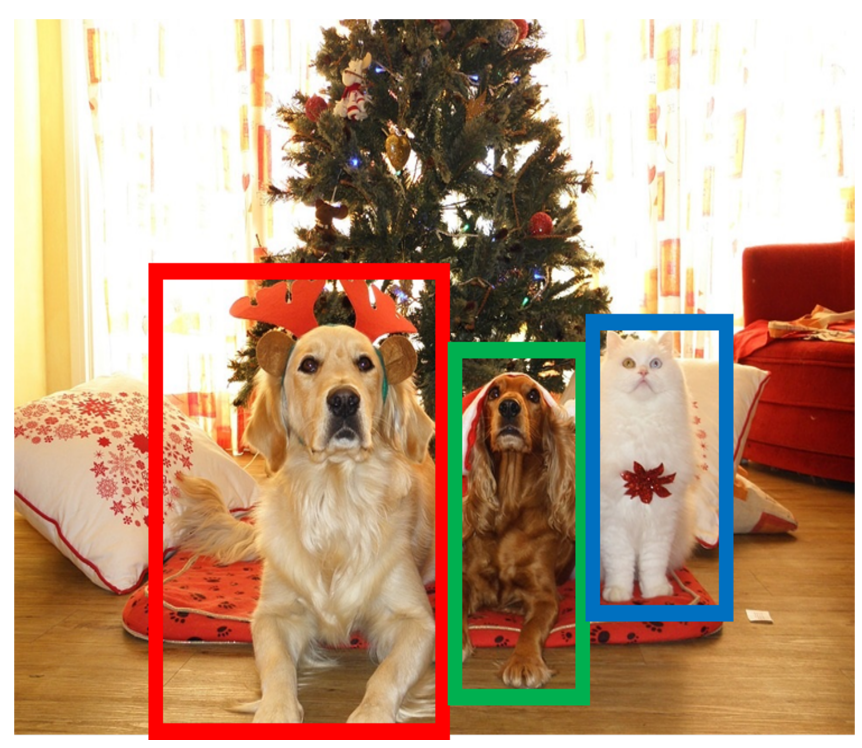
\includegraphics[width=1.0\textwidth,height=0.95\textheight,keepaspectratio]{./images/object_1.png}
\end{figure}
    
\end{frame}

\begin{frame}{Object Detection: Challenges}
\begin{itemize}
    \item \textbf{Multiple outputs:} Need to output variable numbers of objects per image
    \item \textbf{Multiple types of output:} Need to predict "what" (category label) as well as "where" (bounding box)
    \item \textbf{Large images:} Classification works at 224x224; need higher resolution for detection, often $\sim 800 \times 600$

\end{itemize}
    
\end{frame}

\begin{frame}{Comparing Boxes: Intersection over Union (IoU)}
\begin{columns}
\begin{column}{0.5\textwidth}
    \begin{itemize}
        \item How can we compare our prediction to the ground-truth box?
        
        \item<2-> \textbf{Intersection over Union} (IoU) (Also called "Jaccard similarity" or "Jaccard index"):
        $$\frac{\text{Area of Intersection}}{\text{Area of Union}}$$
    \end{itemize}
\end{column}

\begin{column}{0.5\textwidth}
    \begin{figure}
    \centering
    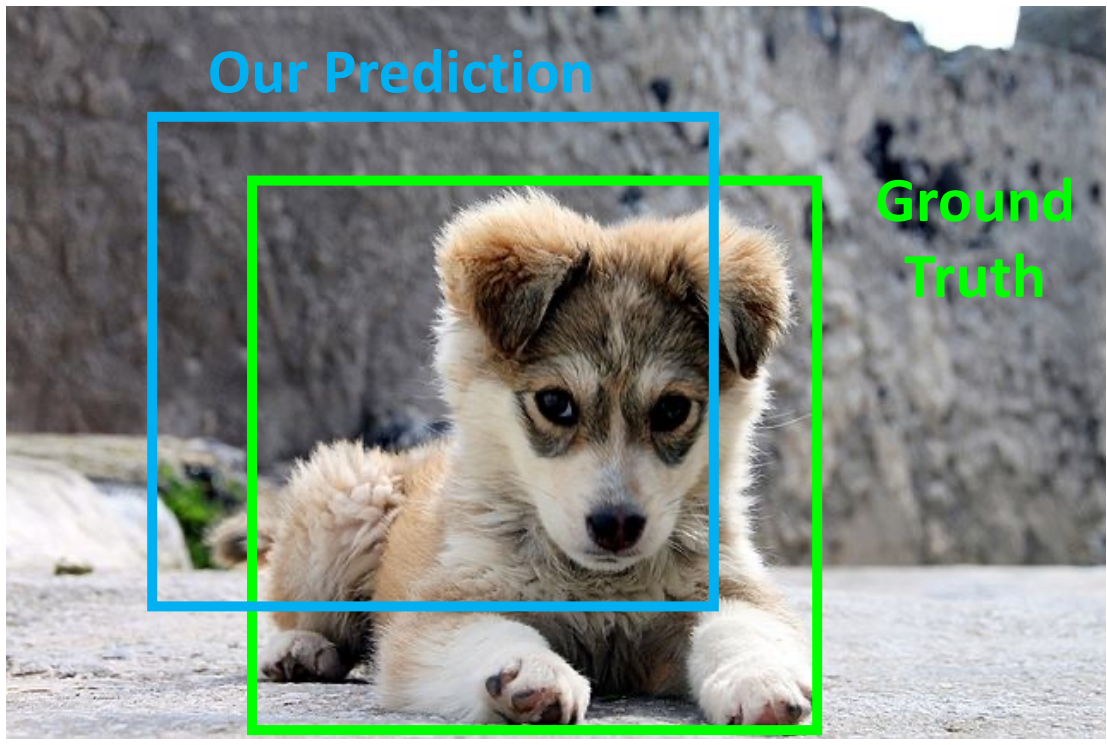
\includegraphics[width=1.0\textwidth,height=1.0\textheight,keepaspectratio]{./images/object_2.png}
    \end{figure}
\end{column}

\end{columns}
    
\end{frame}

\begin{frame}[allowframebreaks]{Detecting a Single Object}
\begin{figure}
\centering
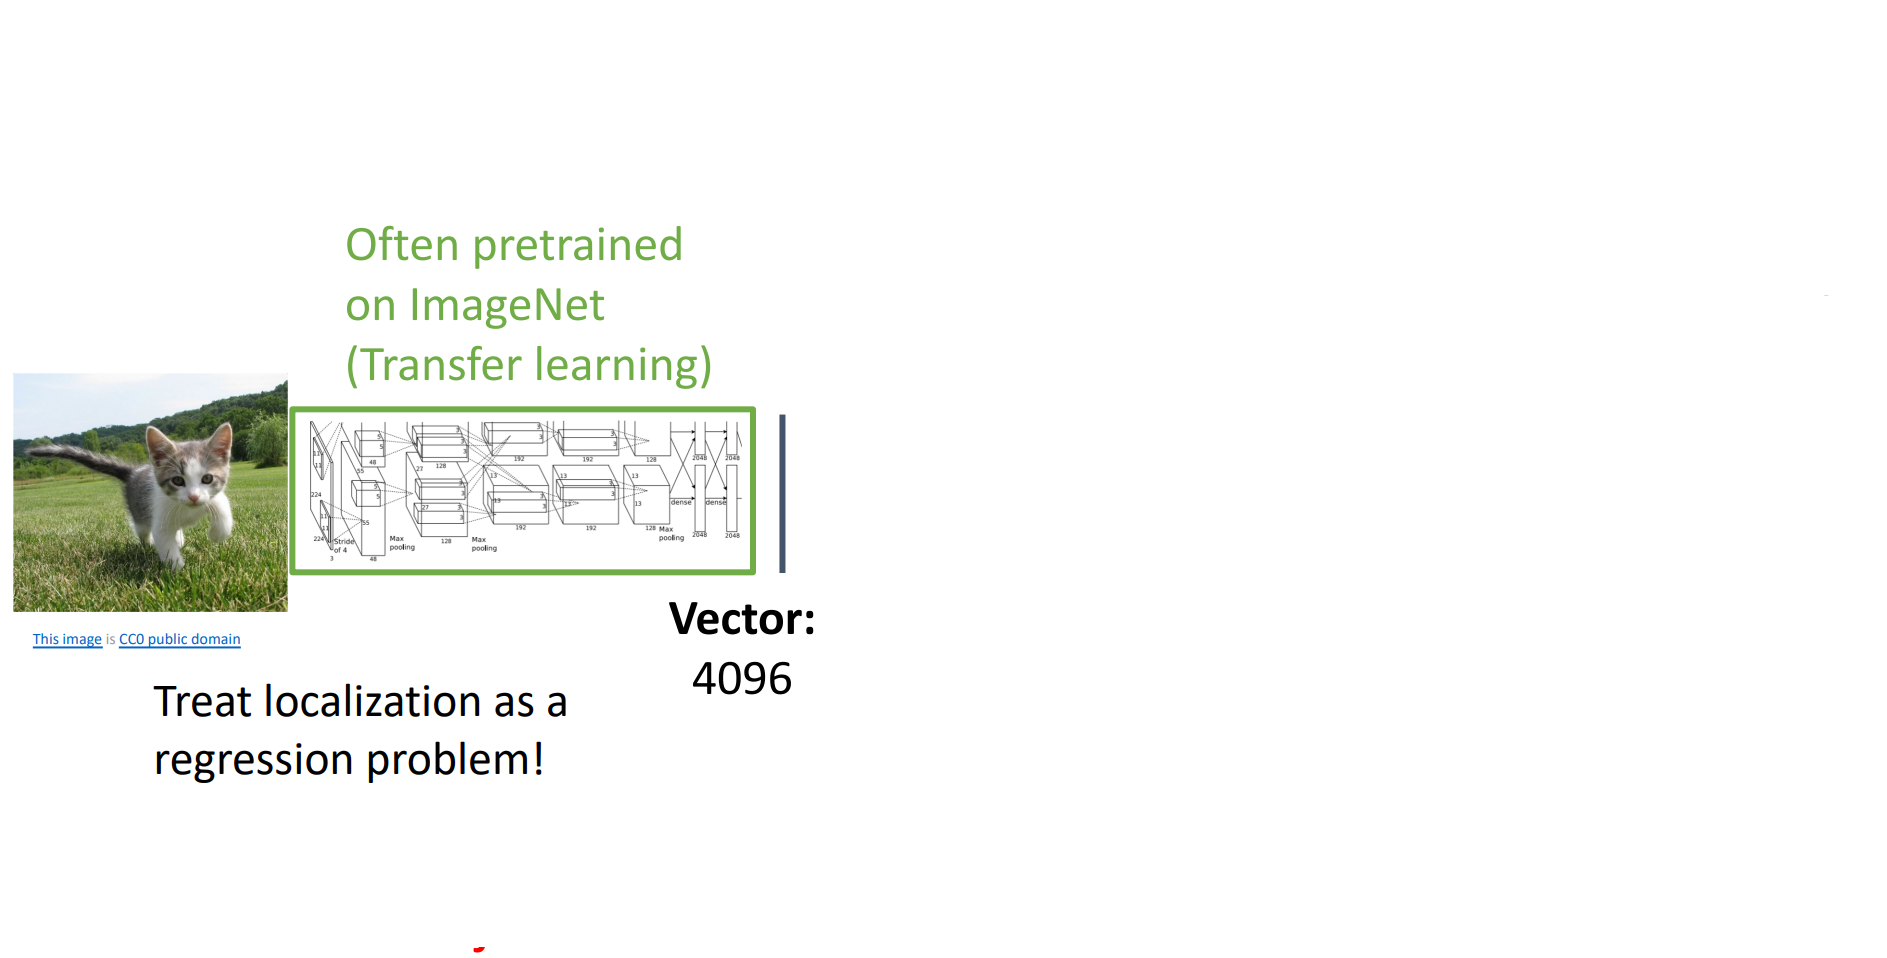
\includegraphics[width=1.0\textwidth,height=1.0\textheight,keepaspectratio]{./images/object_3.png}
\end{figure}

\framebreak

\begin{figure}
\centering
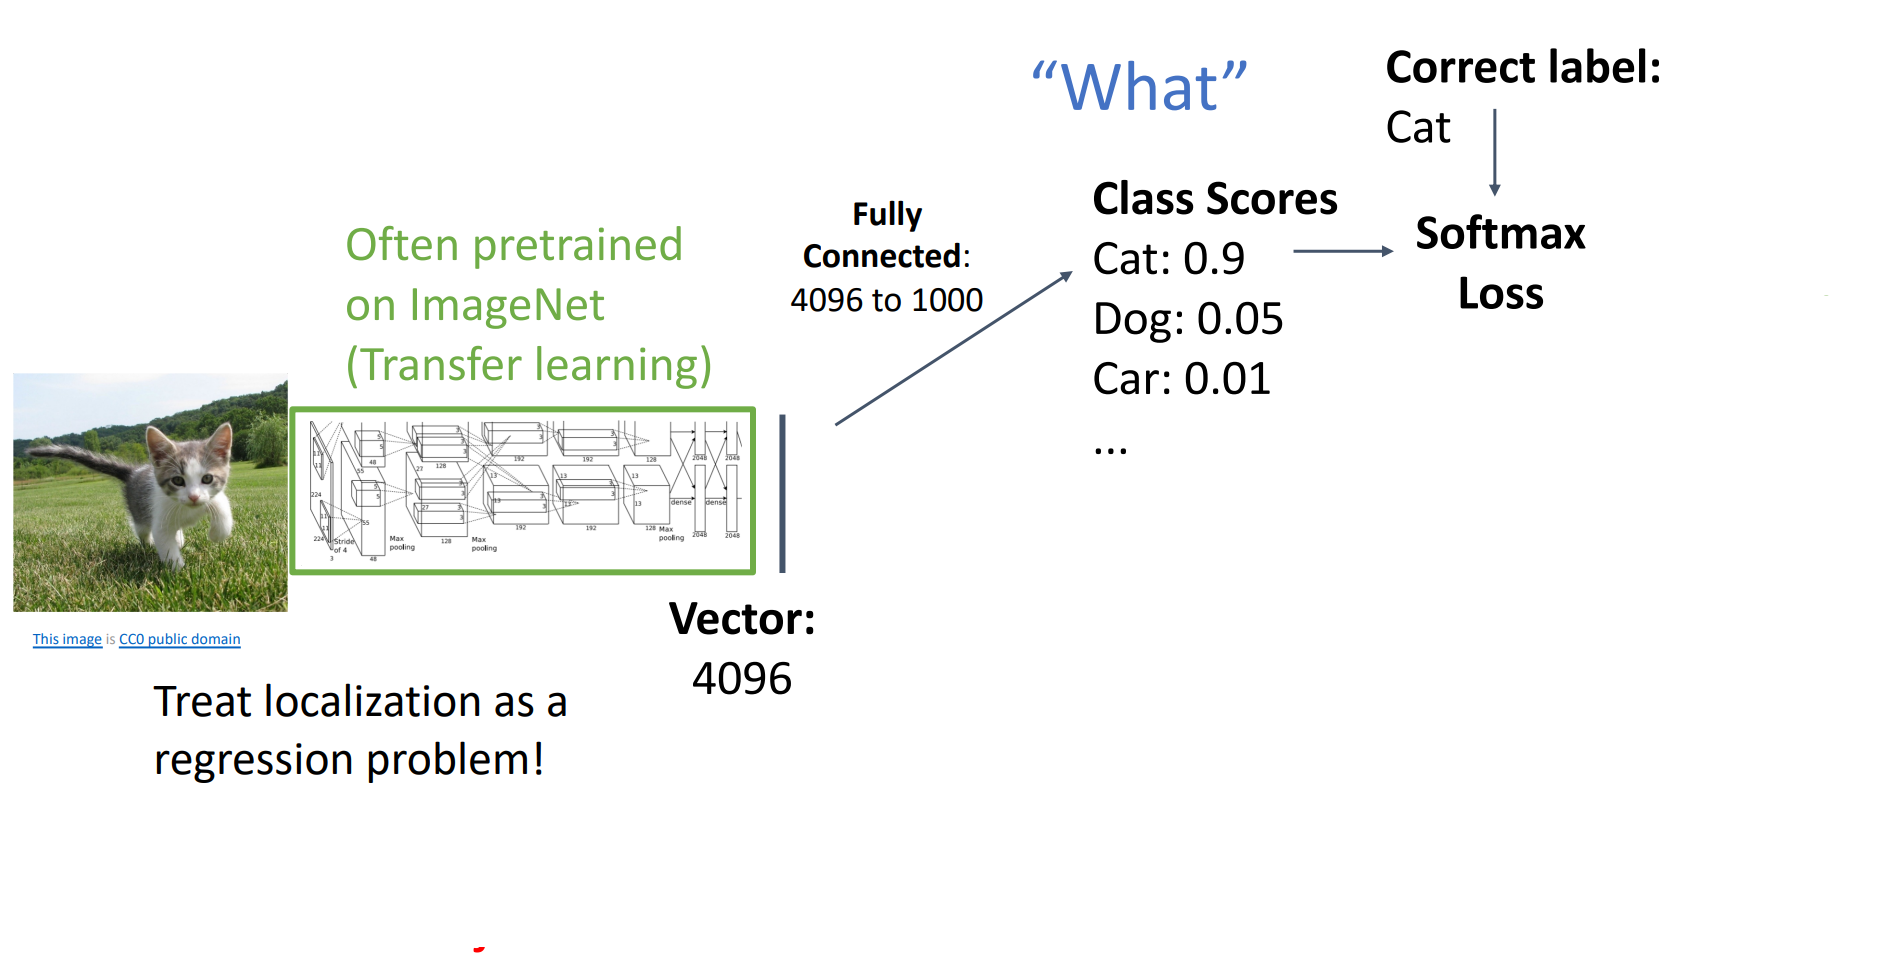
\includegraphics[width=1.0\textwidth,height=1.0\textheight,keepaspectratio]{./images/object_4.png}
\end{figure}

\framebreak

\begin{figure}
\centering
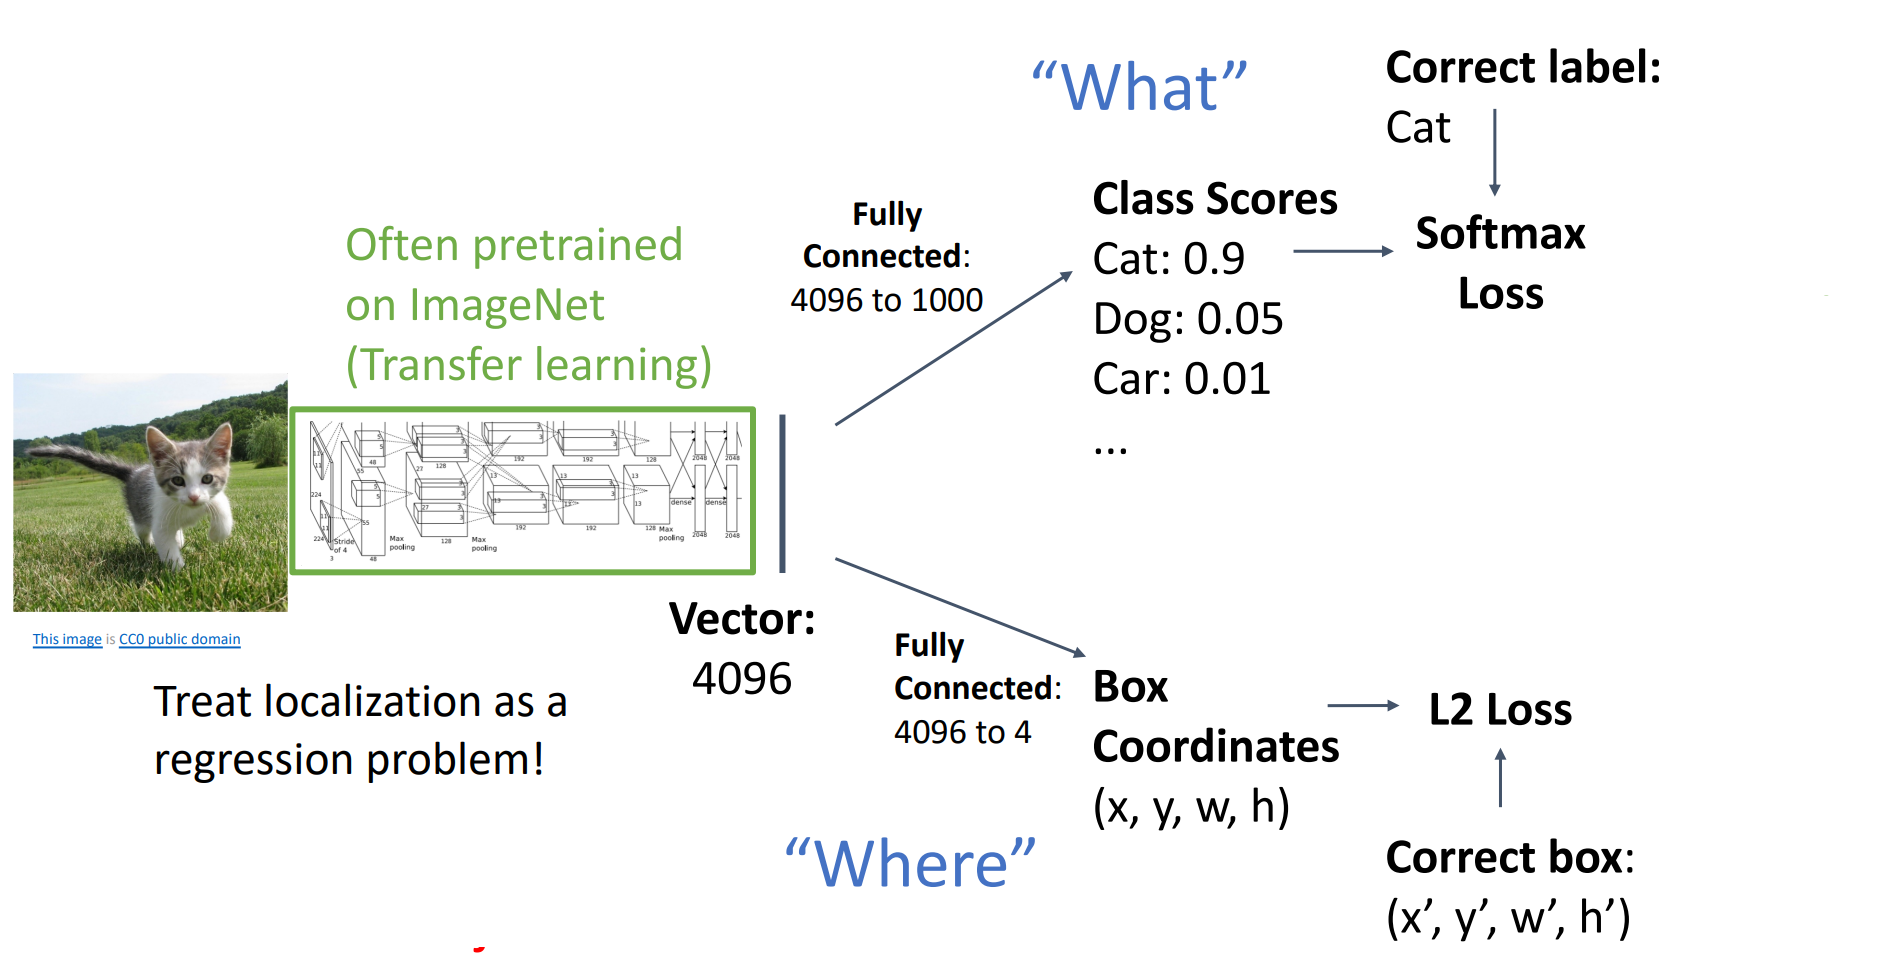
\includegraphics[width=1.0\textwidth,height=1.0\textheight,keepaspectratio]{./images/object_5.png}
\end{figure}

\framebreak

\begin{figure}
\centering
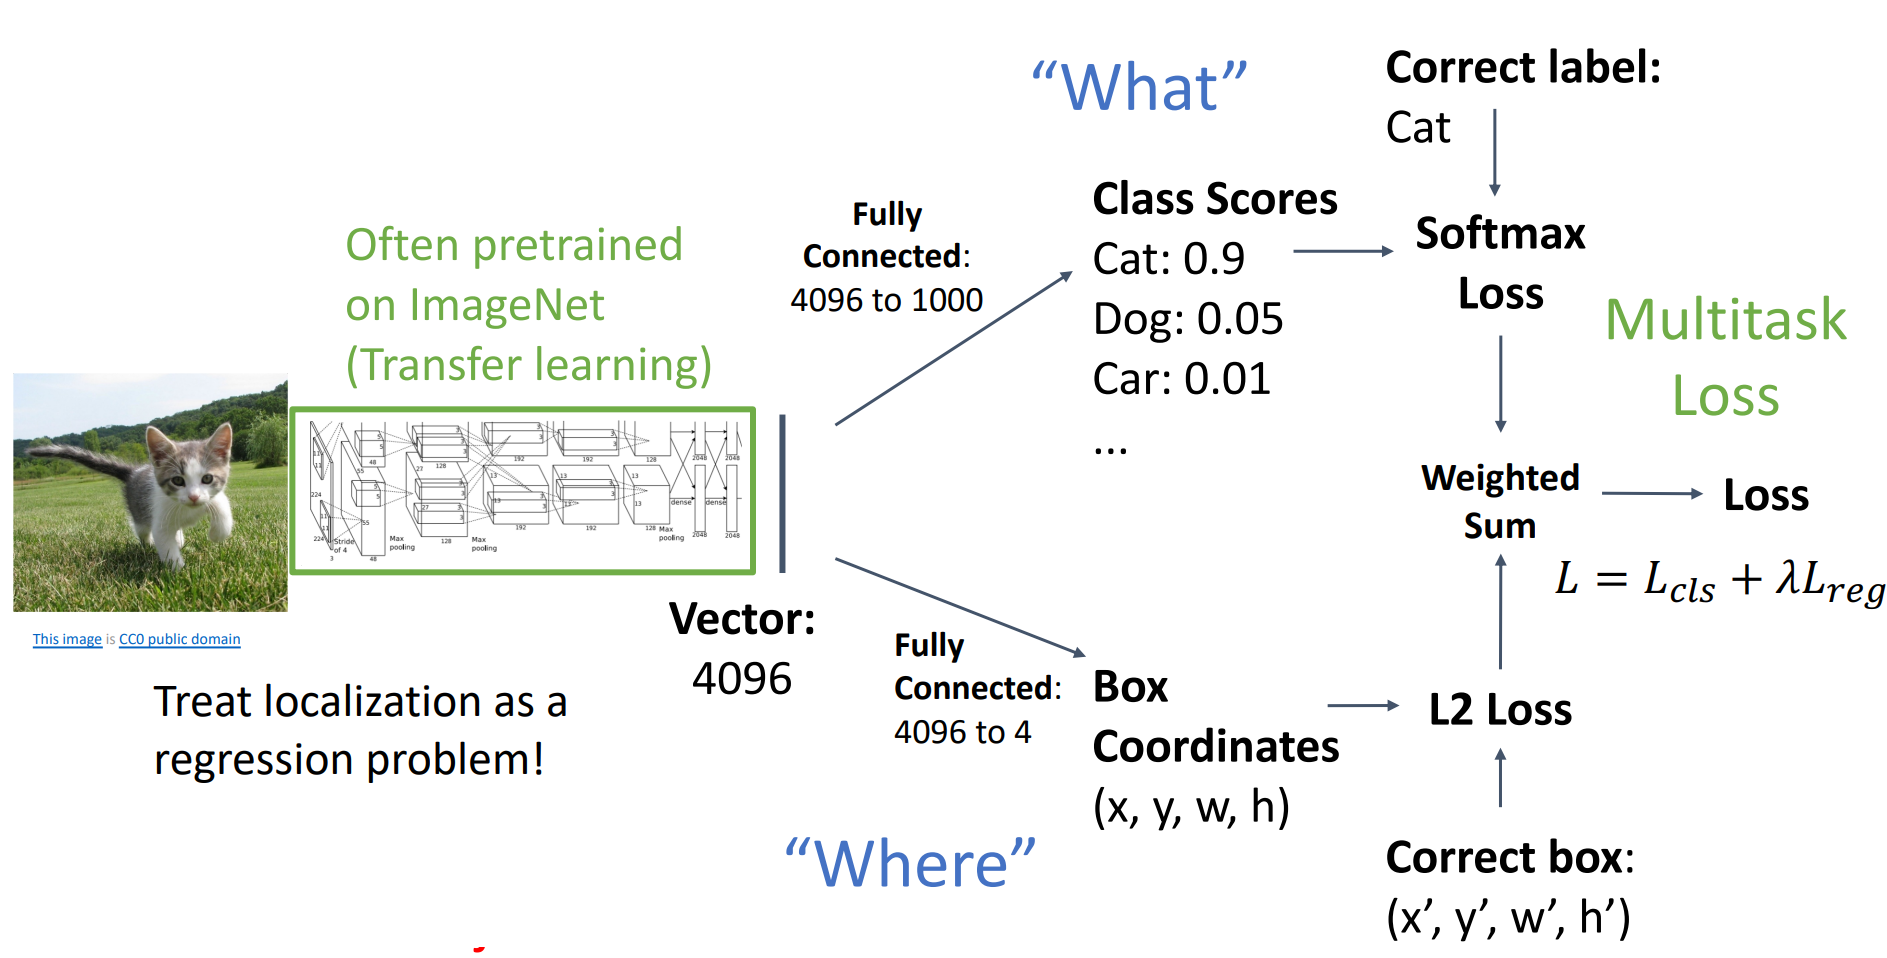
\includegraphics[width=1.0\textwidth,height=1.0\textheight,keepaspectratio]{./images/object_6.png}
\end{figure}

\framebreak

\begin{figure}
\centering
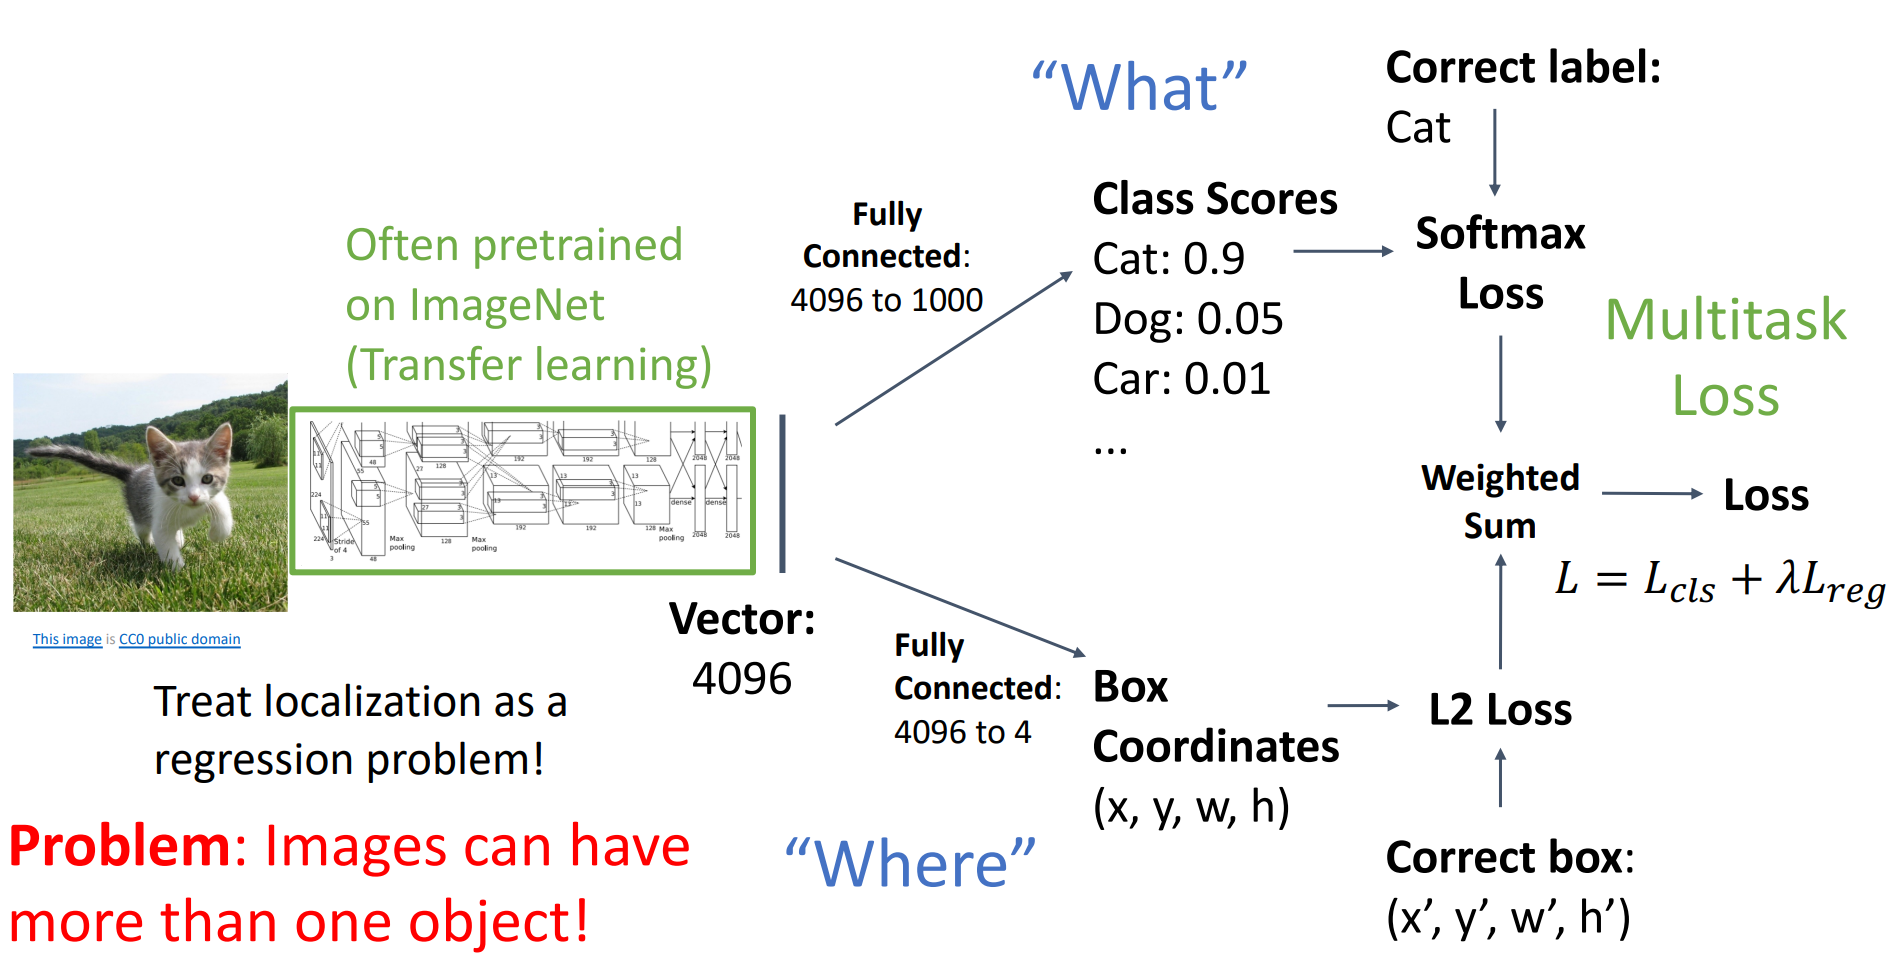
\includegraphics[width=1.0\textwidth,height=1.0\textheight,keepaspectratio]{./images/object_7.png}
\end{figure}
    
\end{frame}

\begin{frame}[allowframebreaks]{Multiple Objects}

\begin{figure}
\centering
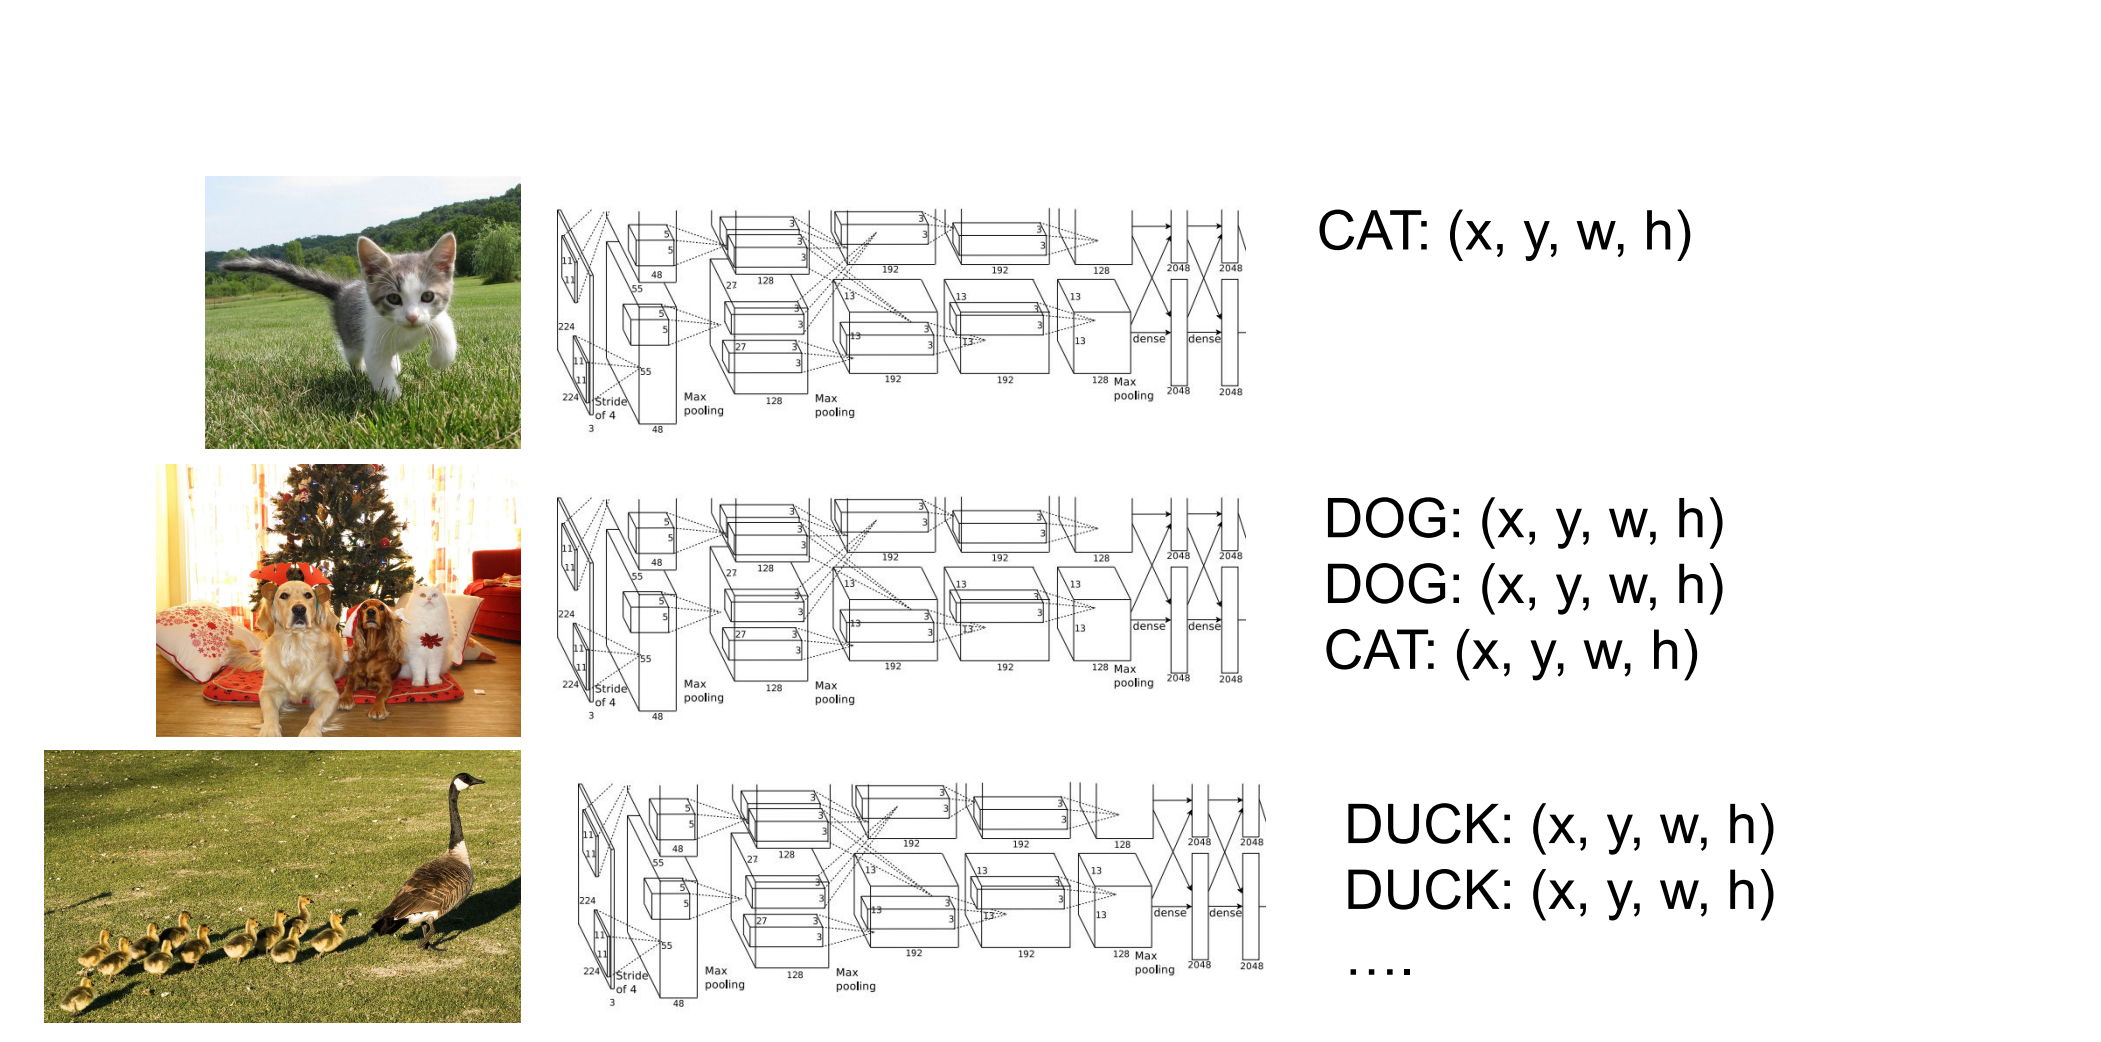
\includegraphics[width=1.0\textwidth,height=1.0\textheight,keepaspectratio]{./images/object_8.png}
\end{figure}

\framebreak

\begin{figure}
\centering
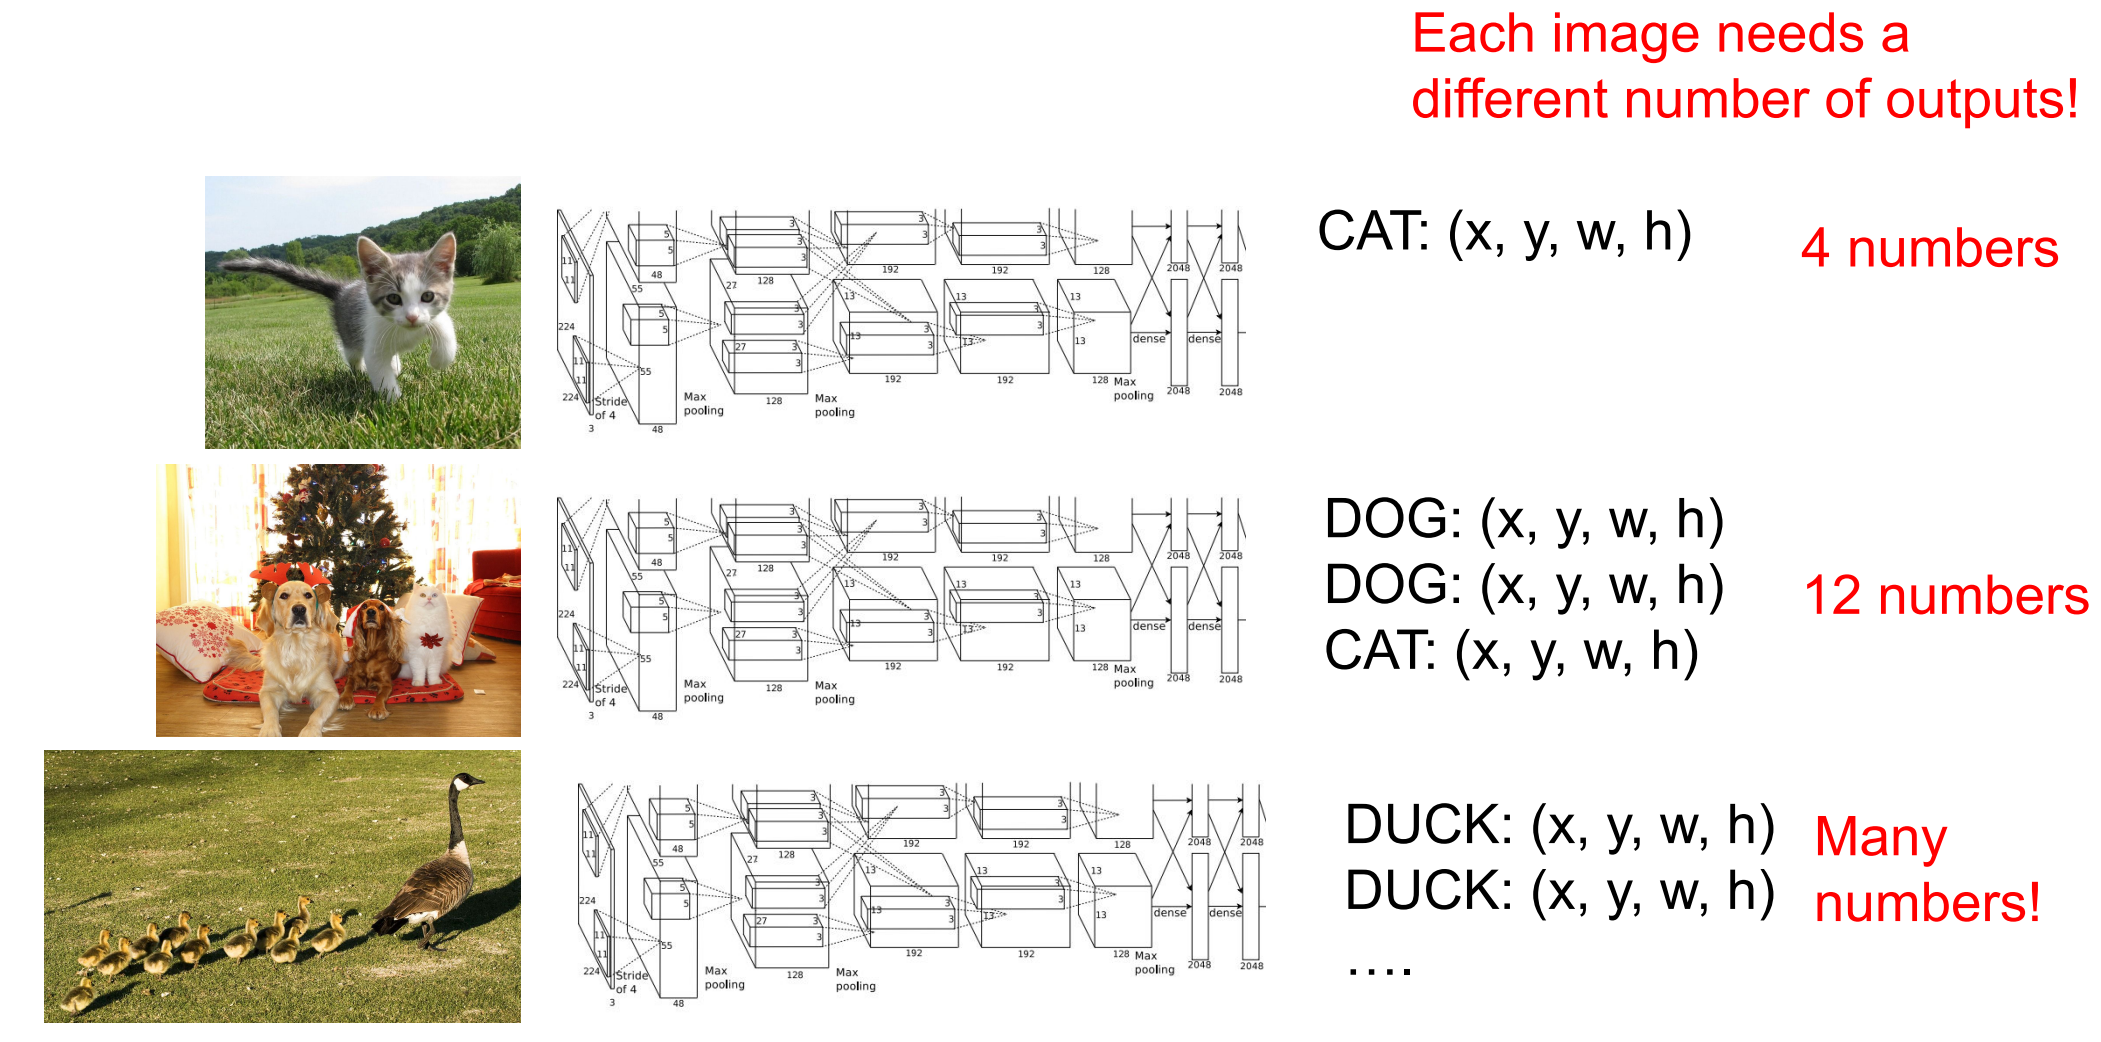
\includegraphics[width=1.0\textwidth,height=1.0\textheight,keepaspectratio]{./images/object_9.png}
\end{figure}

\end{frame}

\begin{frame}[allowframebreaks]{Detecting Multiple Objects: Sliding Window}

\begin{figure}
\centering
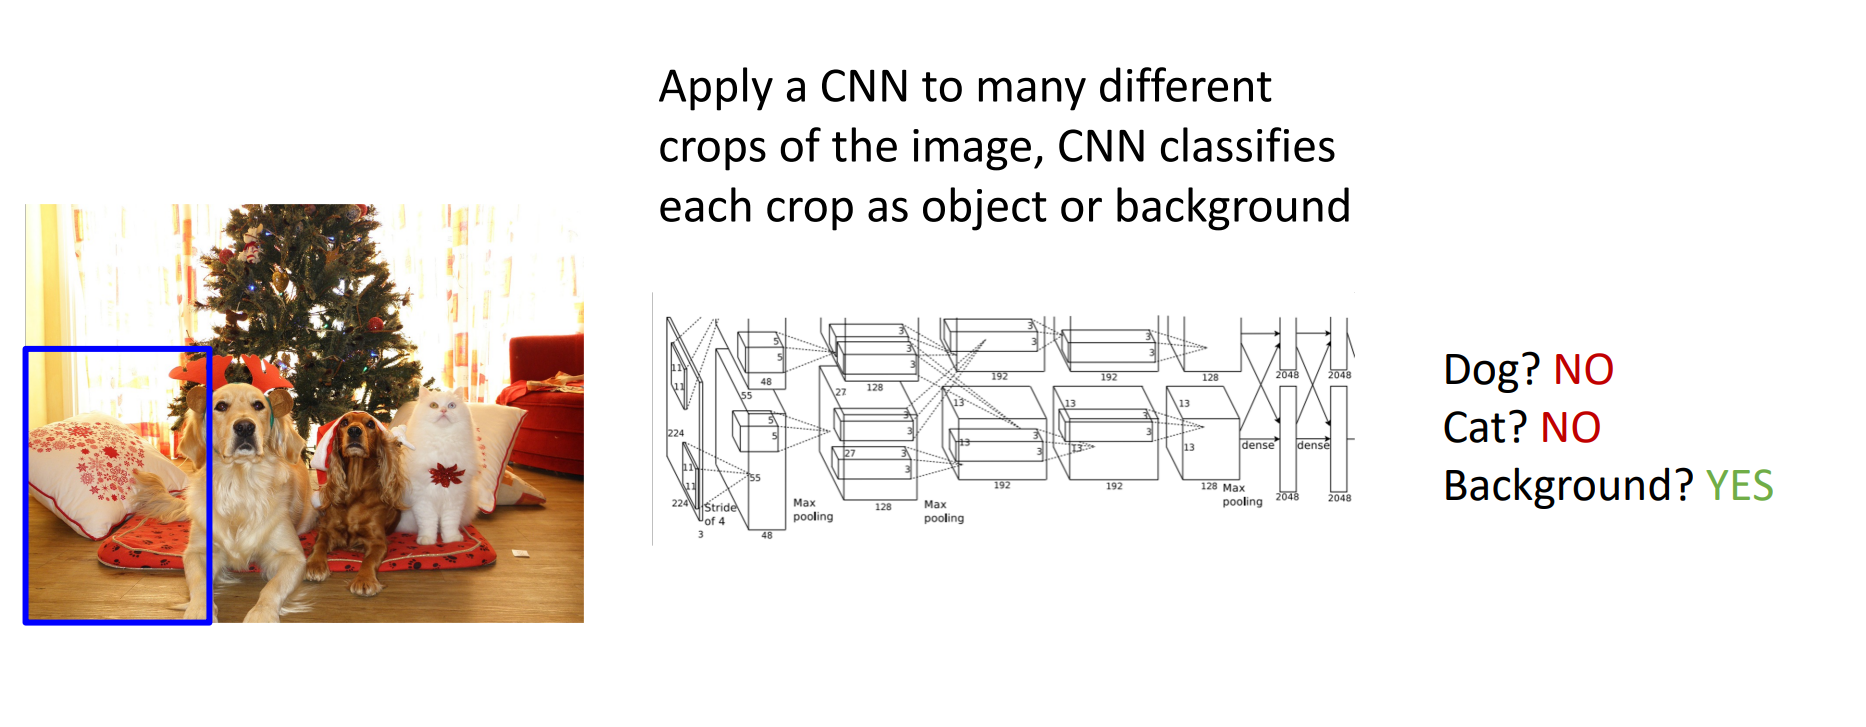
\includegraphics[width=1.0\textwidth,height=1.0\textheight,keepaspectratio]{./images/object_10.png}
\end{figure}

\framebreak

\begin{figure}
\centering
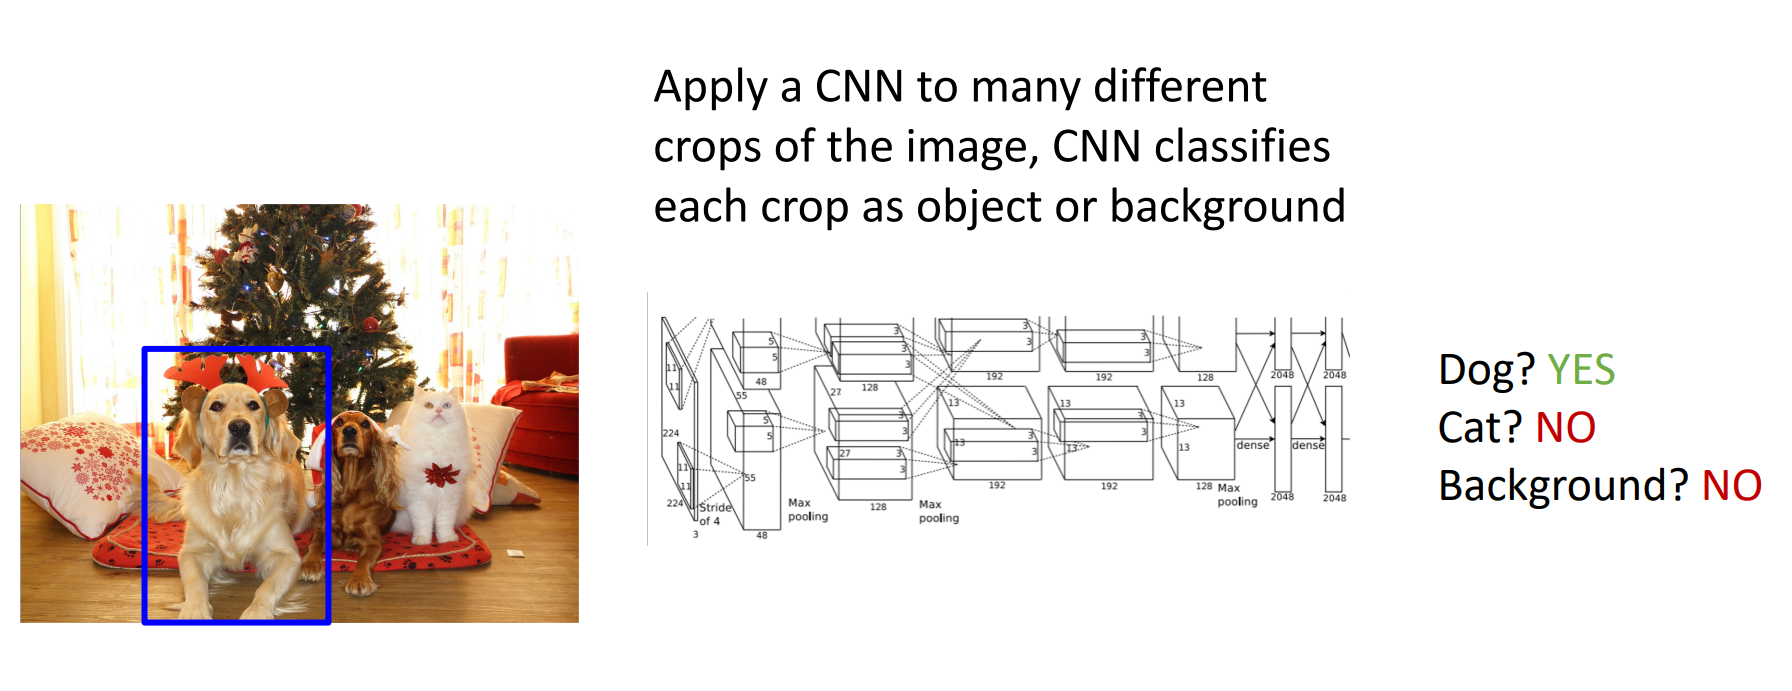
\includegraphics[width=1.0\textwidth,height=1.0\textheight,keepaspectratio]{./images/object_11.png}
\end{figure}

\framebreak

\begin{figure}
\centering
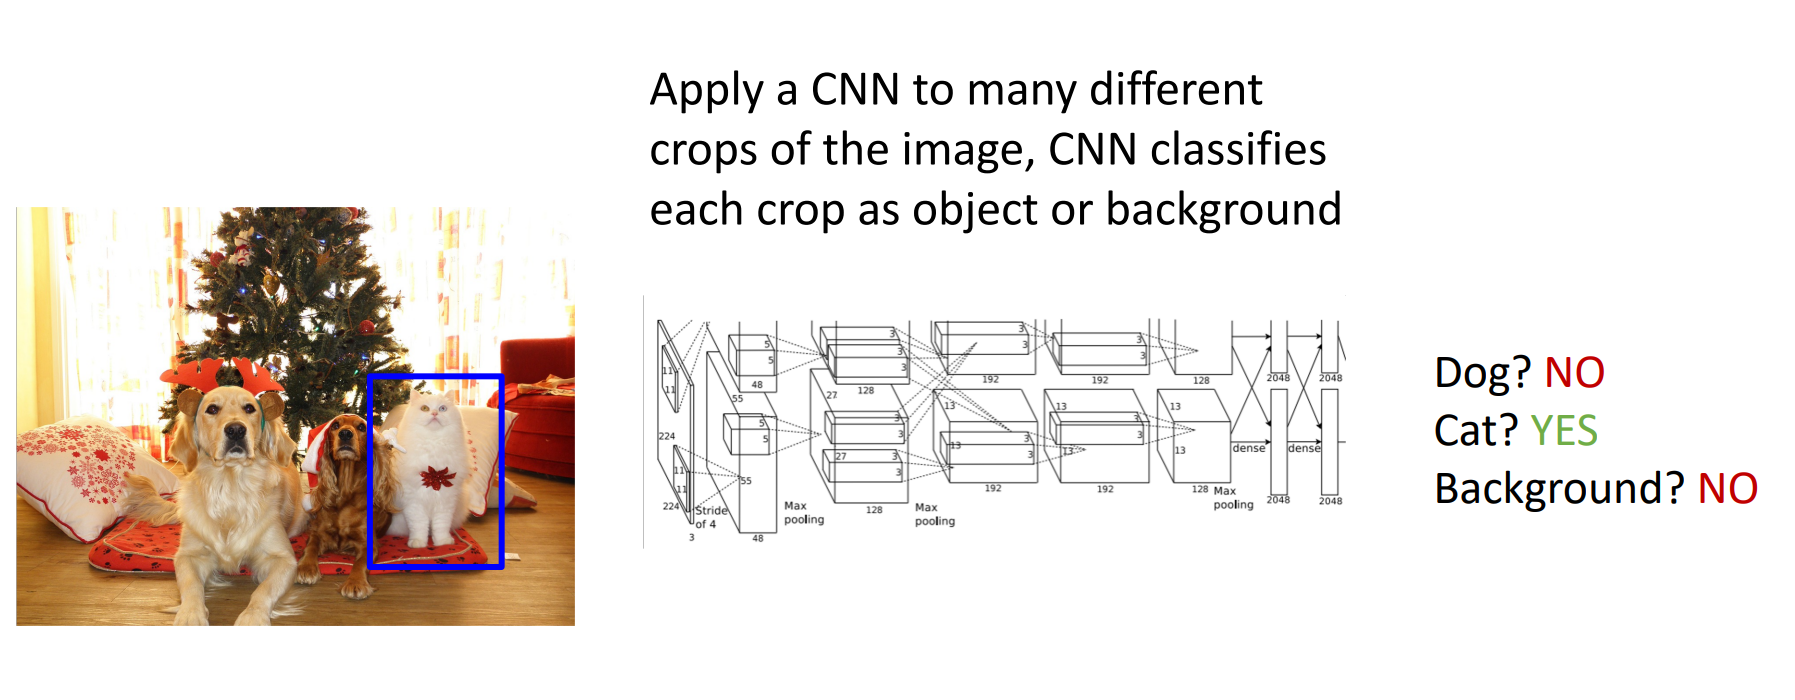
\includegraphics[width=1.0\textwidth,height=1.0\textheight,keepaspectratio]{./images/object_12.png}
\end{figure}

\framebreak

\begin{figure}
\centering
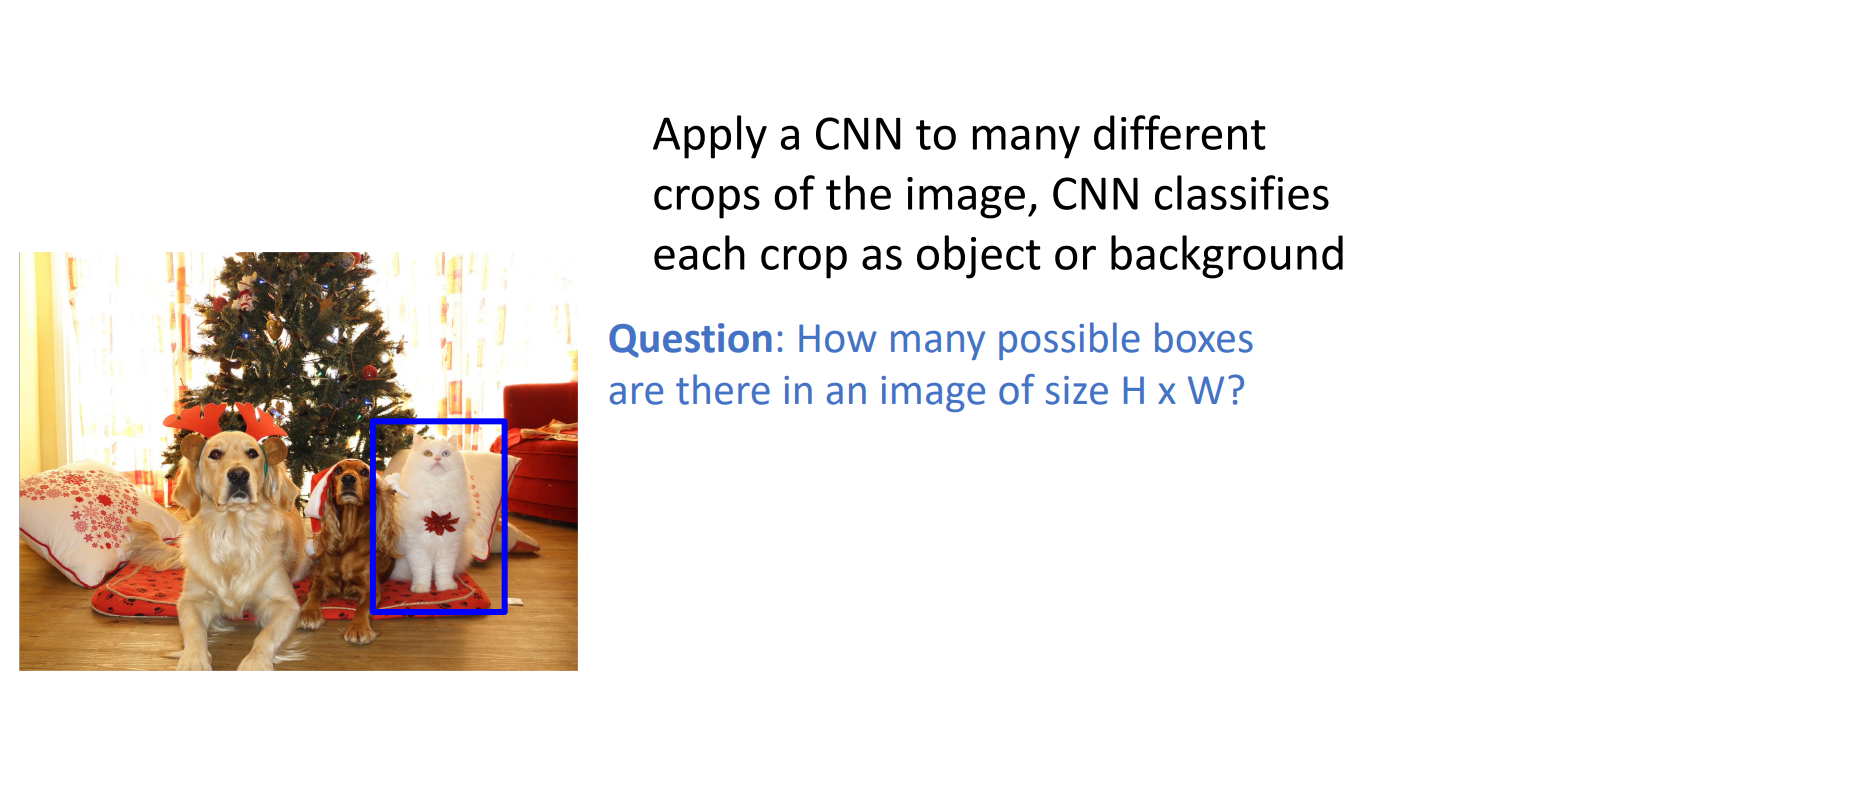
\includegraphics[width=1.0\textwidth,height=1.0\textheight,keepaspectratio]{./images/object_13.png}
\end{figure}

\framebreak

\begin{figure}
\centering
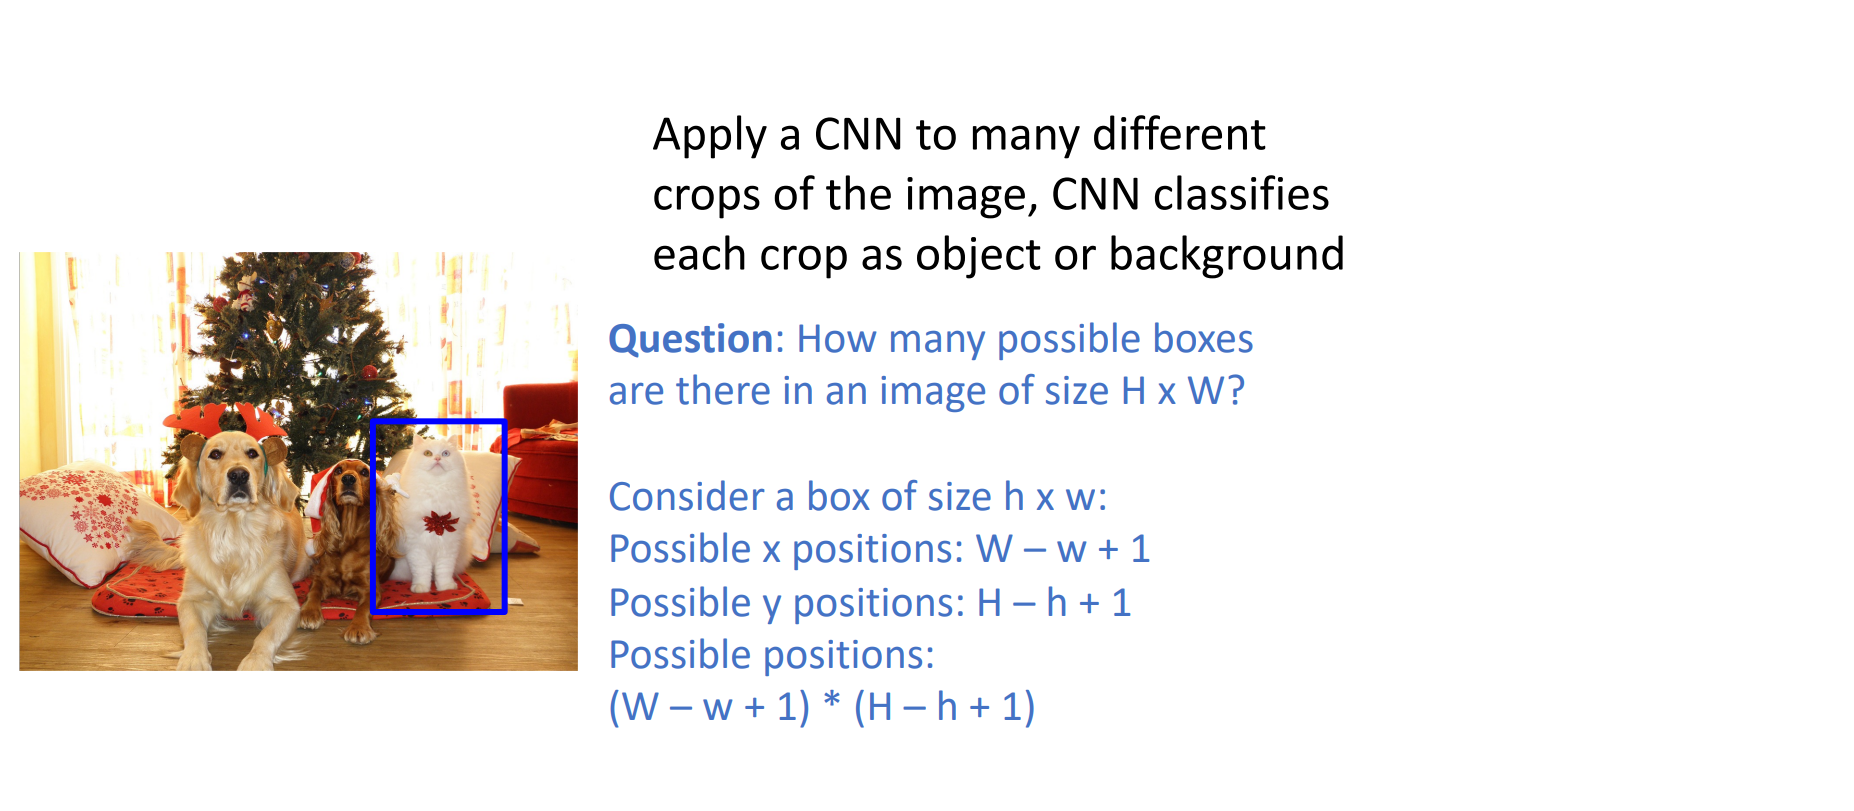
\includegraphics[width=1.0\textwidth,height=1.0\textheight,keepaspectratio]{./images/object_14.png}
\end{figure}

\framebreak

\begin{figure}
\centering
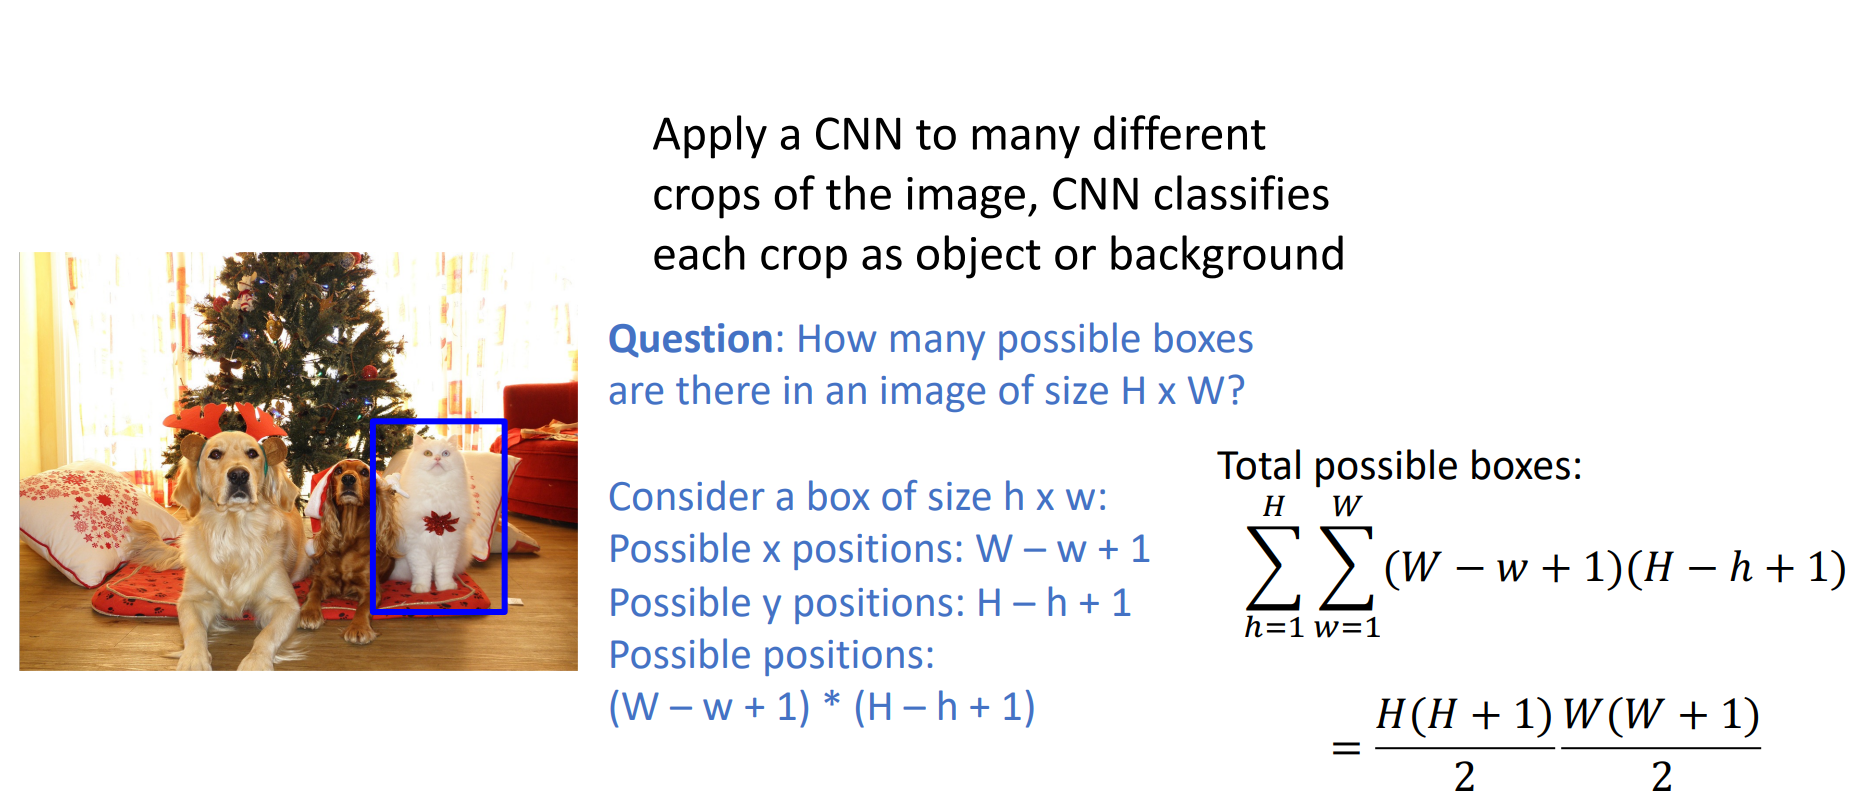
\includegraphics[width=1.0\textwidth,height=1.0\textheight,keepaspectratio]{./images/object_15.png}
\end{figure}

\framebreak

\begin{figure}
\centering
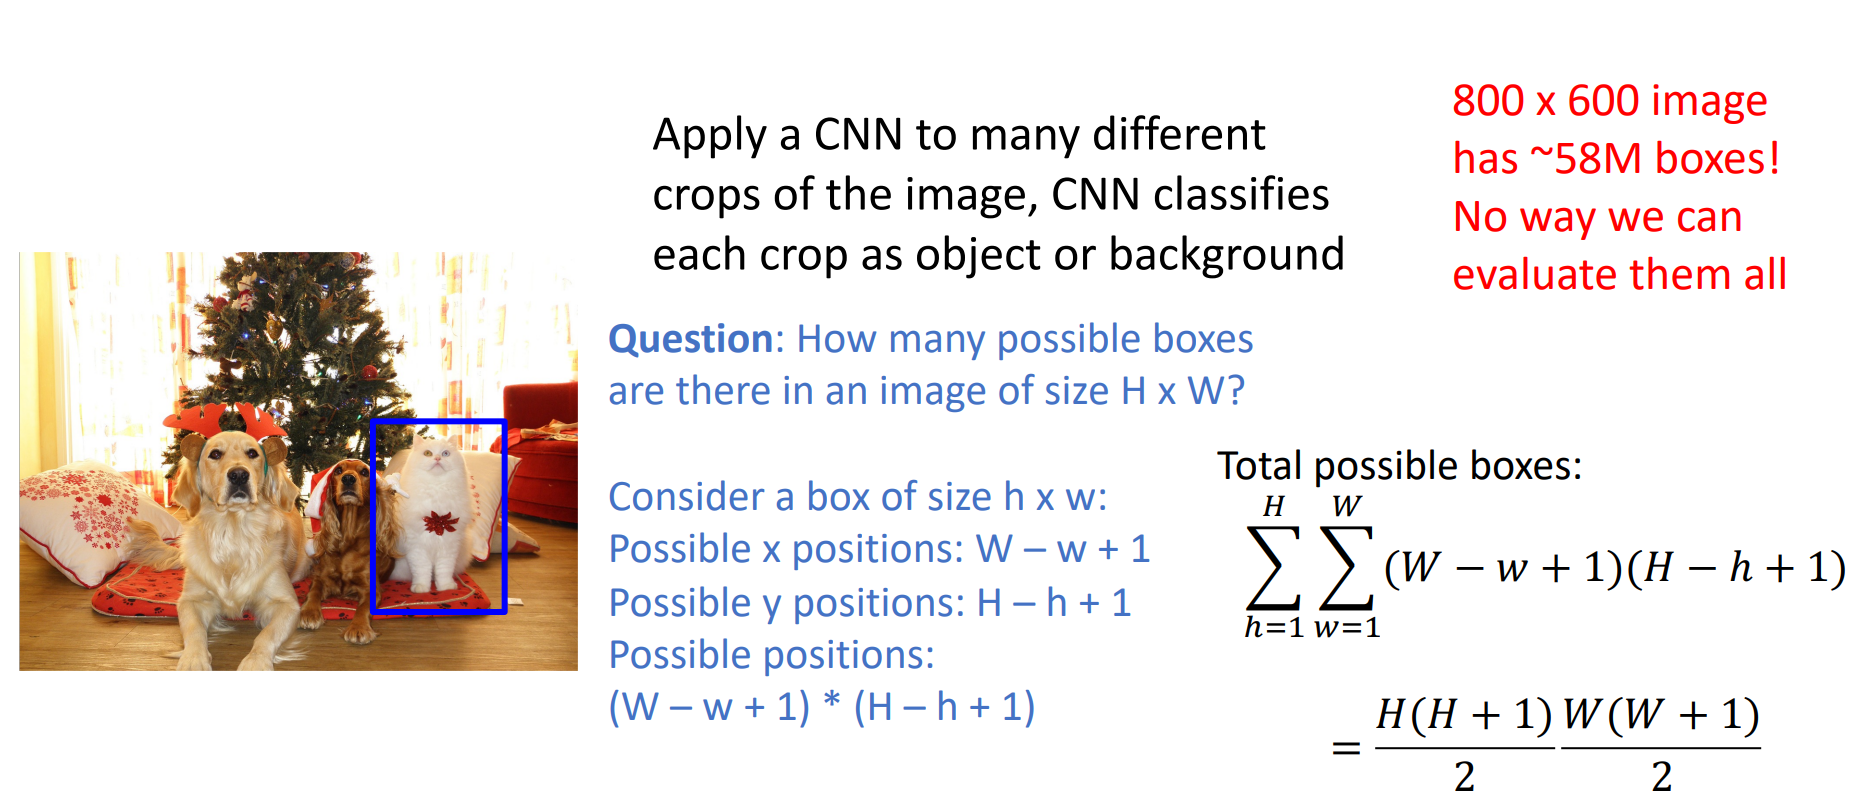
\includegraphics[width=1.0\textwidth,height=1.0\textheight,keepaspectratio]{./images/object_16.png}
\end{figure}

\end{frame}

\begin{frame}{Region Proposal}
\begin{itemize}
    \item Find a small set of boxes that are likely to cover all objects
    \item Often based on heuristics: e.g. look for “blob-like” image regions
    \item Relatively fast to run; e.g. Selective Search gives 2000 region proposals in a few seconds on CPU

\end{itemize}
\begin{figure}
\centering
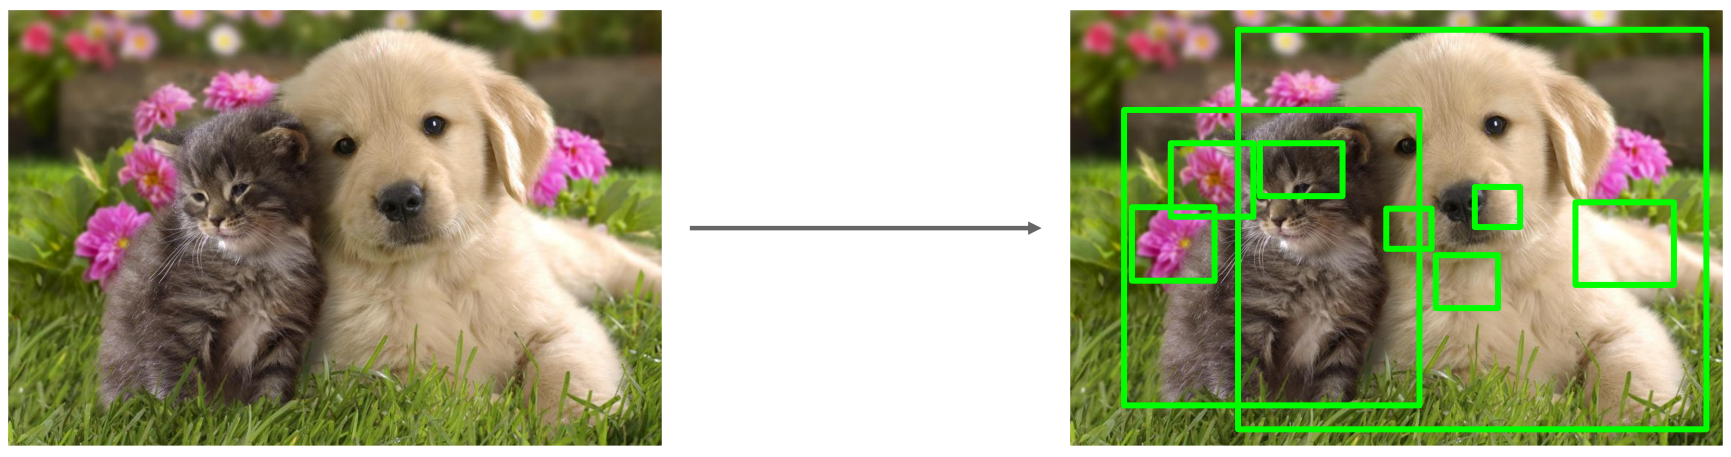
\includegraphics[width=1.0\textwidth,height=1.0\textheight,keepaspectratio]{./images/object_17.png}
\end{figure}
    
\end{frame}

\begin{frame}[allowframebreaks]{R-CNN}

\begin{figure}
\centering
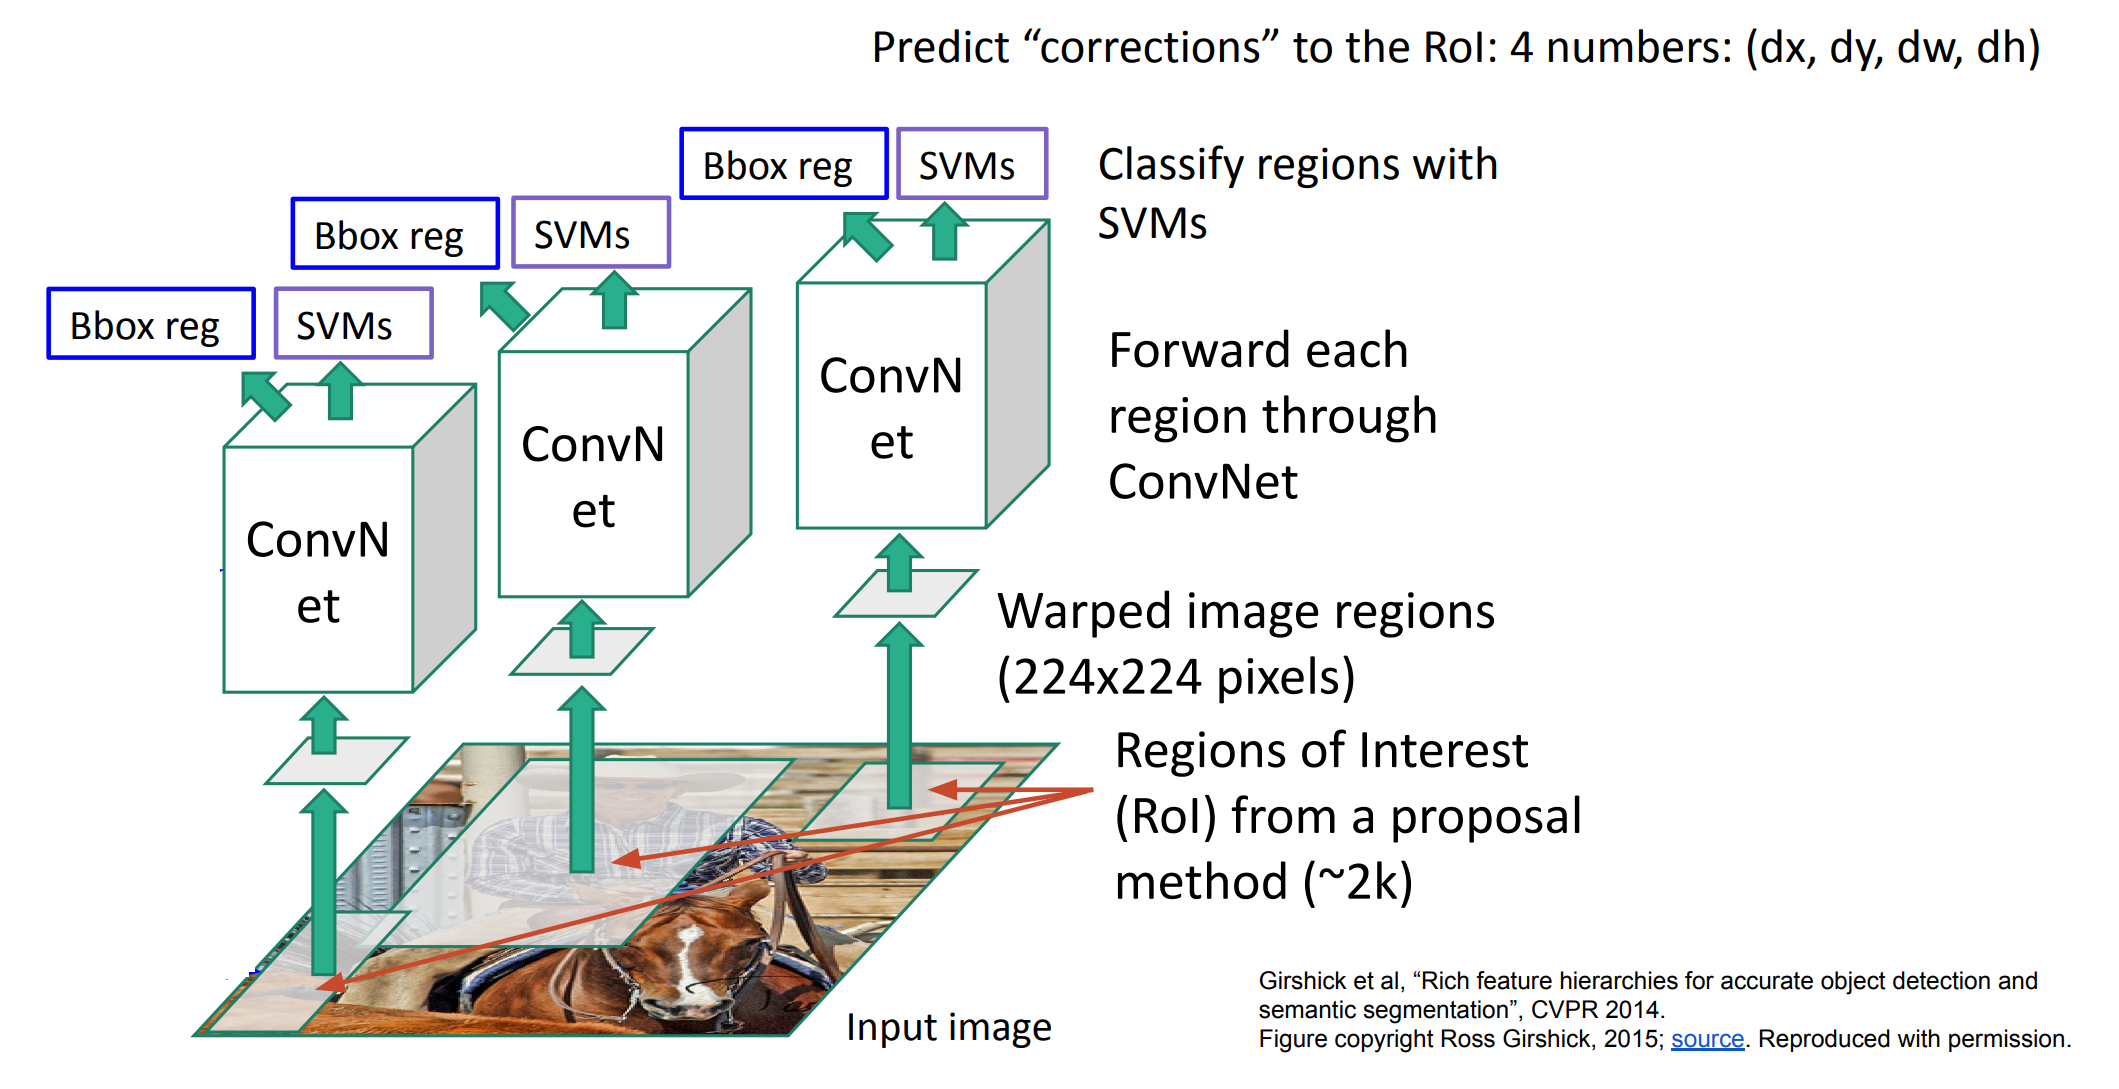
\includegraphics[width=1.0\textwidth,height=1.0\textheight,keepaspectratio]{./images/rcnn_1.png}
\end{figure}

\framebreak

\begin{figure}
\centering
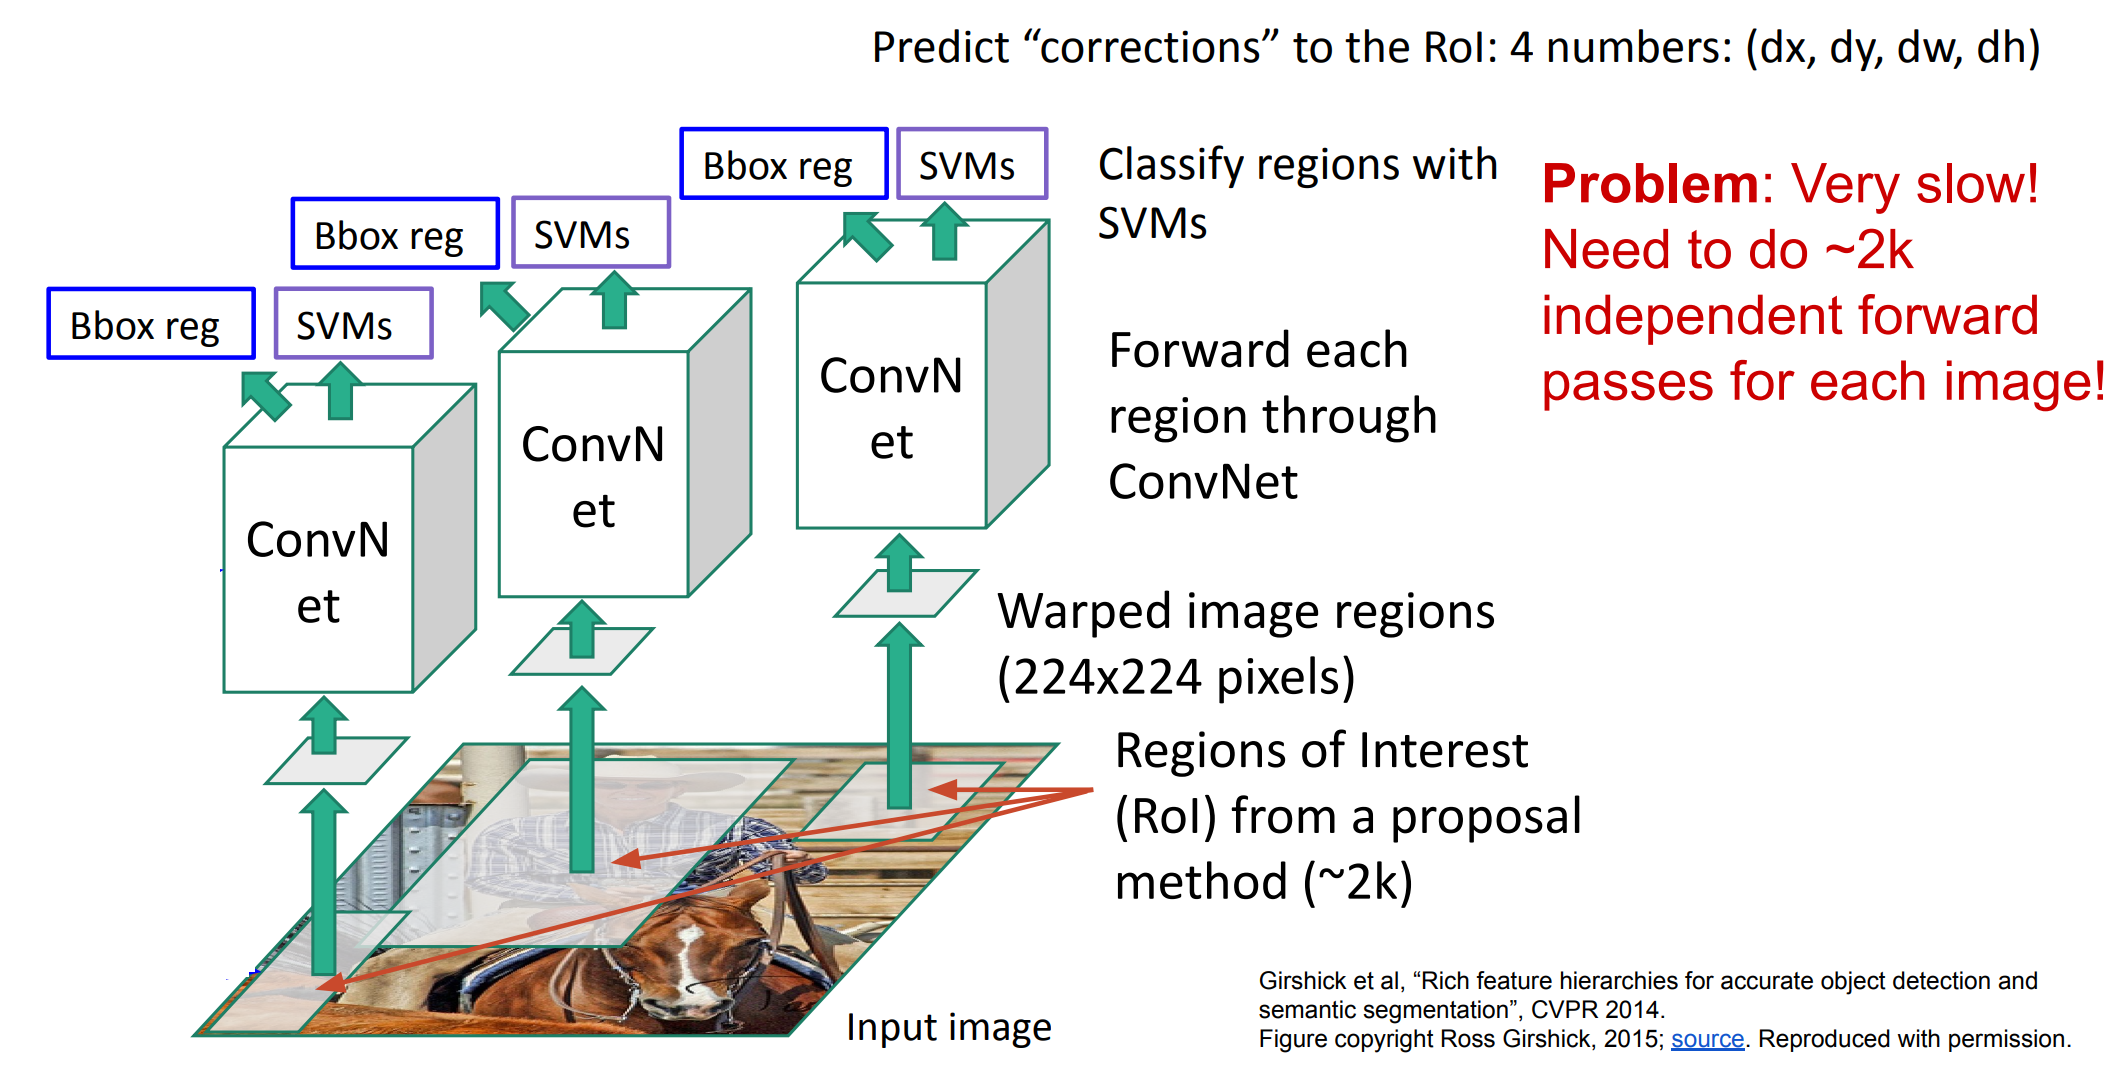
\includegraphics[width=1.0\textwidth,height=1.0\textheight,keepaspectratio]{./images/rcnn_2.png}
\end{figure}

\framebreak

\begin{figure}
\centering
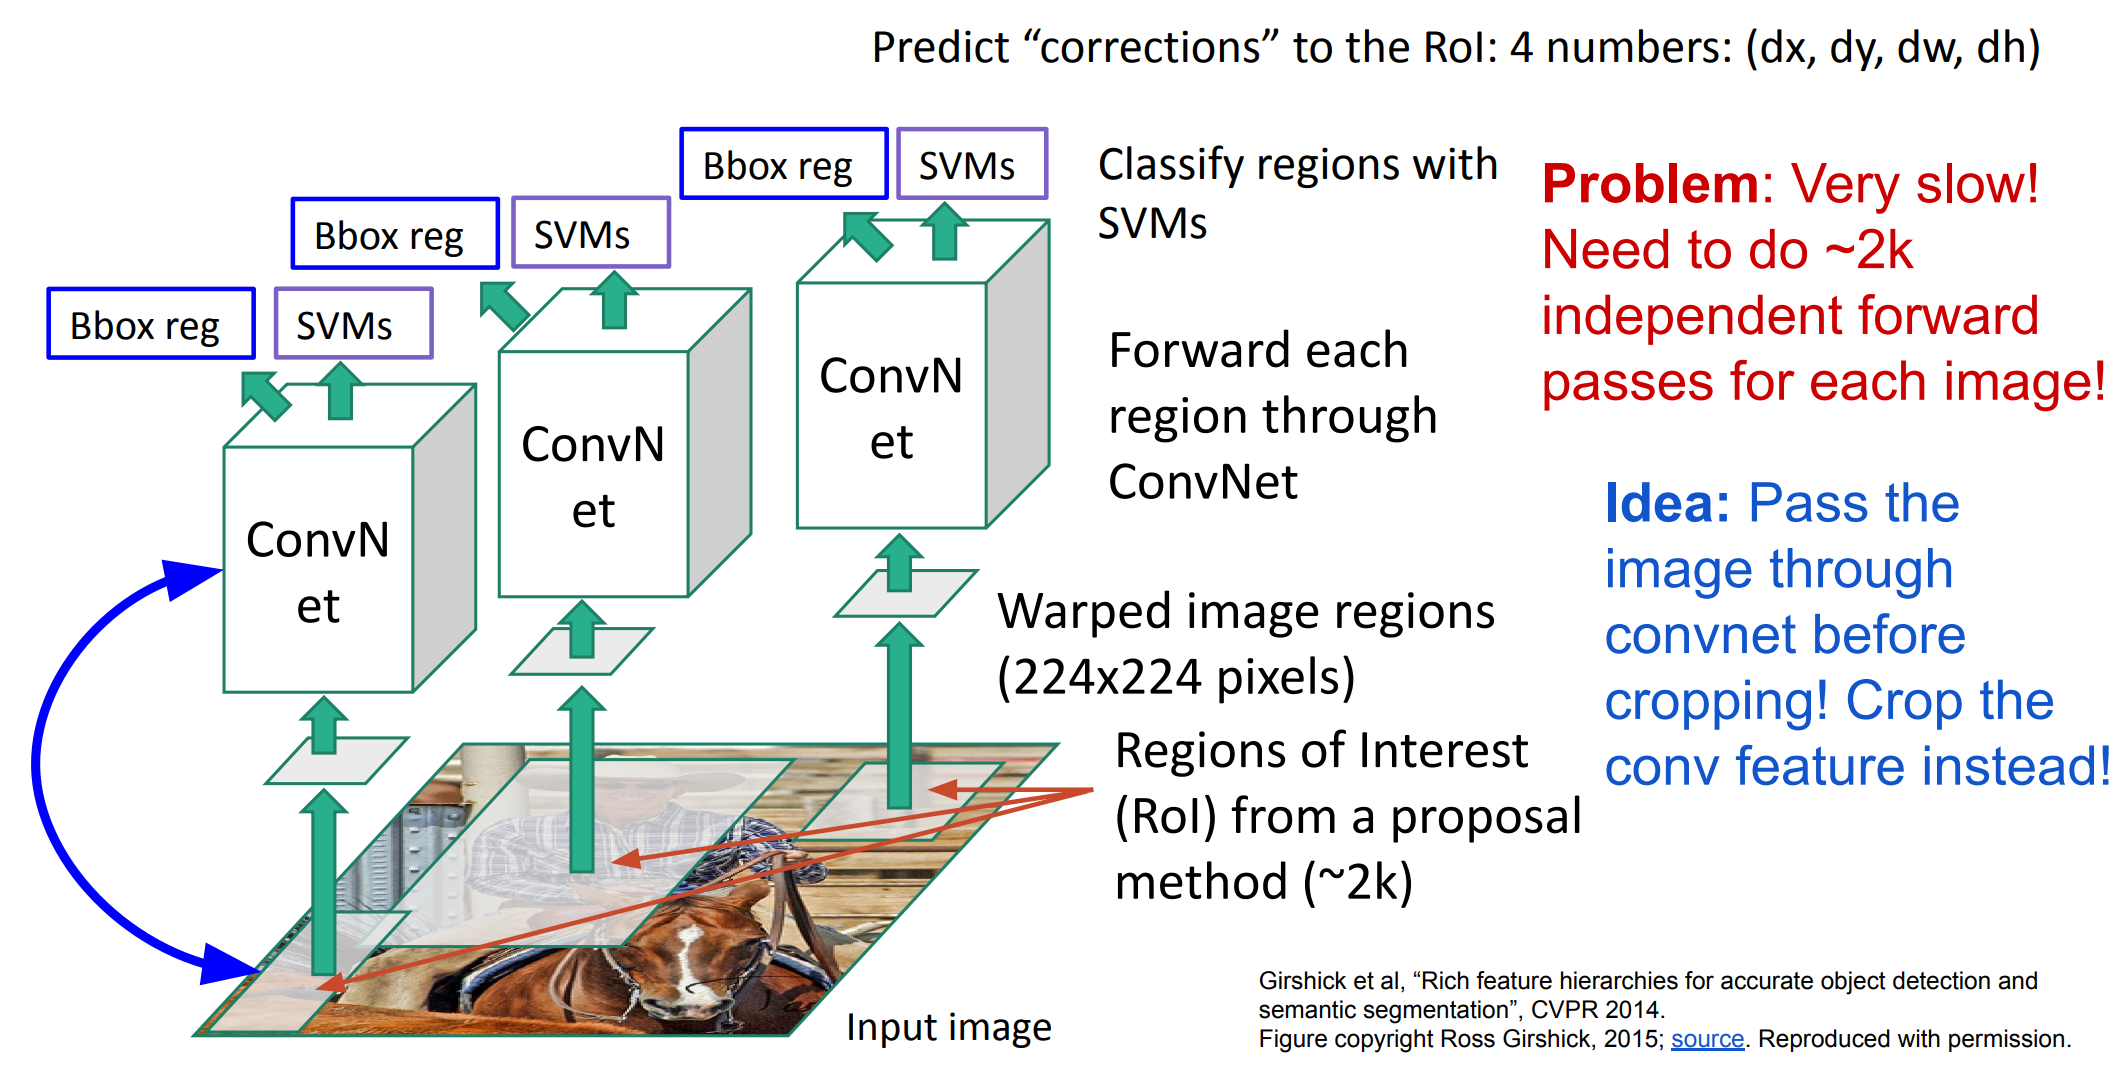
\includegraphics[width=1.0\textwidth,height=1.0\textheight,keepaspectratio]{./images/rcnn_3.png}
\end{figure}

    
\end{frame}

\begin{frame}{Fast R-CNN}
\begin{figure}
\centering
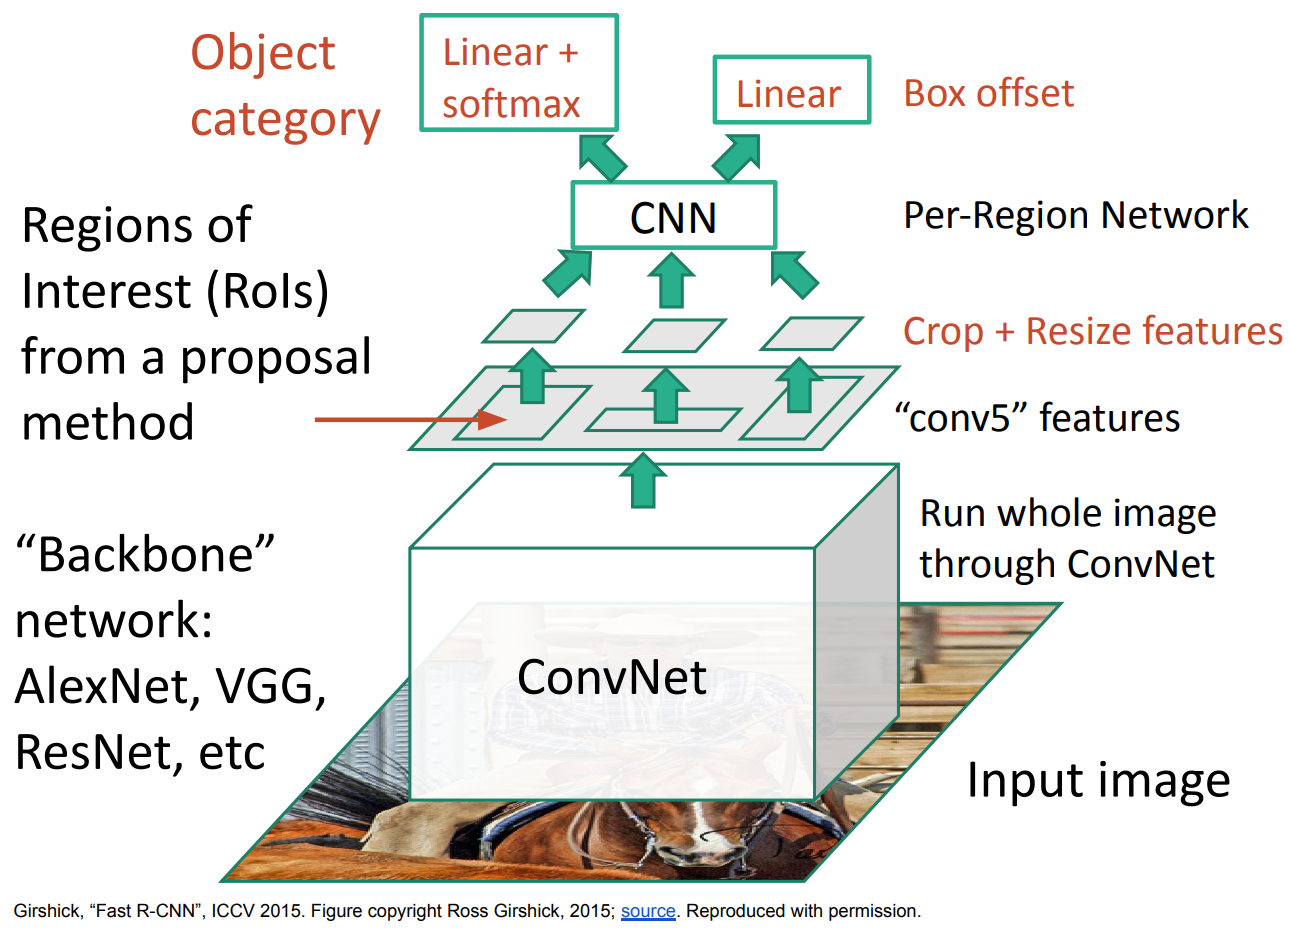
\includegraphics[width=1.0\textwidth,height=1.0\textheight,keepaspectratio]{./images/fast_rcnn_1.png}
\end{figure}

\framebreak

\begin{figure}
\centering
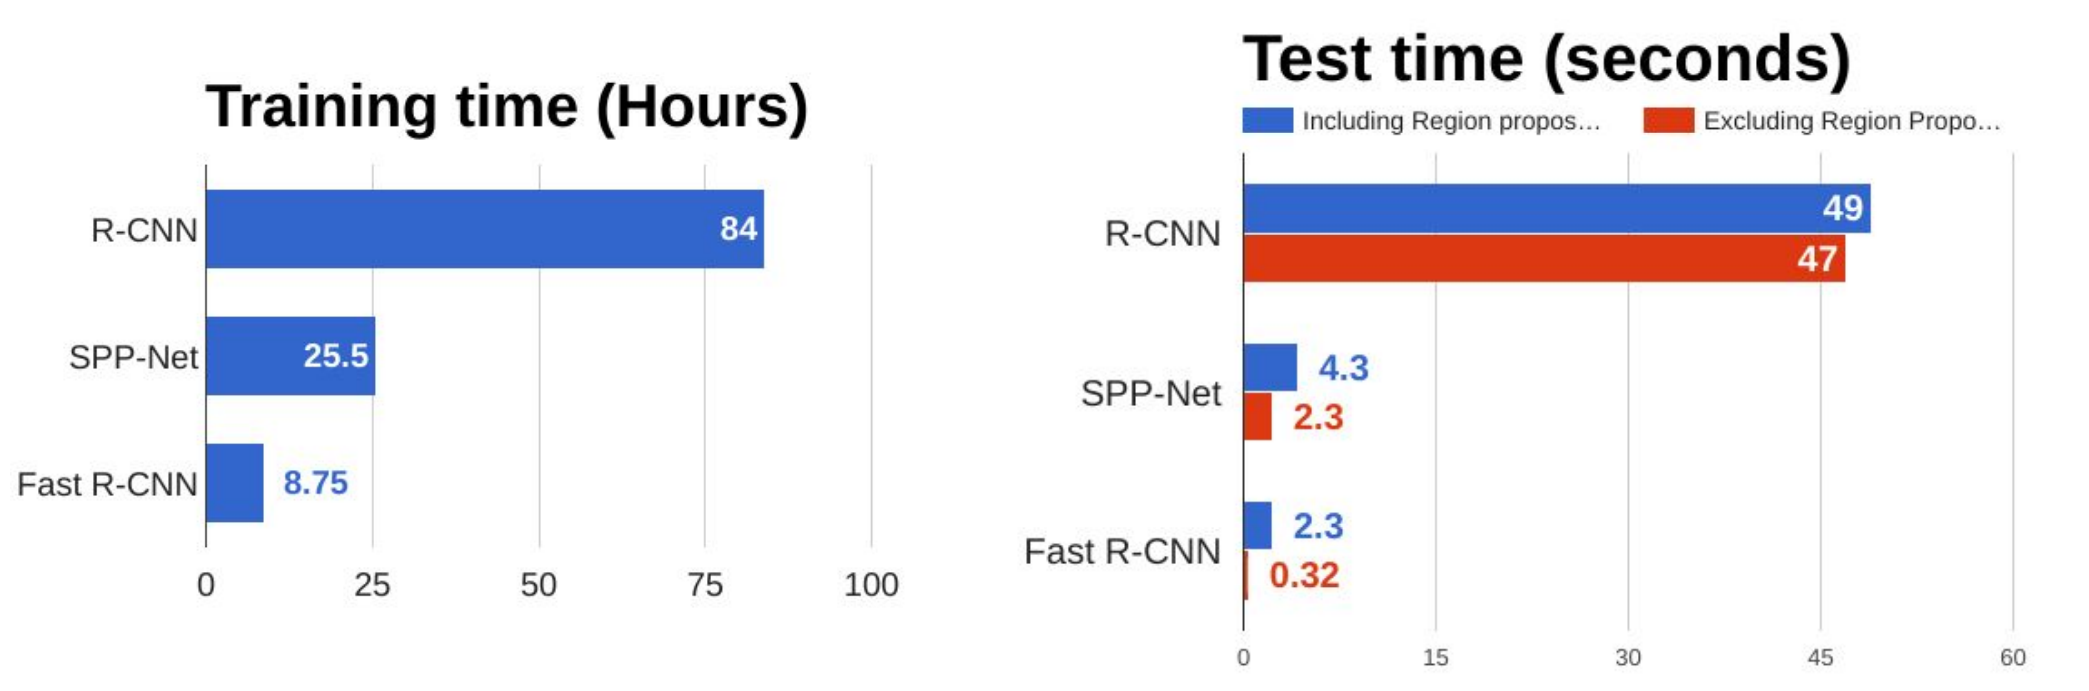
\includegraphics[width=1.0\textwidth,height=1.0\textheight,keepaspectratio]{./images/fast_rcnn_2.png}
\end{figure}

\framebreak

\begin{figure}
\centering
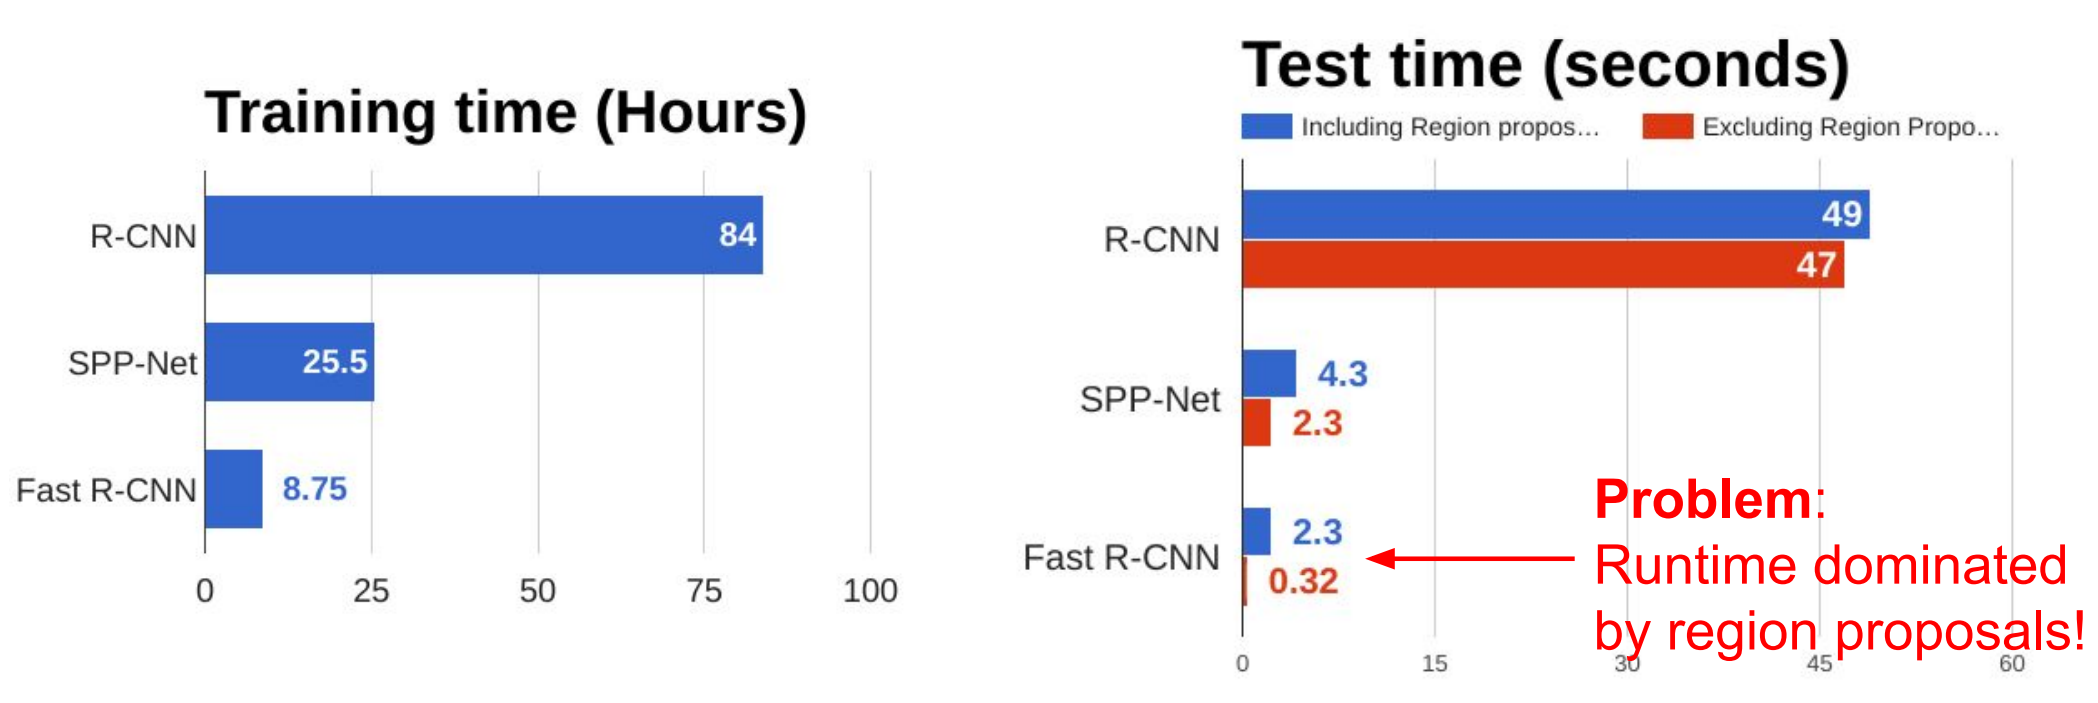
\includegraphics[width=1.0\textwidth,height=1.0\textheight,keepaspectratio]{./images/fast_rcnn_3.png}
\end{figure}
    
\end{frame}

\begin{frame}{Faster R-CNN}
\begin{itemize}
    \item Make CNN do proposals!
    \item Insert Region Proposal Network (RPN) to predict proposals from features
    \pause
    \item Jointly train on 4 losses:
    \begin{itemize}
        \item \textbf{RPN classification:} anchor box is object / not an object
        \item \textbf{RPN regression:} predict transform from anchor box to proposal box
        \item \textbf{Object classification:} classify proposals as background / object class
        \item \textbf{Object regression:} predict transform from proposal box to object box
    \end{itemize}
\end{itemize}
    
\end{frame}

\begin{frame}[allowframebreaks]{Faster R-CNN}
\begin{figure}
\centering
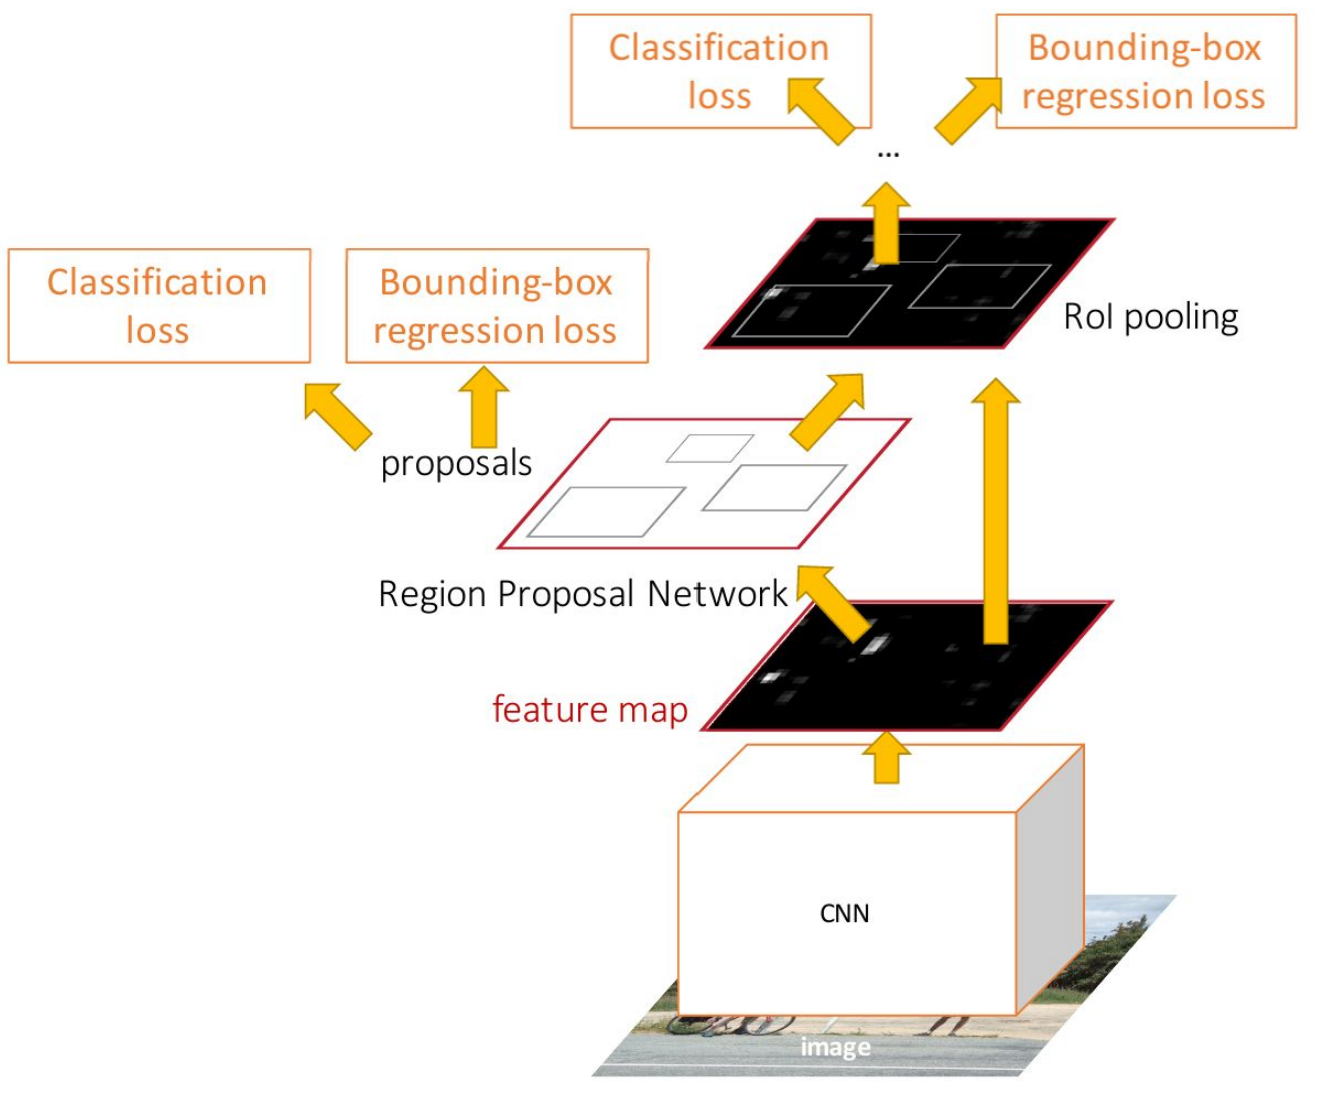
\includegraphics[width=1.0\textwidth,height=0.9\textheight,keepaspectratio]{./images/faster_rcnn_1.png}
\end{figure}

\framebreak

\begin{figure}
\centering
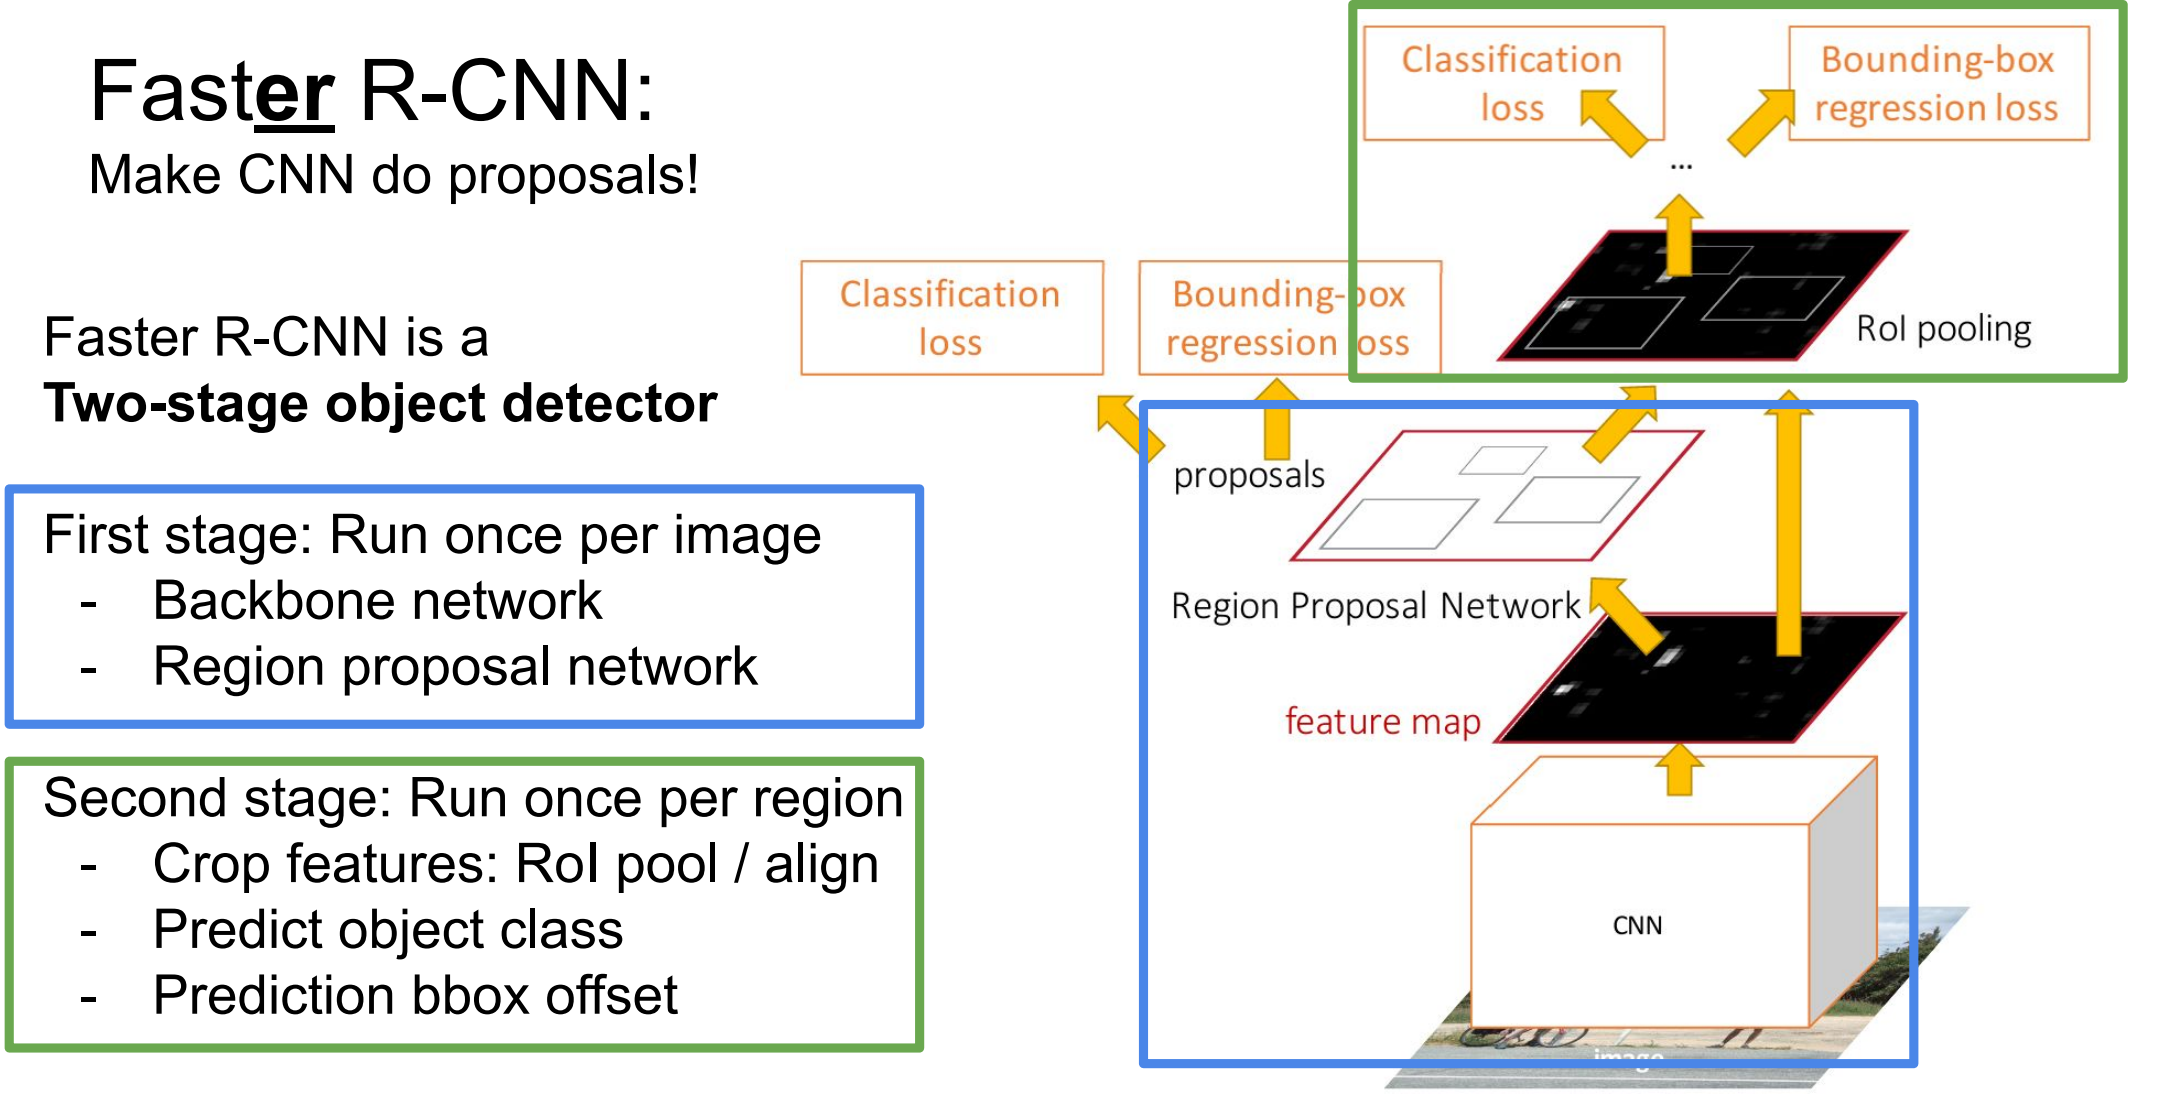
\includegraphics[width=1.0\textwidth,height=1.0\textheight,keepaspectratio]{./images/faster_rcnn_2.png}
\end{figure}

\framebreak

\begin{figure}
\centering
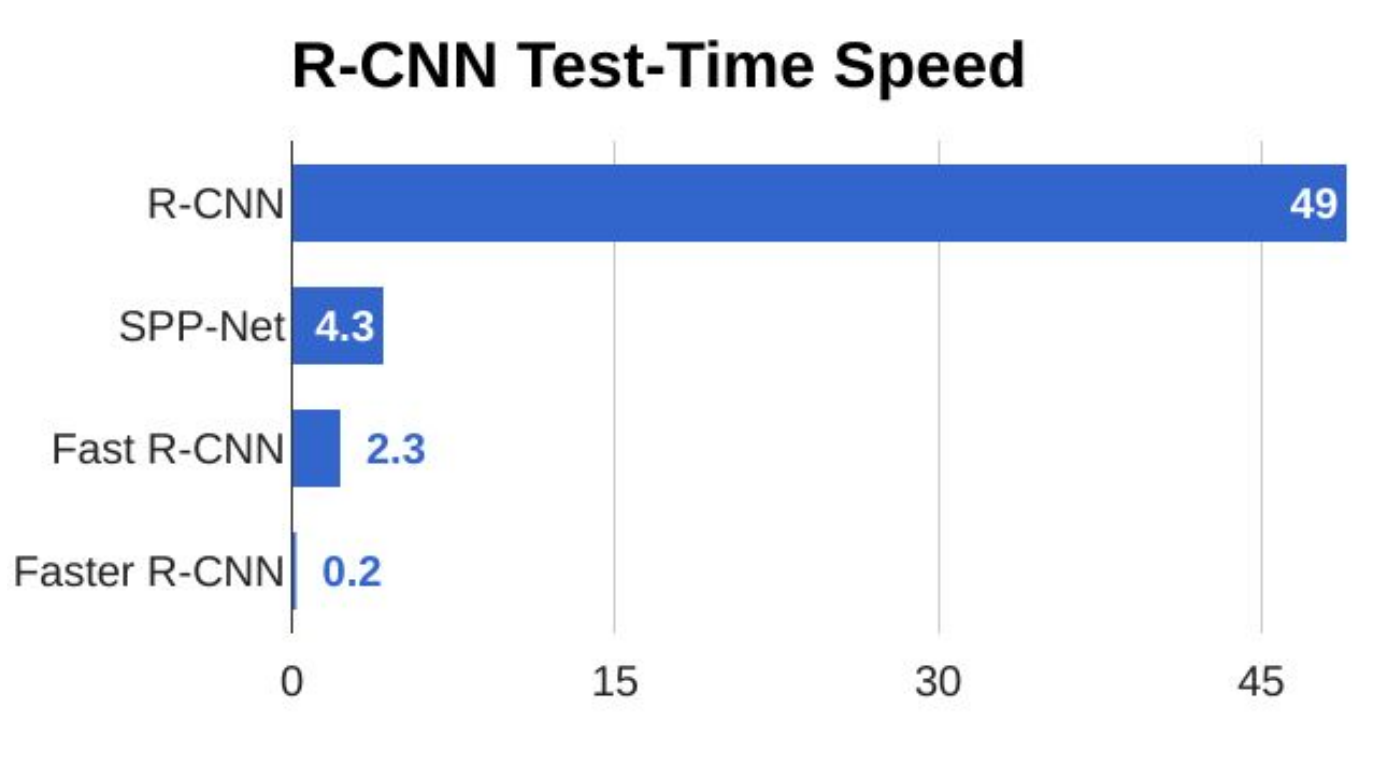
\includegraphics[width=1.0\textwidth,height=1.0\textheight,keepaspectratio]{./images/faster_rcnn_3.png}
\end{figure}
\end{frame}

\begin{frame}{Dealing with Scale}
\begin{itemize}
    \item We need to detect objects of many different scales.
    \item How to improve scale invariance of the detector
\end{itemize}

\begin{figure}
\centering
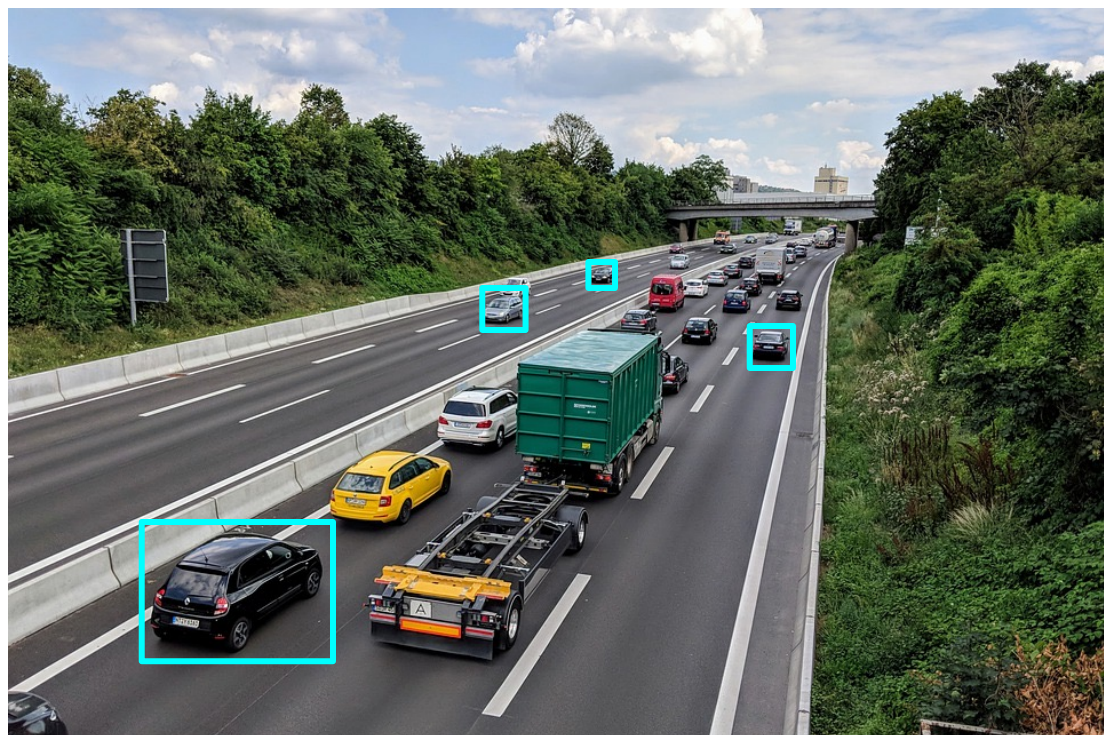
\includegraphics[width=1.0\textwidth,height=0.7\textheight,keepaspectratio]{./images/scale_1.png}
\end{figure}
    
\end{frame}

\begin{frame}[allowframebreaks]{Dealing with Scale: Image Pyramid}
\begin{figure}
\centering
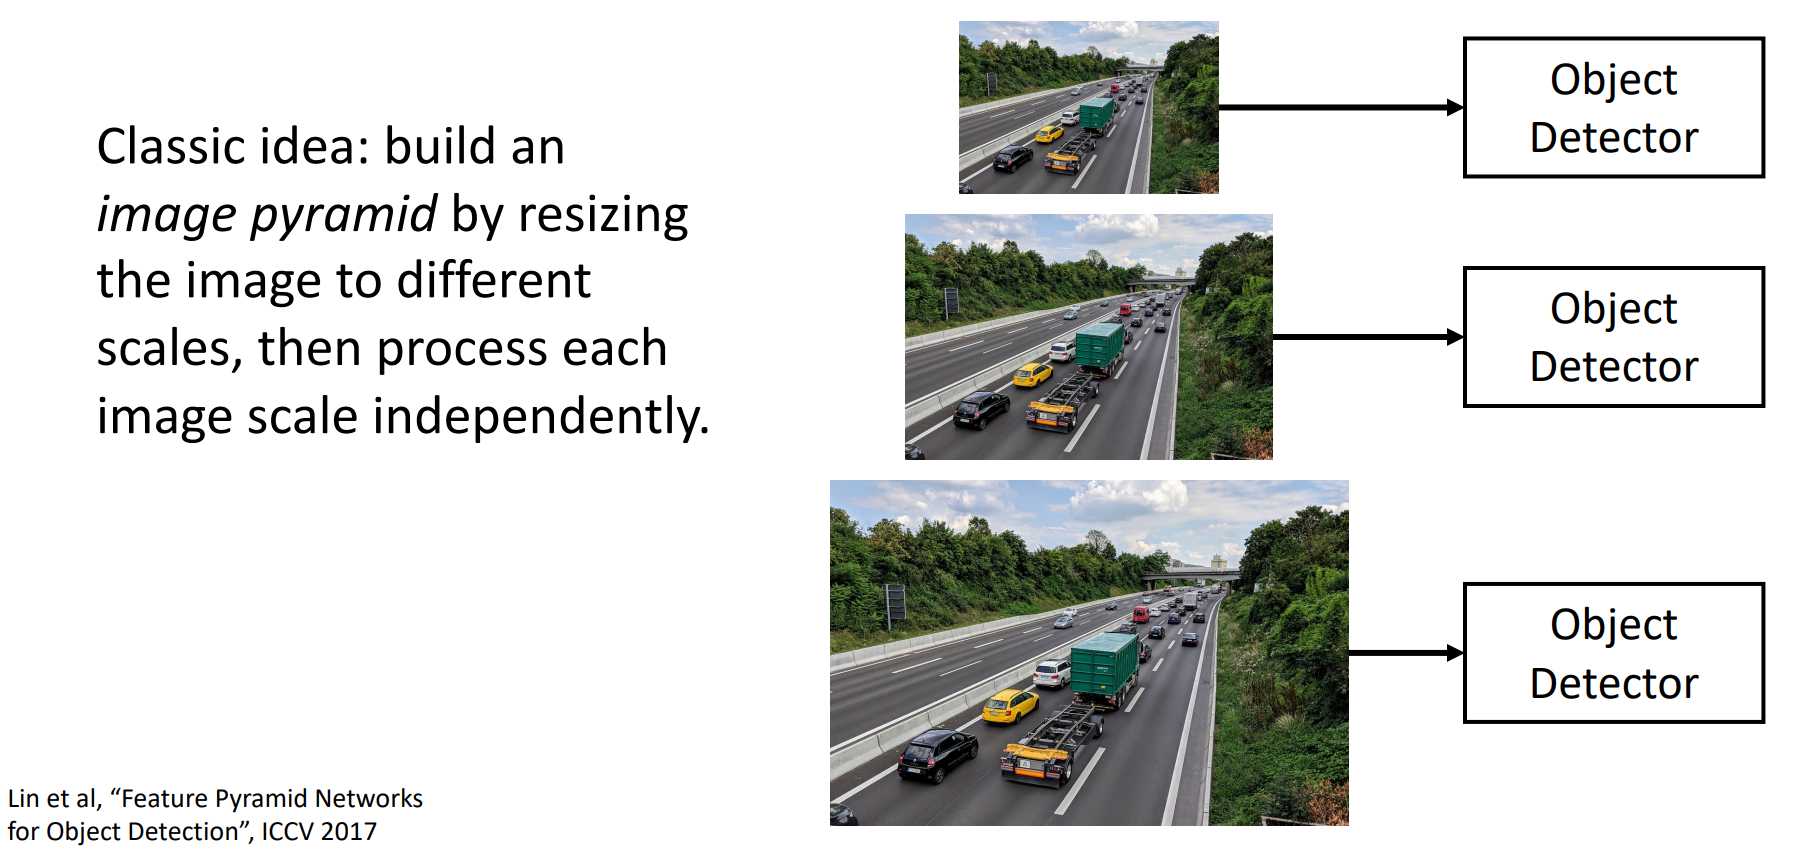
\includegraphics[width=1.0\textwidth,height=1.0\textheight,keepaspectratio]{./images/scale_2.png}
\end{figure}

\framebreak

\begin{figure}
\centering
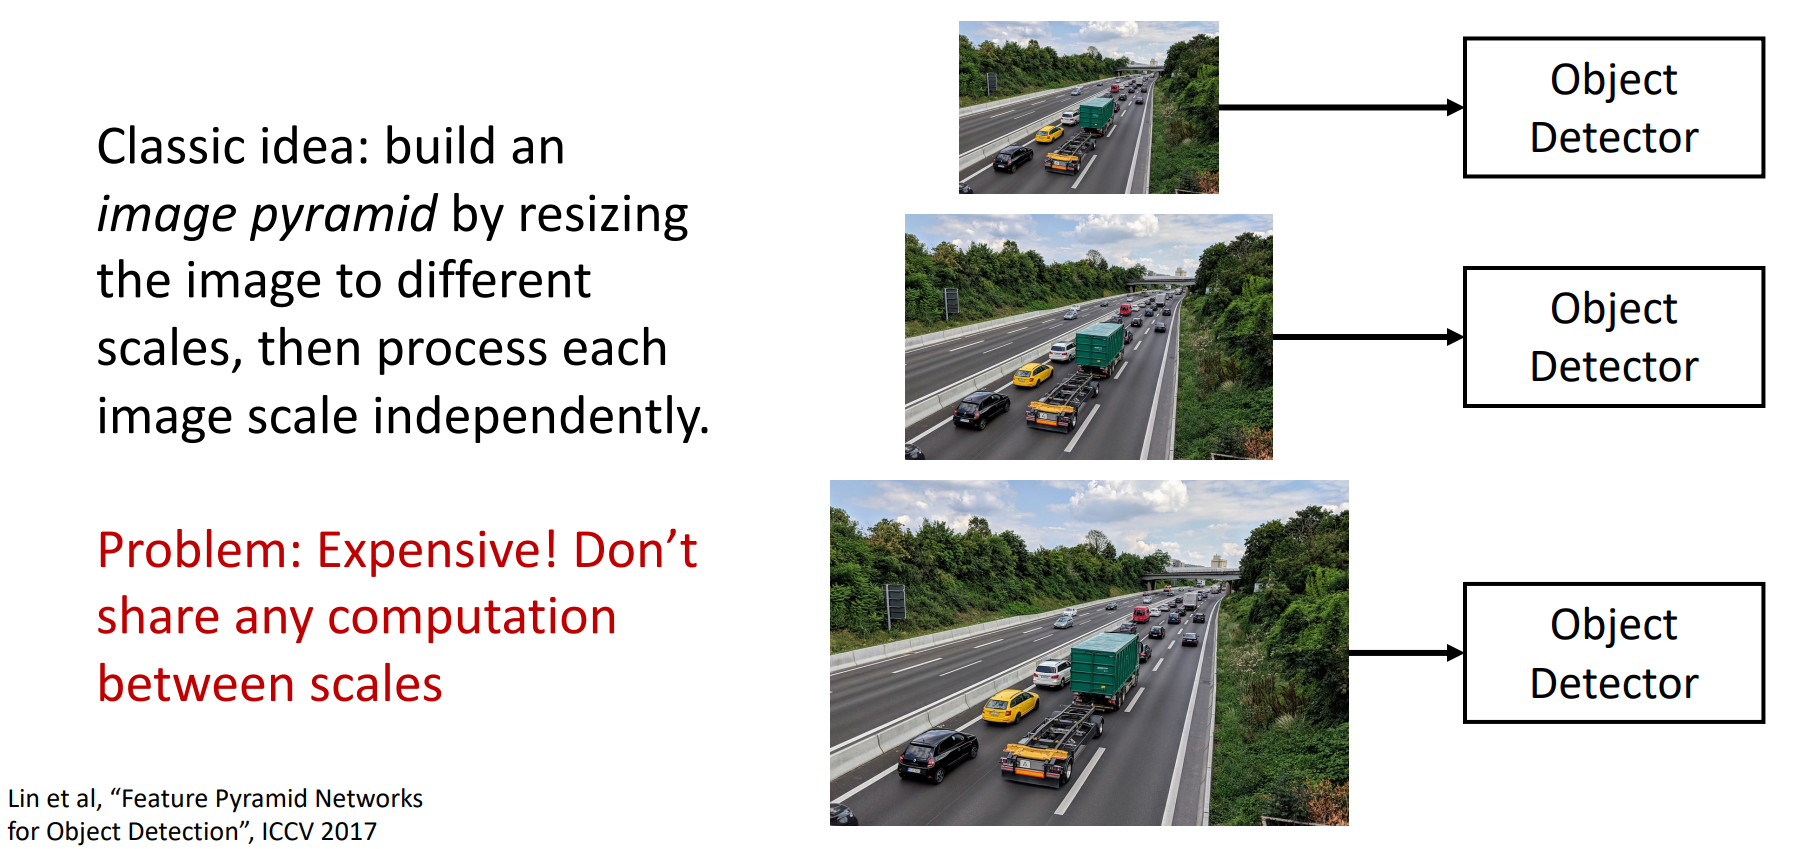
\includegraphics[width=1.0\textwidth,height=1.0\textheight,keepaspectratio]{./images/scale_3.png}
\end{figure}
    
\end{frame}

\begin{frame}[allowframebreaks]{Dealing with Scale: Image Pyramid}
\begin{figure}
\centering
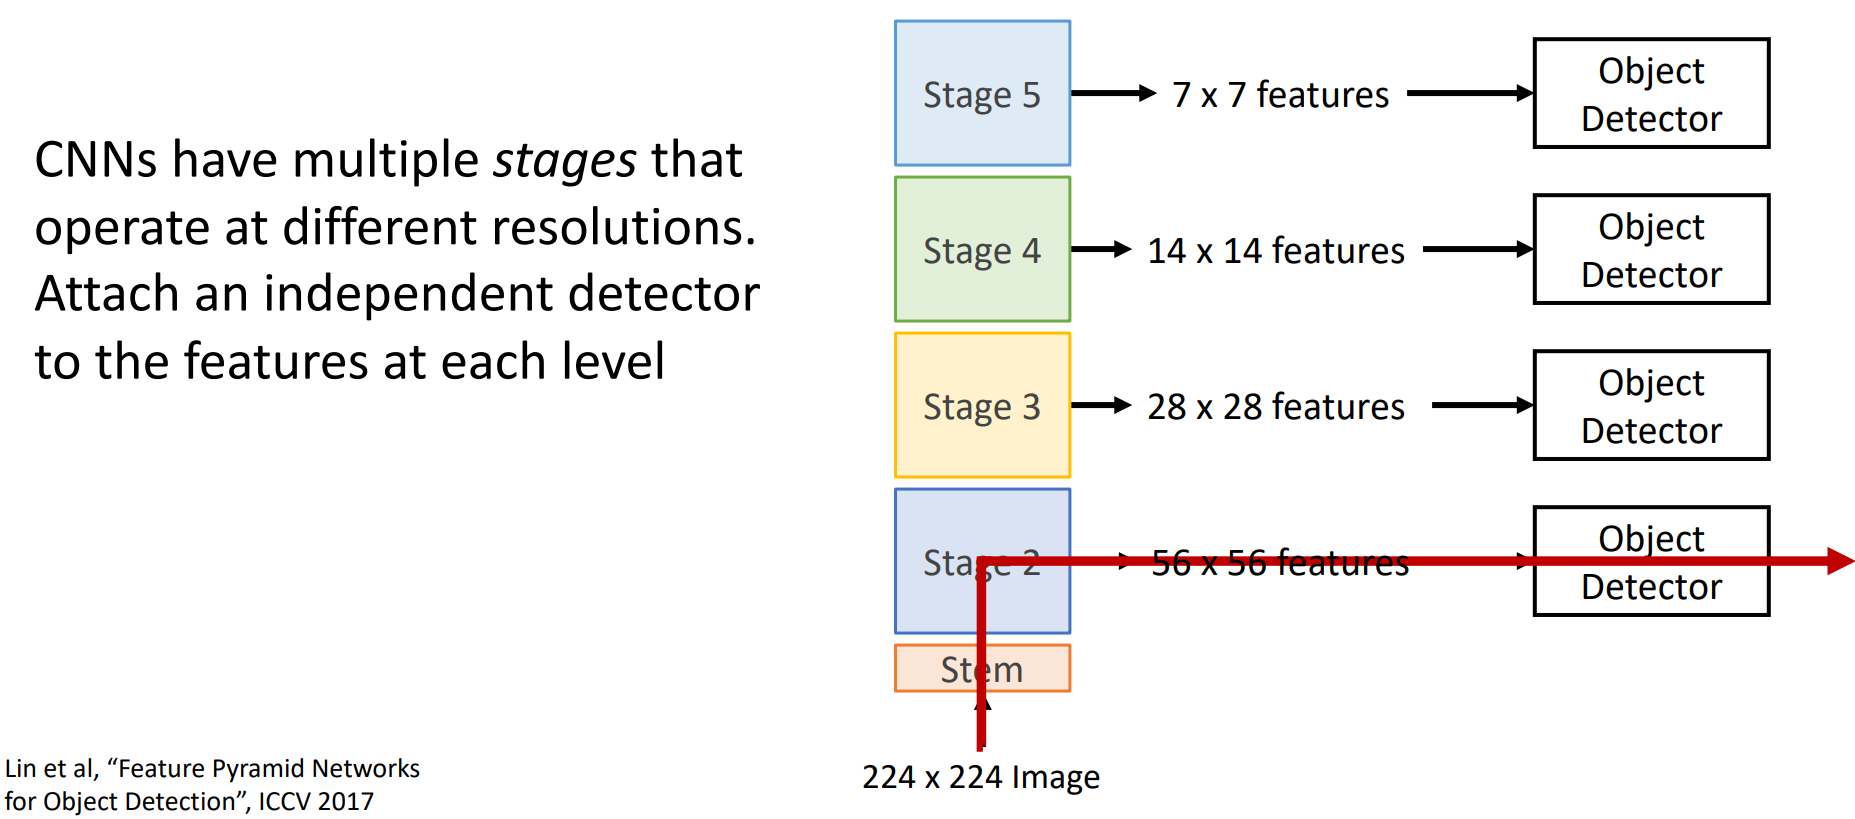
\includegraphics[width=1.0\textwidth,height=1.0\textheight,keepaspectratio]{./images/scale_4.png}
\end{figure}

\framebreak

\begin{figure}
\centering
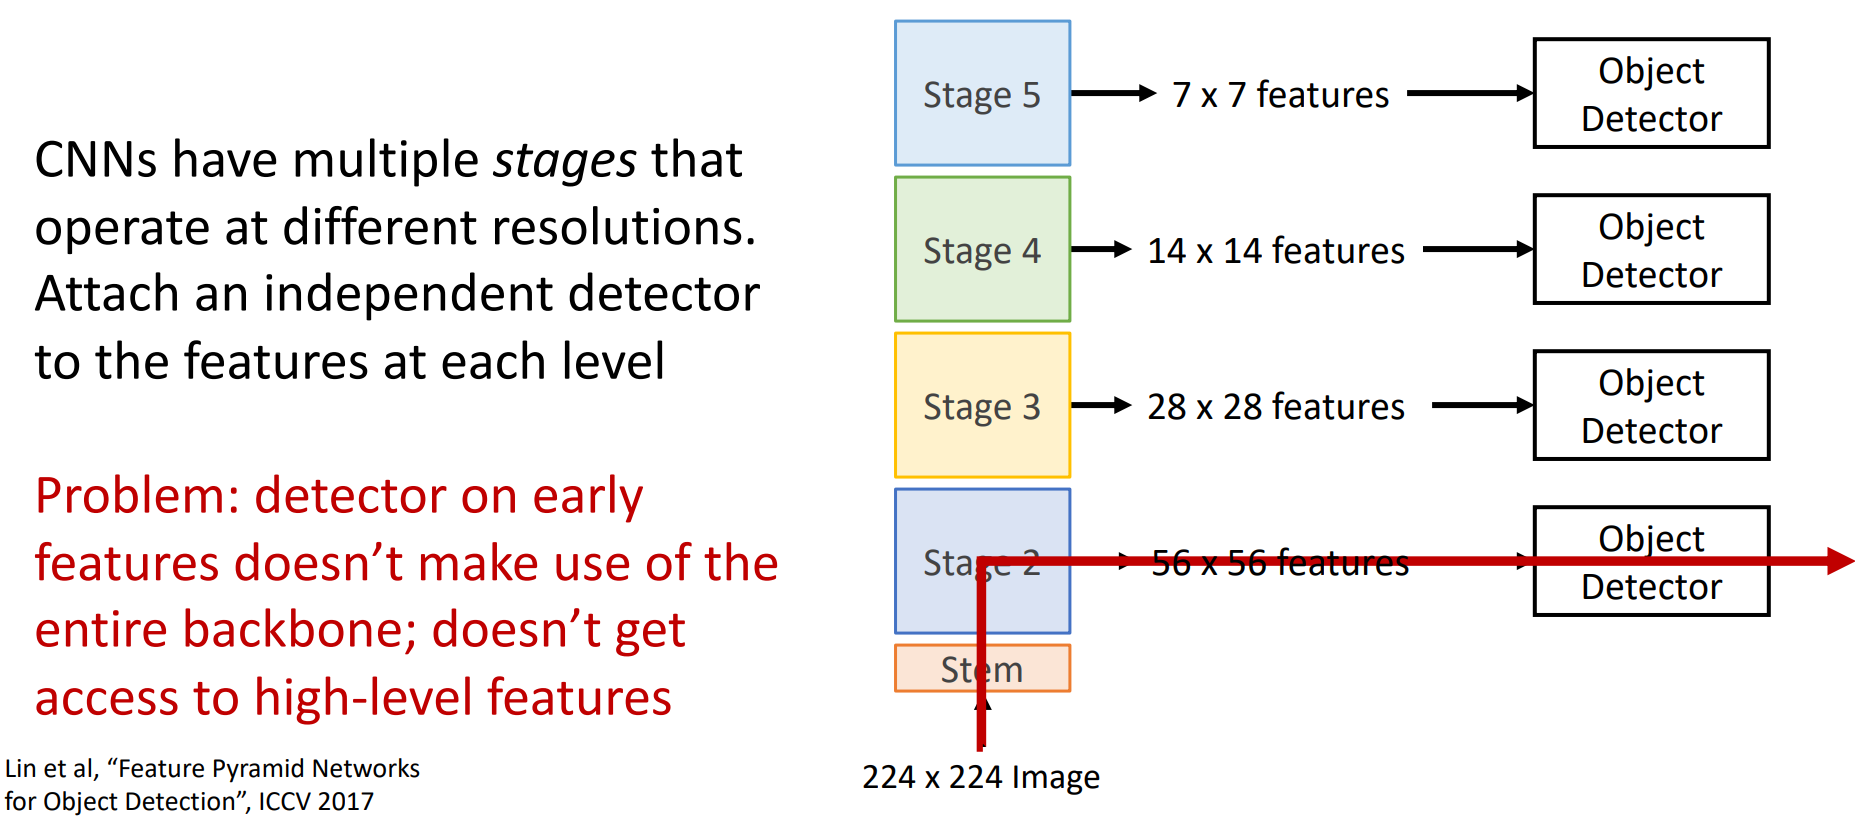
\includegraphics[width=1.0\textwidth,height=1.0\textheight,keepaspectratio]{./images/scale_5.png}
\end{figure}
    
\end{frame}

\begin{frame}[allowframebreaks]{Dealing with Scale: Feature Pyramid Network}
\begin{figure}
\centering
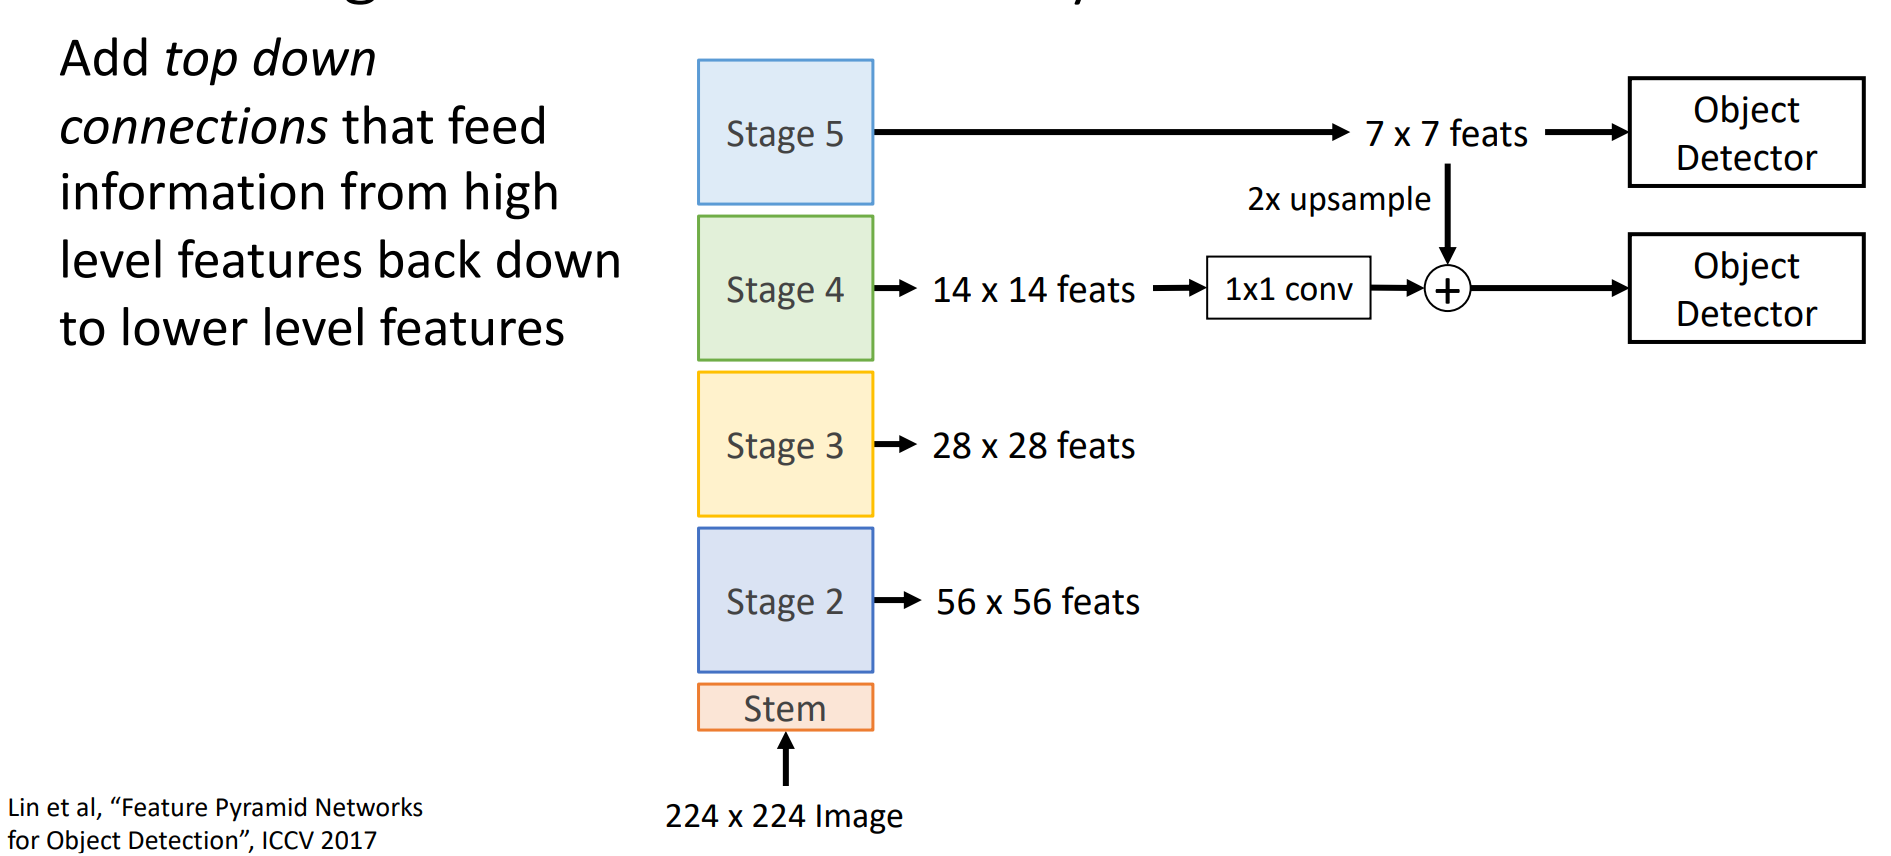
\includegraphics[width=1.0\textwidth,height=1.0\textheight,keepaspectratio]{./images/scale_6.png}
\end{figure}

\framebreak

\begin{figure}
\centering
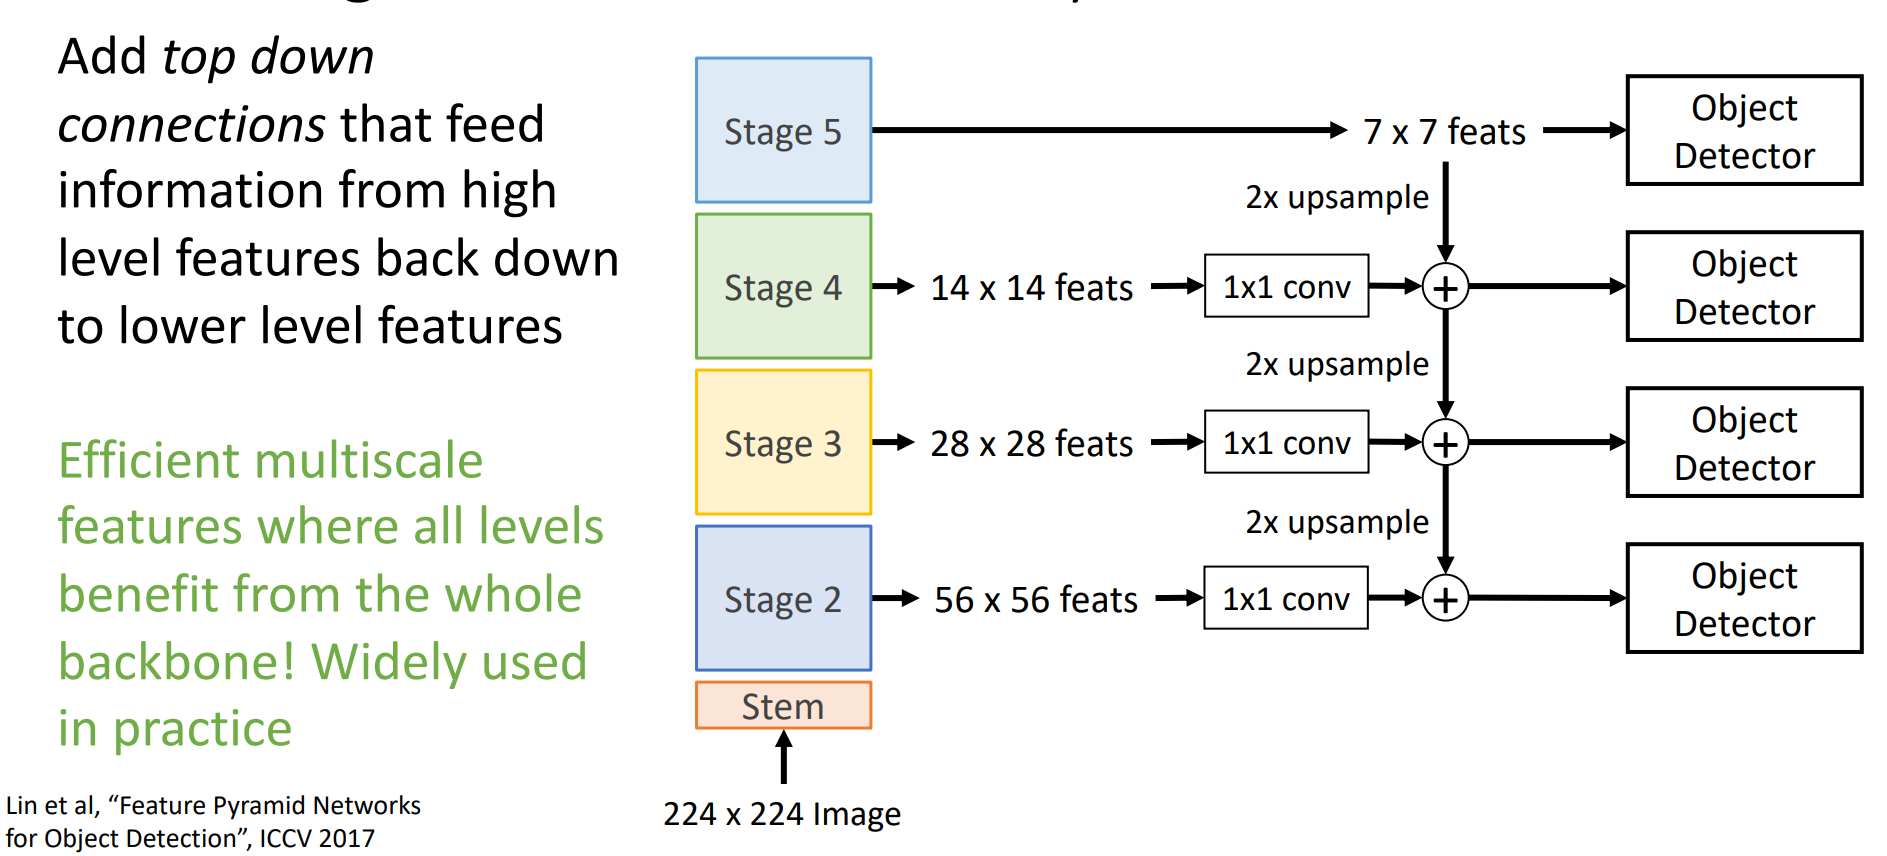
\includegraphics[width=1.0\textwidth,height=1.0\textheight,keepaspectratio]{./images/scale_7.png}
\end{figure}

\framebreak

\begin{figure}
\centering
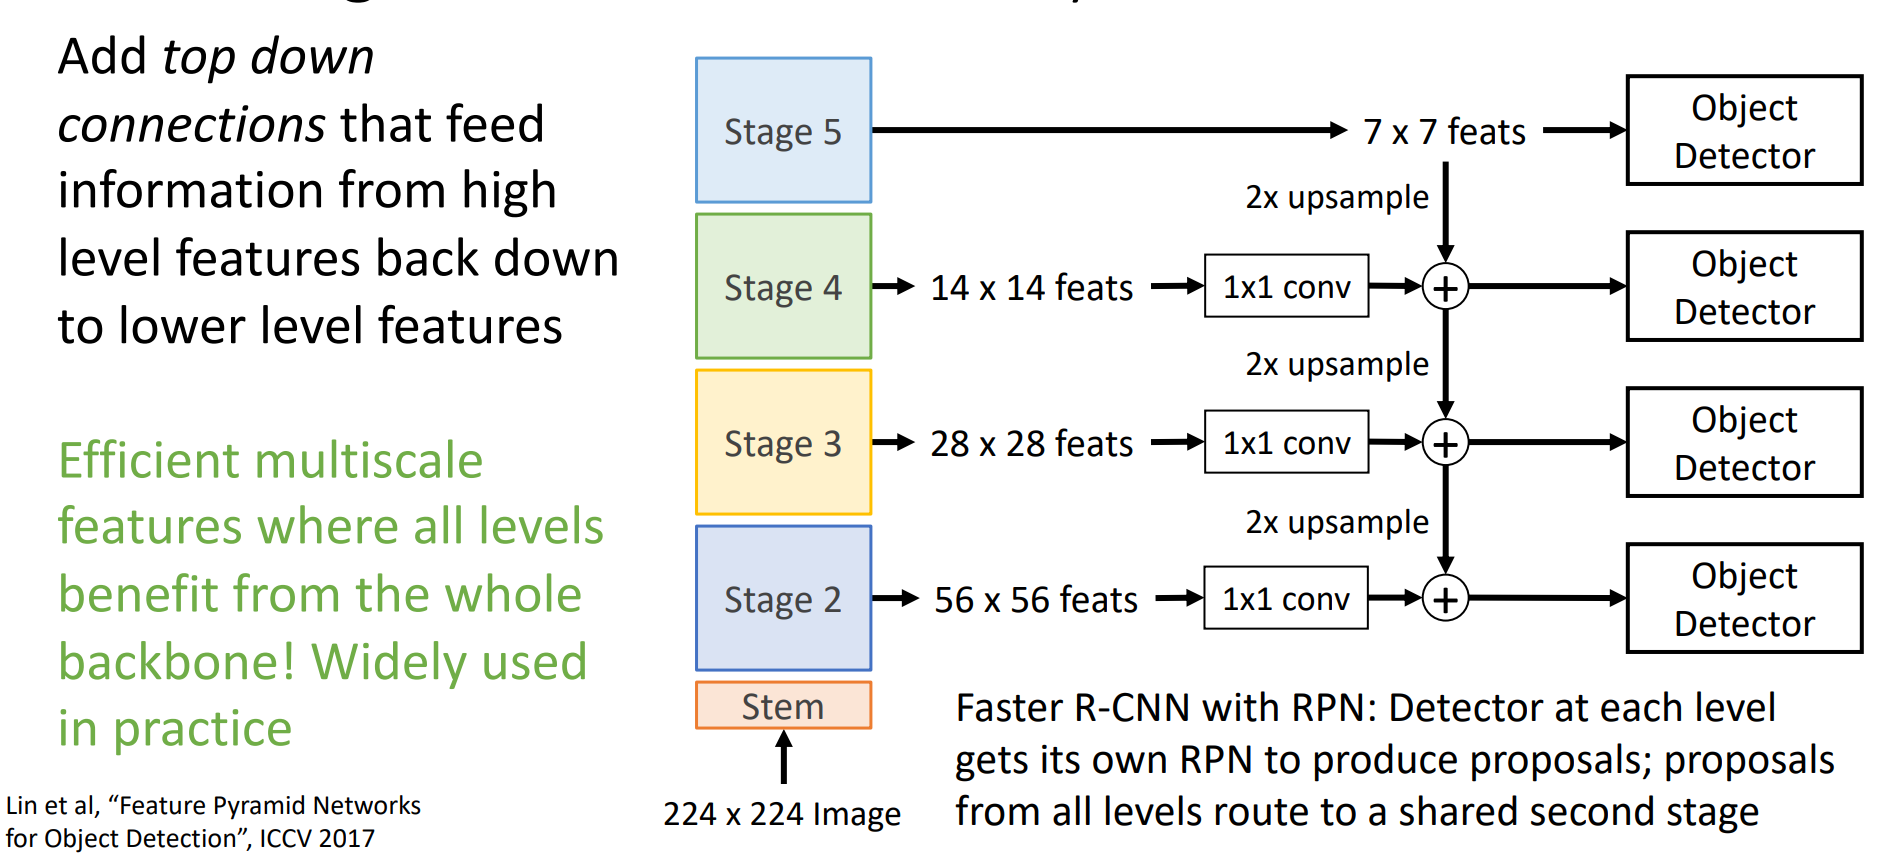
\includegraphics[width=1.0\textwidth,height=1.0\textheight,keepaspectratio]{./images/scale_8.png}
\end{figure}
    
\end{frame}


\begin{frame}{Overlapping Boxes: Non-Max Suppression (NMS)}
\begin{columns}
    \begin{column}{0.5\textwidth}
    \begin{itemize}
        \item<1-> \textbf{Problem:} Object detectors often output many overlapping detections
        \item<2-> \textbf{Solution:} Post-process raw detections using Non-Max Suppression (NMS)
        \onslide<3->{
        \begin{enumerate}
            \item Select next highest-scoring box
            \item Eliminate lower-scoring boxes 
            \item with IoU $>$ threshold (e.g. 0.7)
            \item If any boxes remain, GOTO 1
        \end{enumerate}
        }
        \item<5-> \textcolor{red}{\textbf{Problem:} NMS may eliminate "good" boxes when objects are highly overlapping… no good solution =( }
    \end{itemize}
    \end{column}
    
    \begin{column}{0.5\textwidth}
    \only<-3>{
    \begin{figure}
    \centering
    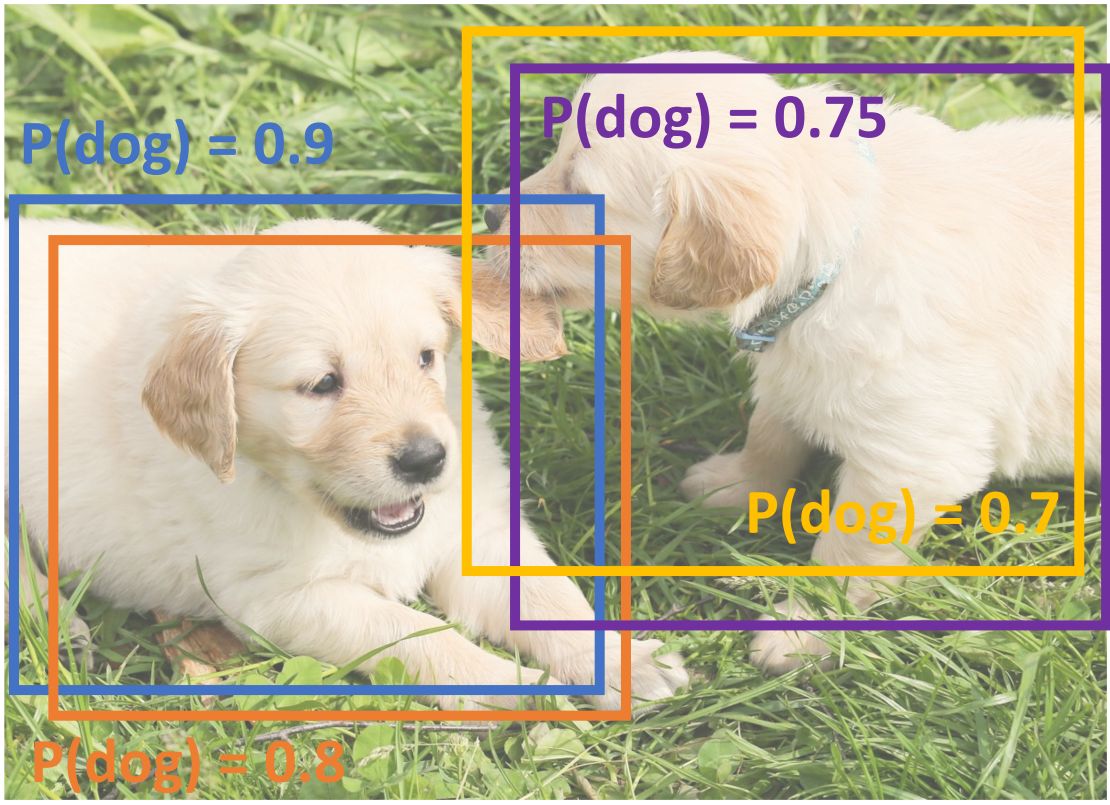
\includegraphics[width=1.0\textwidth,height=1.0\textheight,keepaspectratio]{./images/nms_1.png}
    \end{figure}
    }

    \only<4>{
    \begin{figure}
    \centering
    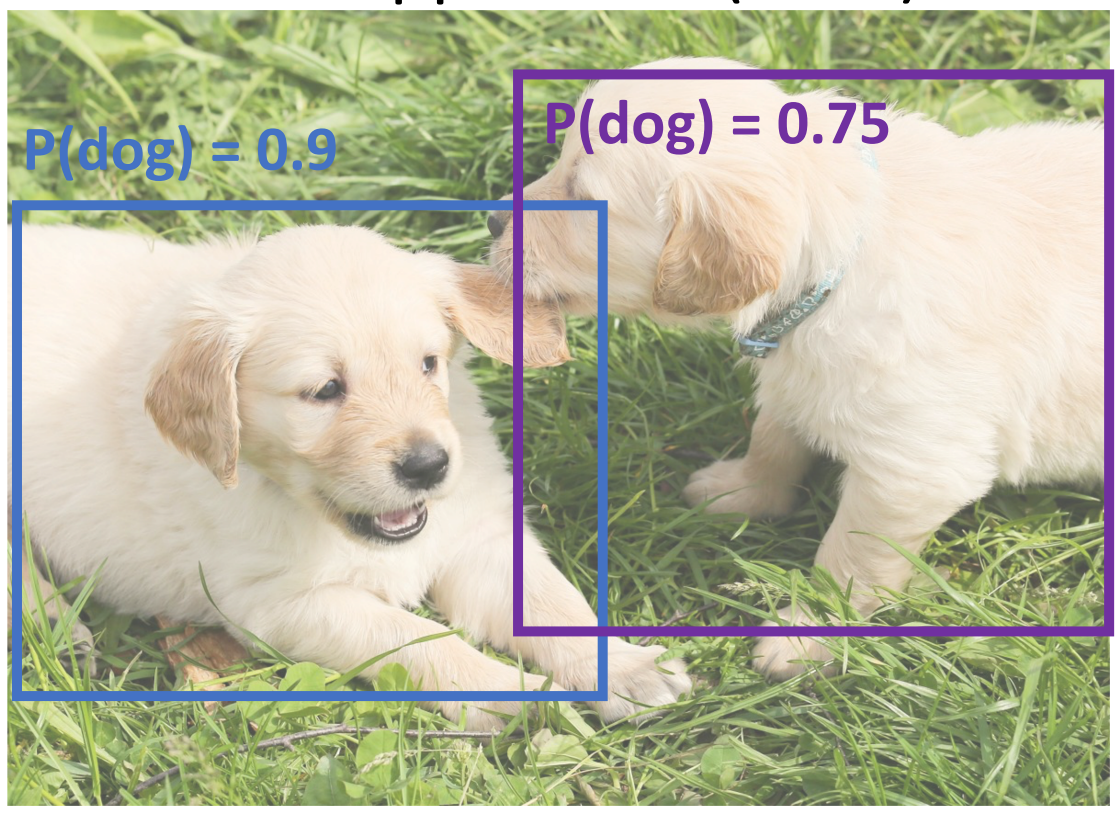
\includegraphics[width=1.0\textwidth,height=1.0\textheight,keepaspectratio]{./images/nms_2.png}
    \end{figure}
    }

    \only<5>{
    \begin{figure}
    \centering
    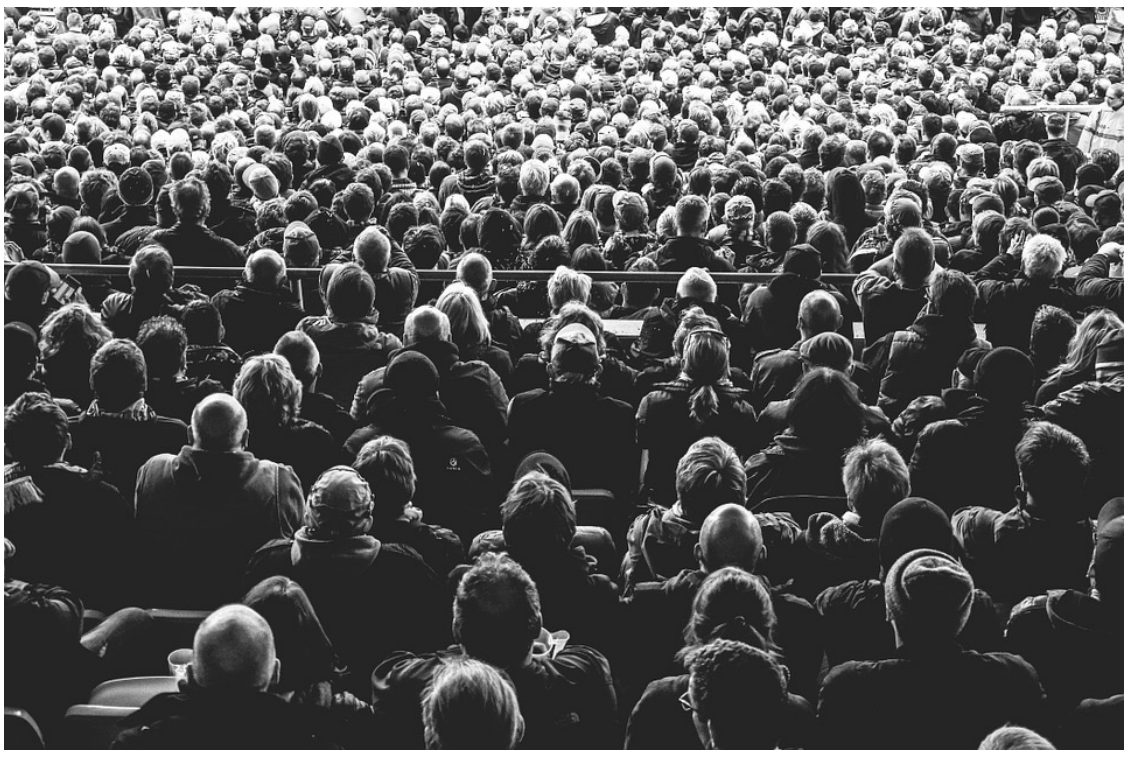
\includegraphics[width=1.0\textwidth,height=1.0\textheight,keepaspectratio]{./images/nms_3.png}
    \end{figure}
    }
        
    \end{column}
\end{columns}
    
\end{frame}

\begin{frame}{Single Shot Object Detection}
\begin{figure}
\centering
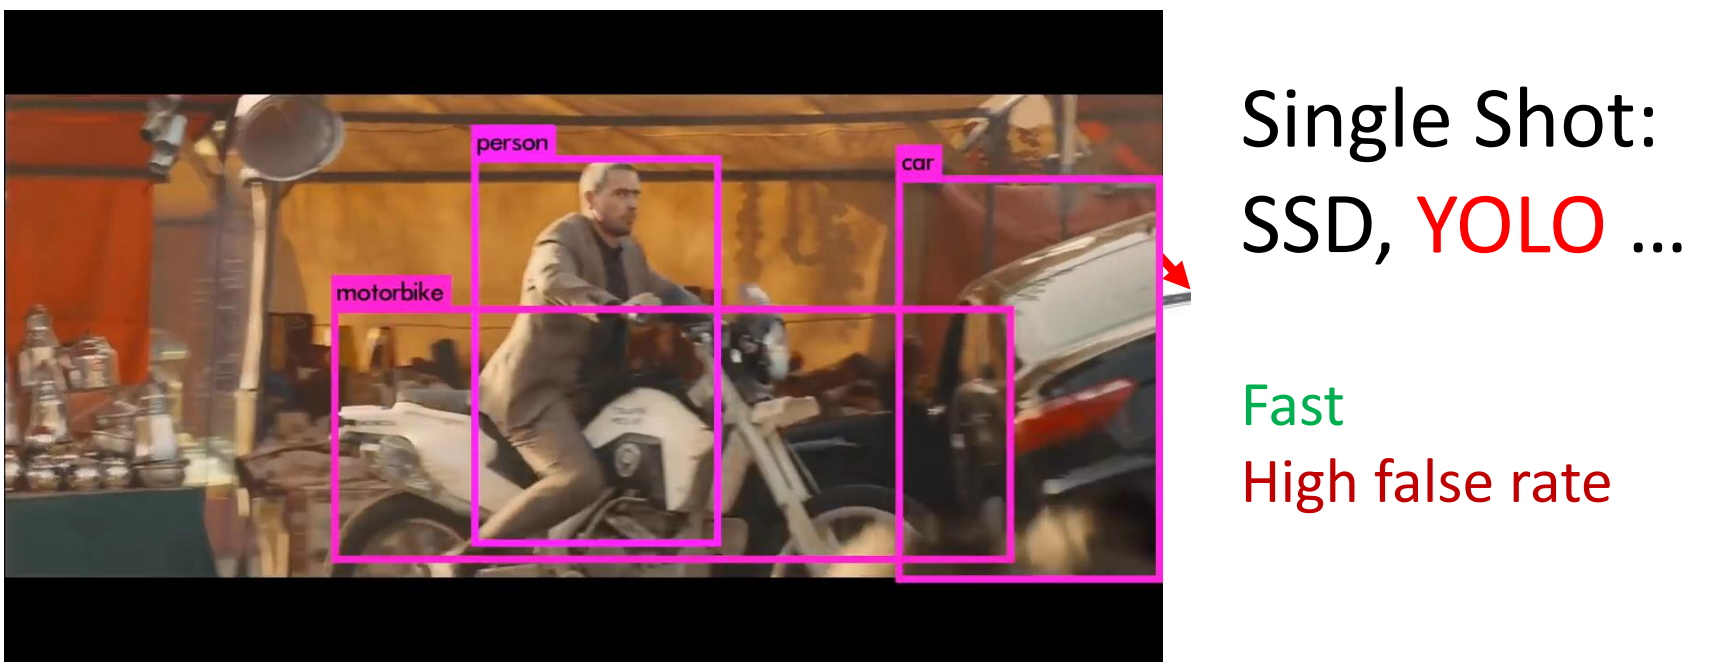
\includegraphics[width=1.0\textwidth,height=1.0\textheight,keepaspectratio]{./images/yolo_1.png}
\end{figure}
    
\end{frame}

\begin{frame}{YOLO - Overview}
\only<1>{
\begin{figure}
\centering
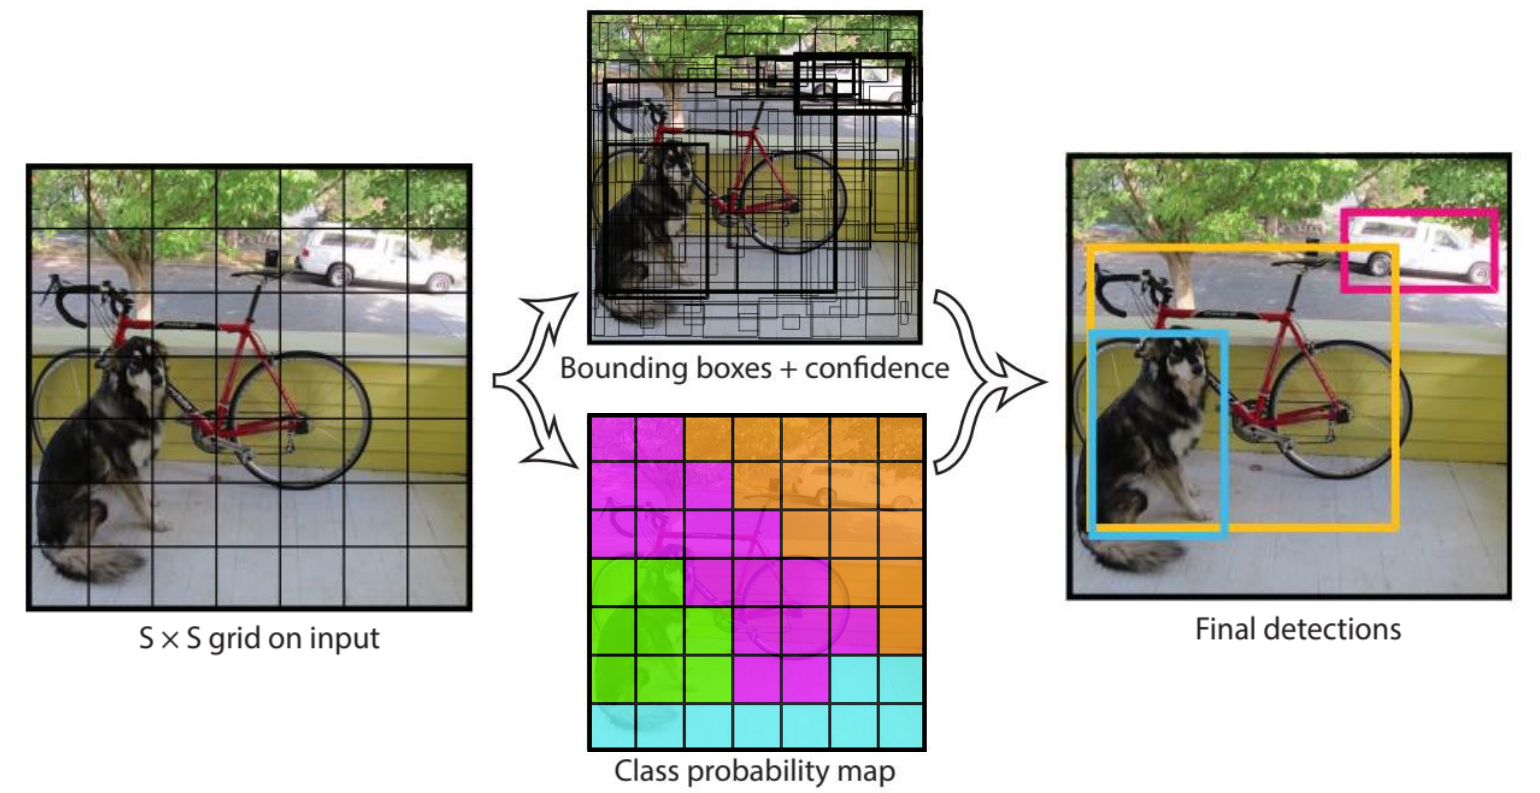
\includegraphics[width=1.0\textwidth,height=1.0\textheight,keepaspectratio]{./images/yolo_2.png}
\end{figure}
}

\only<2>{
\begin{figure}
\centering
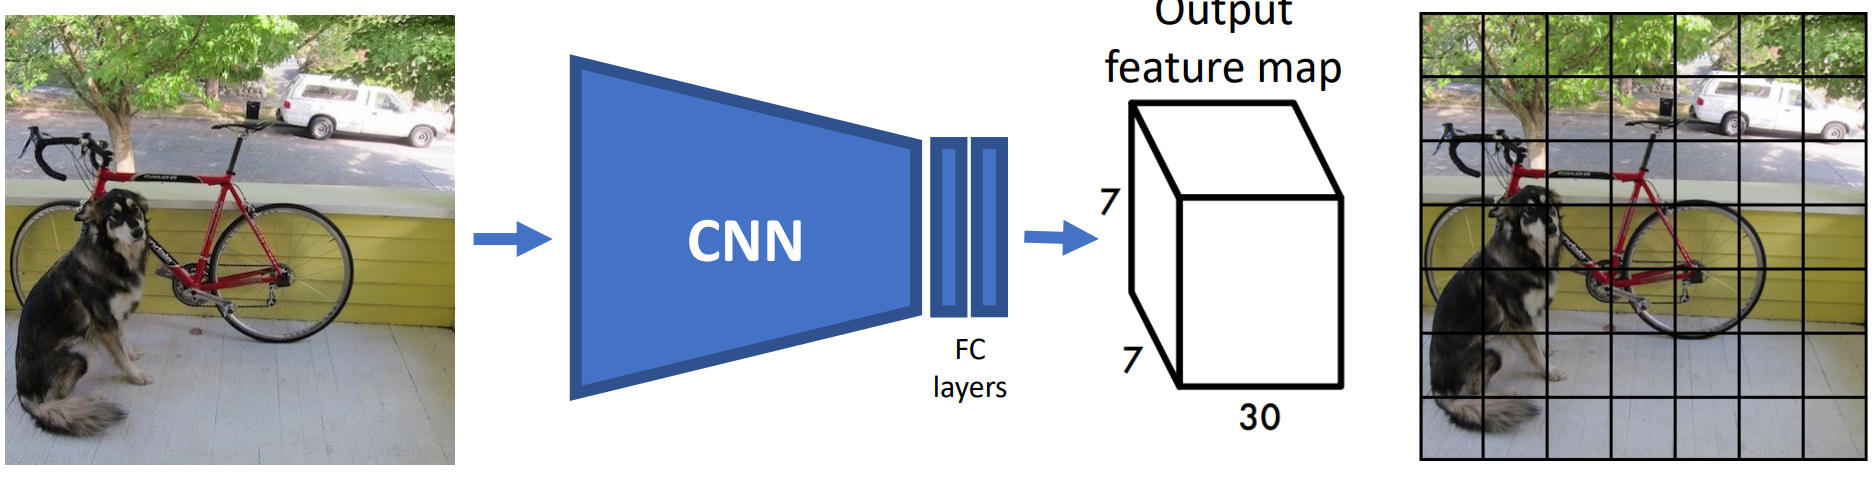
\includegraphics[width=1.0\textwidth,height=1.0\textheight,keepaspectratio]{./images/yolo_3.png}
\end{figure}
}
\only<3>{
\begin{figure}
\centering
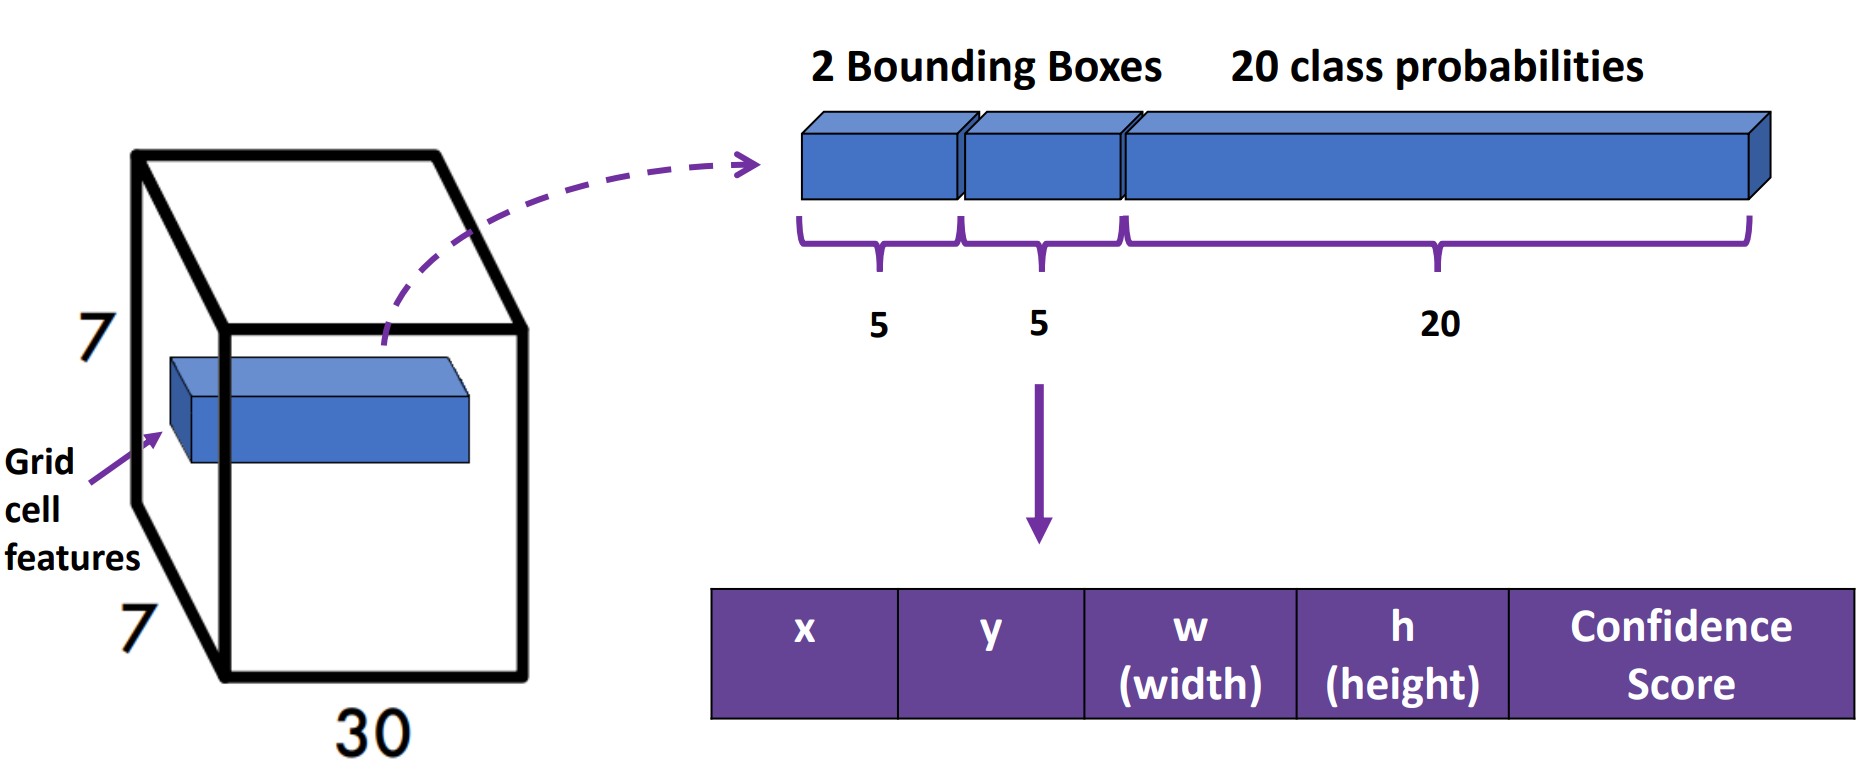
\includegraphics[width=1.0\textwidth,height=1.0\textheight,keepaspectratio]{./images/yolo_4.png}
\end{figure}
}
    
\end{frame}

\begin{frame}{YOLO}
\begin{columns}
    \begin{column}{0.5\textwidth}
    \onslide<2->{Each cell predicts}
    \begin{itemize}
        \item<3-> $B=2$ bounding boxes $(x,y,w,h) + $ confidence score
        \item<4-> $C=20$ class probabilities
        \vspace{1cm}
        \item<8-> Apply Non-Maximum Suppression
    \end{itemize}
    \end{column}
    
    \begin{column}{0.5\textwidth}
    \only<-2>{
    \begin{figure}
    \centering
    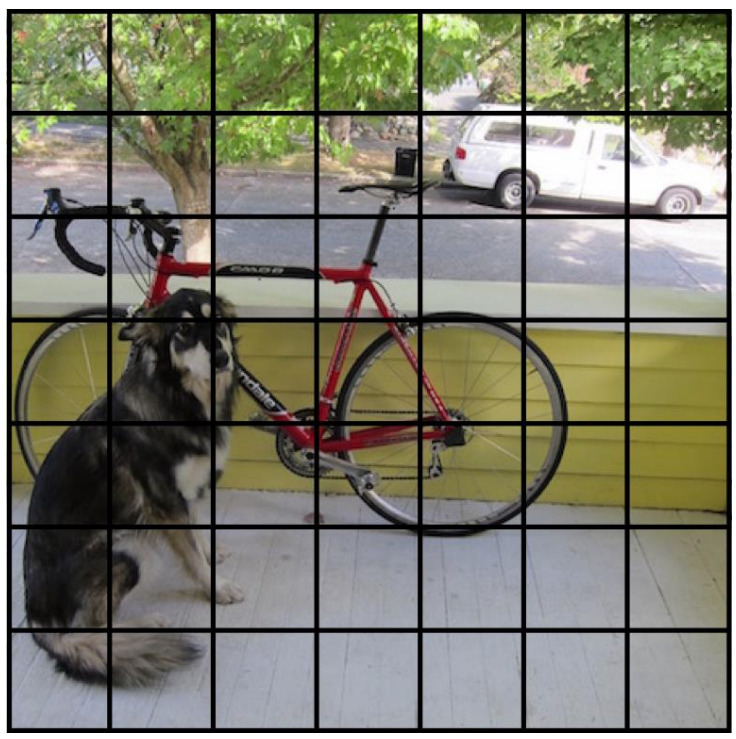
\includegraphics[width=1.0\textwidth,height=1.0\textheight,keepaspectratio]{./images/yolo_5.png}
    \end{figure}
    }

    \only<3-4>{
    \begin{figure}
    \centering
    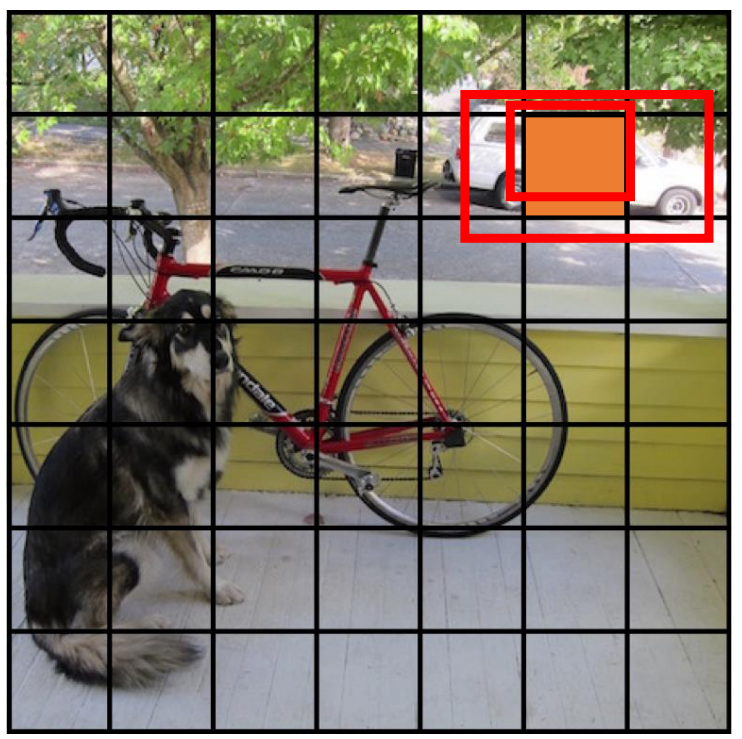
\includegraphics[width=1.0\textwidth,height=1.0\textheight,keepaspectratio]{./images/yolo_6.png}
    \end{figure}
    }

    \only<5>{
    \begin{figure}
    \centering
    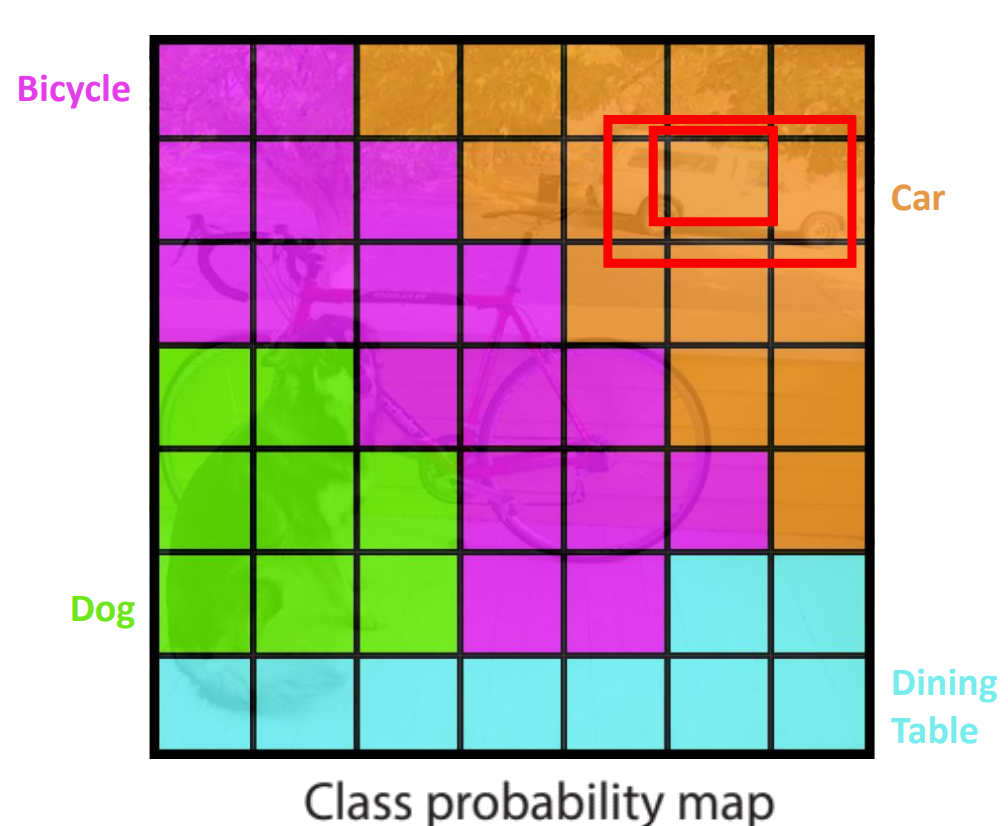
\includegraphics[width=1.0\textwidth,height=1.0\textheight,keepaspectratio]{./images/yolo_7.png}
    \end{figure}
    }

    \only<6>{
    \begin{figure}
    \centering
    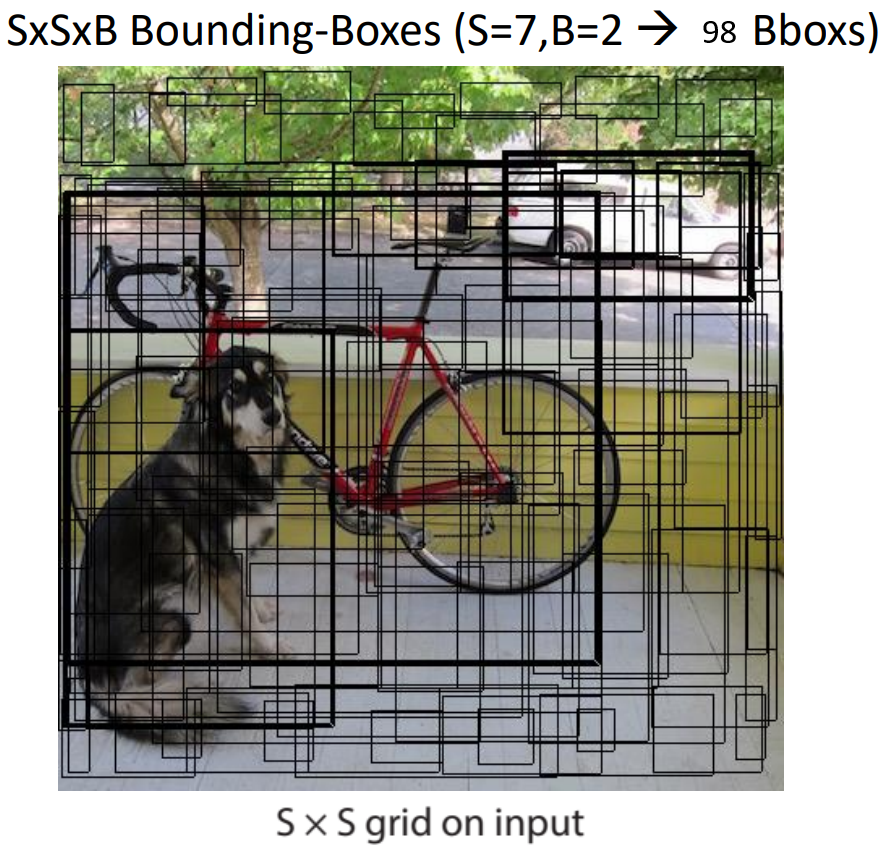
\includegraphics[width=1.0\textwidth,height=1.0\textheight,keepaspectratio]{./images/yolo_8.png}
    \end{figure}
    }

    \only<7>{
    \begin{figure}
    \centering
    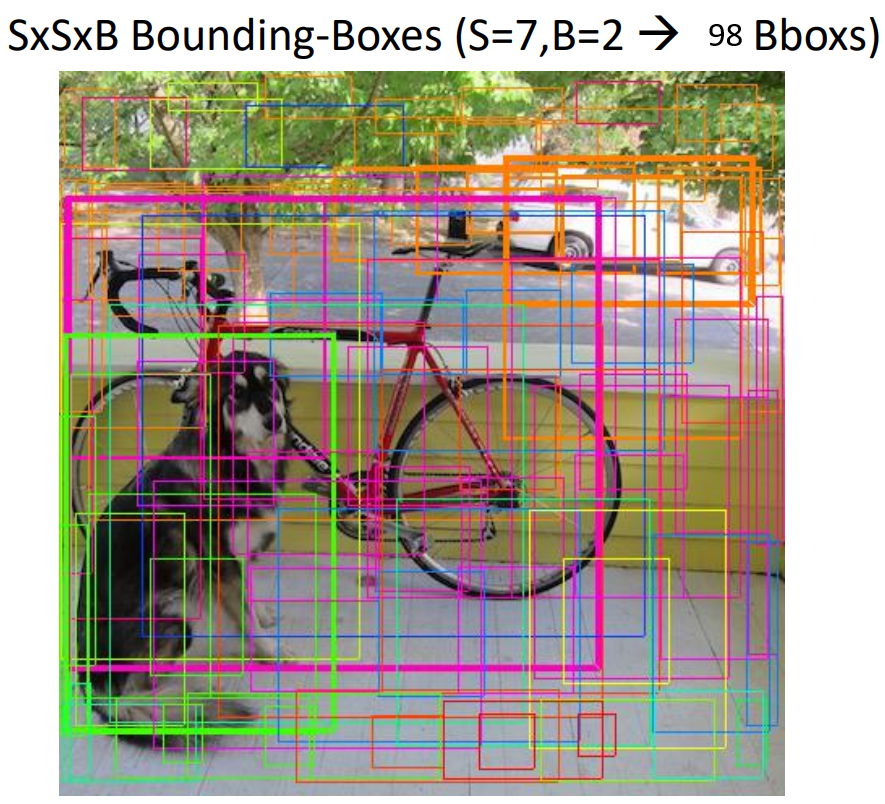
\includegraphics[width=1.0\textwidth,height=1.0\textheight,keepaspectratio]{./images/yolo_9.png}
    \end{figure}
    }

    \only<8>{
    \begin{figure}
    \centering
    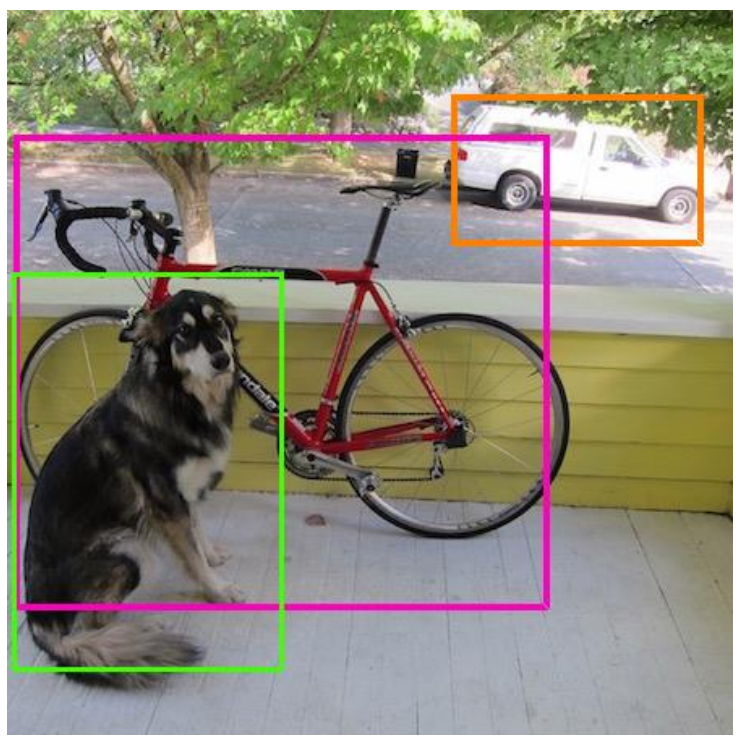
\includegraphics[width=1.0\textwidth,height=1.0\textheight,keepaspectratio]{./images/yolo_10.png}
    \end{figure}
    }
        
    \end{column}
\end{columns}
    
\end{frame}

\begin{frame}{YOLO - Loss Function}
    \begin{figure}
    \centering
    \includegraphics[width=1.0\textwidth,height=1.0\textheight,keepaspectratio]{./images/yolo_11.png}
    \end{figure}
\end{frame}



\begin{frame}{YOLO - Benefits}
\begin{columns}
    \begin{column}{0.6\textwidth}
    \begin{itemize}
        \item Fast. Good for real-time processing
        \item End-to-end training
    \end{itemize}
    \begin{figure}
    \centering
    \includegraphics[width=1.0\textwidth,height=1.0\textheight,keepaspectratio]{./images/yolo_12.png}
    \end{figure}
    
    \end{column}
    
    \begin{column}{0.4\textwidth}
    \begin{figure}
    \centering
    \includegraphics[width=1.0\textwidth,height=0.95\textheight,keepaspectratio]{./images/yolo_13.png}
    \end{figure}
        
    \end{column}
\end{columns}
    
\end{frame}

\begin{frame}{YOLO - Limitations}
\begin{columns}
    \begin{column}{0.5\textwidth}
    \begin{itemize}
        \item<2-> Difficult to detect small objects
        \item<2-> Coarse predictions
        \item<3-> Fixed input size
        \item<4-> A grid cell can predict only one class
        \vspace{0.5cm}
        \onslide<5->{
        \item \textcolor{red}{Solutions:}
        \begin{itemize}
            \item Remove fc layers!
            \item Predict class per bbox (not per cell)
        \end{itemize}
        }
    \end{itemize}
    \end{column}
    
    \begin{column}{0.5\textwidth}
    \only<-2>{
    \begin{figure}
    \centering
    \includegraphics[width=1.0\textwidth,height=1.0\textheight,keepaspectratio]{./images/yolo_14.png}
    \end{figure}
    }

    \only<3>{
    \begin{figure}
    \centering
    \includegraphics[width=1.0\textwidth,height=1.0\textheight,keepaspectratio]{./images/yolo_15.png}
    \end{figure}
    }

    \only<4->{
    \begin{figure}
    \centering
    \includegraphics[width=1.0\textwidth,height=1.0\textheight,keepaspectratio]{./images/yolo_16.png}
    \end{figure}
    }
        
    \end{column}
\end{columns}
\end{frame}

\begin{frame}{YOLOv2}
\begin{itemize}
    \item Removed fully connected layers
    \item A grid cell predicts class probabilities for each box
\end{itemize}
\begin{figure}
\centering
\includegraphics[width=1.0\textwidth,height=1.0\textheight,keepaspectratio]{./images/yolo_17.png}
\end{figure}

    
\end{frame}

\begin{frame}{There's always room for improvement!}
\begin{itemize}
    \item YOLOv3
    \begin{itemize}
        \item J. Redmon, A. Farhadi. Yolov3: An incremental improvement, 2018
    \end{itemize}
    \item YOLOv4
    \begin{itemize}
        \item A. Bochkovskiy, C. Wang, H. Liao. Yolov4: Optimal speed and accuracy of object detection (Feb. 2020)
    \end{itemize}
    \item YOLOv5
    \begin{itemize}
        \item YOLOv5 by ultralytics (June 2020)
    \end{itemize}
    \item PP-YOLO
    \begin{itemize}
        \item X. Long, K. Deng, G. Wang, Y. Zhang, Q. Dang, Y. Gao, H. Shen, J. Ren, S. Han, E. Ding, S. Wen. Pp-yolo: An effective and efficient implementation of object detector (June 2020)
    \end{itemize}
    \item PP-YOLOv2 (2021)
    \begin{itemize}
        \item J. X. Huang, X. Wang, W. Lv, X. Bai, X. Long, K. Deng, Q. Dang, S. Han, Q. Liu, X. Hu, D. Yu, Y. Ma, O. Yoshie. PP-YOLOv2: A Practical Object Detector (2021)
    \end{itemize}

\end{itemize}
    
\end{frame}

\begin{frame}{Things and Stuff}
\begin{columns}
    \begin{column}{0.5\textwidth}
        \begin{itemize}
            \item \textbf{Things:} Object categories that can be separated into object instances (e.g. cats, cars, person)
            \item \textbf{Stuff:} Object categories that cannot be separated into instances (e.g. sky, grass, water, trees)
        \end{itemize}
    \end{column}
    \begin{column}{0.5\textwidth}
        \begin{figure}
        \centering
        \includegraphics[width=1.0\textwidth,height=1.0\textheight,keepaspectratio]{./images/ins_1.png}
        \end{figure}
    \end{column}
\end{columns}
    
\end{frame}

\begin{frame}{Computer Vision Tasks}
\begin{columns}
    \begin{column}{0.5\textwidth}
        \begin{itemize}
            \item \textbf{Object Detection:} Detects individual object instances, but only gives box(Only things!)
        \end{itemize}
        \begin{figure}
        \centering
        \includegraphics[width=1.0\textwidth,height=1.0\textheight,keepaspectratio]{./images/ins_2.png}
        \end{figure}
    \end{column}
    \begin{column}{0.5\textwidth}
        \begin{itemize}
            \item \textbf{Semantic Segmentation:} Gives per-pixel labels, but merges instances (Both things and stuff)
        \end{itemize}
        \begin{figure}
        \centering
        \includegraphics[width=1.0\textwidth,height=1.0\textheight,keepaspectratio]{./images/ins_3.png}
        \end{figure}
    \end{column}
\end{columns}
    
\end{frame}

\begin{frame}{Instance Segmentation}
    \begin{columns}
    \begin{column}{0.5\textwidth}
        \begin{itemize}
            \item<1-> Detect all objects in the image, and identify the pixels that belong to each object (Only things!)
            \item<2-> \textbf{Approach:} Perform object detection, then predict a segmentation mask for each object!
        \end{itemize}
    \end{column}
    \begin{column}{0.5\textwidth}
        \onslide<1->{
        \begin{figure}
        \centering
        \includegraphics[width=1.0\textwidth,height=1.0\textheight,keepaspectratio]{./images/ins_4.png}
        \end{figure}
        }
    \end{column}
\end{columns}
\end{frame}

\begin{frame}{Object Detection: Faster R-CNN}
\begin{figure}
\centering
\includegraphics[width=1.0\textwidth,height=1.0\textheight,keepaspectratio]{./images/ins_5.png}
\end{figure}
    
\end{frame}

\begin{frame}{Instance Segmentation: Mask R-CNN}
\only<1>{
\begin{figure}
\centering
\includegraphics[width=1.0\textwidth,height=1.0\textheight,keepaspectratio]{./images/ins_6.png}
\footnotetext{He et al, “Mask R-CNN”, ICCV 2017}
\end{figure}

}
\only<2>{
\begin{figure}
\centering
\includegraphics[width=1.0\textwidth,height=1.0\textheight,keepaspectratio]{./images/ins_7.png}
\end{figure}

}

    
\end{frame}
\begin{frame}{Mask R-CNN: Example Training Targets}

\begin{figure}
\centering
\includegraphics[width=1.0\textwidth,height=0.95\textheight,keepaspectratio]{./images/ins_8.png}
\end{figure}

\end{frame}

\begin{frame}{Mask R-CNN: Very Good Results!}
\begin{figure}
\centering
\includegraphics[width=1.0\textwidth,height=1.0\textheight,keepaspectratio]{./images/ins_9.png}
\end{figure}

\end{frame}


\begin{frame}{Beyond Instance Segmentation: Panoptic Segmentation}
\only<1>{
    \begin{columns}
    \begin{column}{0.4\textwidth}
        \begin{itemize}
            \item Label all pixels in the image (both things and stuff)
            \item For "thing" categories also separate into instances
        \end{itemize}
    \end{column}
    \begin{column}{0.6\textwidth}
        \begin{figure}
        \centering
        \includegraphics[width=1.0\textwidth,height=1.0\textheight,keepaspectratio]{./images/ins_10.png}
        \end{figure}
    \end{column}
    \end{columns}
}

\only<2>{
\begin{figure}
\centering
\includegraphics[width=1.0\textwidth,height=1.0\textheight,keepaspectratio]{./images/ins_11.png}
\footnotetext{Kirillov et al, “Panoptic Feature Pyramid Networks”, CVPR 2019}
\end{figure}
}
    
\end{frame}

\begin{frame}{Beyond Instance Segmentation: Human Keypoints}
    \begin{columns}
    \begin{column}{0.6\textwidth}
        \begin{itemize}
            \item Represent the pose of a human by locating a set of keypoint
            se.g. 17 keypoints:
            \item Nose
            \item Left / Right eye
            \item Left / Right earLeft / Right shoulder
            \item Left / Right elbow
            \item Left / Right wrist
        \end{itemize}
    \end{column}
    \begin{column}{0.4\textwidth}
        \begin{figure}
        \centering
        \includegraphics[width=1.0\textwidth,height=1.0\textheight,keepaspectratio]{./images/ins_12.png}
        \end{figure}
    \end{column}
    \end{columns}
\end{frame}


\begin{frame}{Mask R-CNN: Keypoint Estimation}
\only<1>{
\begin{figure}
\centering
\includegraphics[width=1.0\textwidth,height=1.0\textheight,keepaspectratio]{./images/ins_13.png}
\end{figure}

}
\only<2>{
\begin{figure}
\centering
\includegraphics[width=1.0\textwidth,height=1.0\textheight,keepaspectratio]{./images/ins_14.png}
\end{figure}

}
\end{frame}

\begin{frame}{Joint Instance Segmentation and Pose Estimation}
\begin{figure}
\centering
\includegraphics[width=1.0\textwidth,height=1.0\textheight,keepaspectratio]{./images/ins_15.png}
\footnotetext{He et al, “Mask R-CNN”, ICCV 2017}
\end{figure}
    

\end{frame}

\begin{frame}{Captioning: Predict a caption per region!}
\only<1>{
\begin{figure}
\centering
\includegraphics[width=1.0\textwidth,height=1.0\textheight,keepaspectratio]{./images/ins_16.png}
\end{figure}


}
\only<2>{
\begin{figure}
\centering
\includegraphics[width=1.0\textwidth,height=1.0\textheight,keepaspectratio]{./images/ins_19.png}
\end{figure}
\foottnotetext{Johnson, Karpathy, and Fei-Fei, "DenseCap: Fully Convolutional Localization Networks for Dense Captioning", CVPR 2016}
}

\end{frame}

\begin{frame}{3D Shape Prediction}
\only<1>{
\begin{figure}
\centering
\includegraphics[width=1.0\textwidth,height=1.0\textheight,keepaspectratio]{./images/ins_17.png}
\end{figure}

}
\only<2>{
\begin{figure}
\centering
\includegraphics[width=1.0\textwidth,height=1.0\textheight,keepaspectratio]{./images/ins_18.png}
\foottnotetext{Gkioxari, Malik, and Johnson, "Mesh R-CNN", ICCV 2019}
\end{figure}

}

\end{frame}

\begin{frame}{Object Tracking}
\only<1>{
\begin{itemize}
    \item \textbf{Goal:} Track objects over a sequence of photos or a video
    \item Exceedingly challenging in multi-object tracking scenarios
    \item Need to take care of not mixing up or losing objects midway
    \item \textbf{One Solution:} Perform object detection and assign IDs to each object and store its feature vector. Then track the objects based on its ID and feature vector
\end{itemize}

}
\only<2>{
\begin{figure}
\centering
\includegraphics[width=1.0\textwidth,height=0.8\textheight,keepaspectratio]{./images/object_tracking.png}
\caption{Comparison of 3 approaches for object tracking}
\end{figure}
\foottnotetext{\href{https://openaccess.thecvf.com/content_CVPR_2019/papers/Danelljan_ATOM_Accurate_Tracking_by_Overlap_Maximization_CVPR_2019_paper.pdf}{Danelljan et al.}}

}
\end{frame}

\begin{frame}{References}
These slides have been adapted from
\begin{itemize}
    \item Fei-Fei Li, Yunzhu Li \& Ruohan Gao, Stanford CS231n: \href{http://cs231n.stanford.edu/index.html}{Deep Learning for Computer Vision}
    \item Assaf Shocher, Shai Bagon, Meirav Galun \& Tali Dekel, WAIC DL4CV \href{https://dl4cv.github.io/index.html}{Deep Learning for Computer Vision: Fundamentals and Applications}
    \item Justin Johnson, UMich EECS 498.008/598.008: \href{https://web.eecs.umich.edu/~justincj/teaching/eecs498/WI2022/}{Deep Learning for Computer Vision}
    % \item Sander Dieleman, Deepmind: \href{https://www.deepmind.com/learning-resources/deep-learning-lecture-series-2020}{Deep Learning Lecture Series 2020}
\end{itemize}

\end{frame}

    
\end{document}